\documentclass{article}

% Document geometry
\usepackage{geometry}
\geometry{margin=1in}


% Math packages
\usepackage{amsmath, amssymb, amsthm}
\newtheorem{properties}{Properties}
\newtheorem{remark}{Remark}
\theoremstyle{definition} 
\newtheorem{exercise}{Exercise}[section]
\newtheorem{problem}{Problem}
\newtheorem{example}{Example}


% Graphics and drawing packages

\usepackage{tikz}
\newtheorem{probitem}{Problem}
\usetikzlibrary{arrows.meta}
\usepackage{graphicx}
\usepackage{float}
\usetikzlibrary{graphs,graphs.standard}
\usetikzlibrary{calc,shapes,shadows}
\tikzset{
    state/.style={
        draw,
        circle,
        fill=white,
        minimum size=0.8cm,
        inner sep=1pt,
        font=\small
    },
    every edge/.style={
        draw,
        -{Stealth[length=3mm, width=2mm]},
        thick
    }
}

\usepackage{enumitem}
\usepackage{amsmath, amssymb}
\tikzset{
  every node/.style={font=\rmfamily},
  every label/.style={font=\rmfamily}
}
\pdfstringdefDisableCommands{%
  \def\deg{deg}%
  \def\sum{sum}%
}

% Algorithms and code
\usepackage{algorithm}
\usepackage{algpseudocode}
\usepackage{listings}
\usepackage{color}
\lstset{
  language=Java,
  basicstyle=\footnotesize\ttfamily,
  commentstyle=\color{green!50!black},
  keywordstyle=\color{blue},
  stringstyle=\color{red},
  showstringspaces=false,
  breaklines=true,
  frame=single
}

% Other packages
\usepackage{enumitem}
\usepackage{mdframed}
\usepackage{booktabs}
\usepackage[hidelinks]{hyperref}
\usepackage{xcolor}

% Theorem environments
\newtheorem{theorem}{Theorem}
\newtheorem{lemma}{Lemma}
\newtheorem{corollary}{Corollary}
\newtheorem{definition}{Definition}

% Title settings
\title{\Huge\bfseries Introduction to Graph Theory: Foundations, Structures, and Applications \\[1em]
\Large A comprehensive guide combining mathematical rigor, visualization, algorithmic implementations, and interview practices}
\author{\Large Jiho Lee \\ University of California, San Diego \\[1em] \Large Math 154: Graph Theory}
\date{\Large\today}

\begin{document}

% Title page
\begin{titlepage}
    \maketitle
    \thispagestyle{empty}
\end{titlepage}

% Table of contents page
\newpage
\tableofcontents

% Blank page after TOC
\newpage
\thispagestyle{empty}
\vspace*{\fill}
\begin{center}
    \textit{This page is intentionally left blank.}
\end{center}
\vspace*{\fill}
\newpage
\part{Foundations}
% Start normal page numbering
\pagenumbering{arabic}


\section{Basic Classes of Graphs}

\subsection{Cycles}
\begin{definition}
A cycle of length $n$ is the graph $C_n = (V, E)$ where:
\begin{align*}
V &= \{v_0, v_1, \ldots, v_{n-1}\}\\
E &= \{\{v_i, v_{i+1 \bmod n}\} : 0 \leq i < n\}
\end{align*}
\end{definition}

\begin{figure}[H]
\centering
\begin{tikzpicture}[scale=1.5]
  \def\n{6}
  
  \foreach \i in {0,...,\number\numexpr\n-1} {
    \node[draw, circle, fill=white, minimum size=0.6cm] (v\i) at ({360/\n*\i}:2cm) {$v_{\i}$};
  }
  
  \foreach \i in {0,...,\number\numexpr\n-1} {
    \pgfmathtruncatemacro{\j}{mod(\i+1,\n)}
    \draw (v\i) -- (v\j);
  }
\end{tikzpicture}
\caption{A cycle graph $C_6$ with 6 vertices.}
\end{figure}

\subsection{Paths}
\begin{definition}
A path of length $k$ is the graph $P_k = (V, E)$ where:
\begin{align*}
V &= \{v_0, v_1, \ldots, v_k\}\\
E &= \{\{v_i, v_{i+1}\} : 0 \leq i < k\}
\end{align*}
\end{definition}

\begin{figure}[H]
\centering
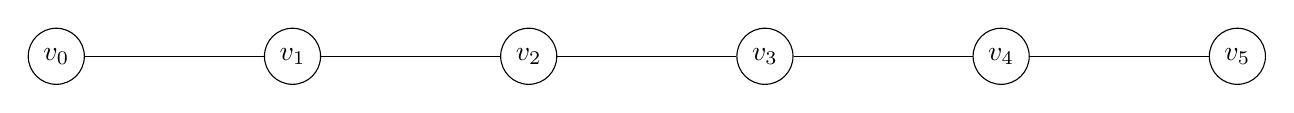
\begin{tikzpicture}[scale=1.5]
  % Define number of vertices (k+1 vertices)
  \def\k{5}  % Path of length k=5
  
  % Place vertices on a horizontal line
  \foreach \i in {0,...,\k} {
    \node[draw, circle, fill=white, minimum size=0.6cm] (v\i) at (\i*2,0) {$v_{\i}$};
  }
  
  % Connect edges
  \foreach \i in {0,...,\number\numexpr\k-1} {
    \pgfmathtruncatemacro{\j}{\i+1}
    \draw (v\i) -- (v\j);
  }
\end{tikzpicture}
\caption{A path graph $P_5$ with 6 vertices.}
\end{figure}

\subsection{Degrees and Neighborhoods}

\begin{definition}
If $G$ is a graph and $v \in V(G)$, then:
\begin{itemize}
\item The neighborhood of $v$ is $N_G(v) = \{w \in V(G) : \{v,w\} \in E(G)\}$
\item The degree of $v$ is $d(v) = d_G(v) = |N_G(v)|$
\end{itemize}
\end{definition}



\begin{figure}[H]
\centering
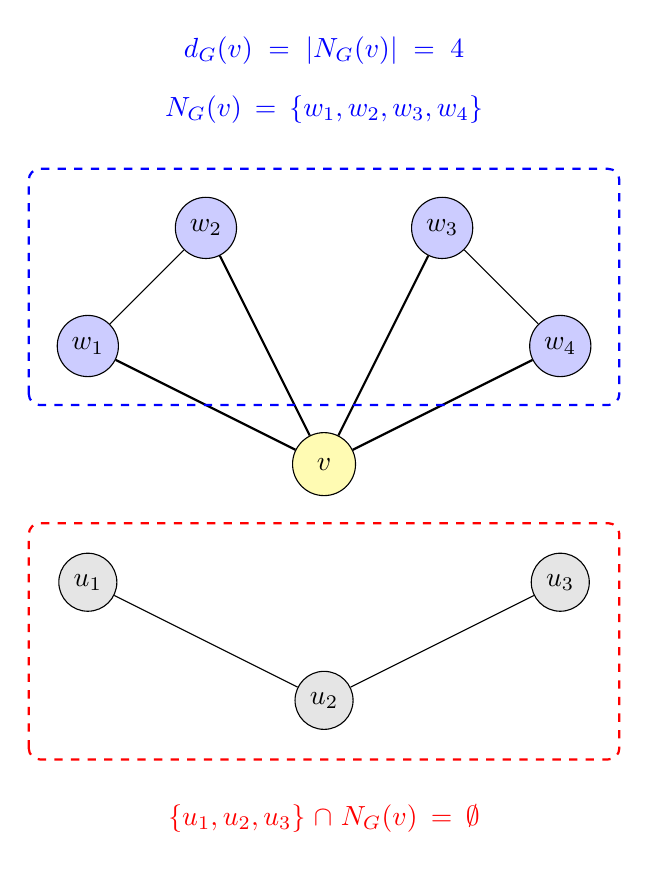
\begin{tikzpicture}[scale=1.5]
  % Central node v
  \node[draw, circle, fill=yellow!30, minimum size=0.8cm] (v) at (0,0) {$v$};
  
  % Neighbors of v
  \node[draw, circle, fill=blue!20, minimum size=0.6cm] (w1) at (-2,1) {$w_1$};
  \node[draw, circle, fill=blue!20, minimum size=0.6cm] (w2) at (-1,2) {$w_2$};
  \node[draw, circle, fill=blue!20, minimum size=0.6cm] (w3) at (1,2) {$w_3$};
  \node[draw, circle, fill=blue!20, minimum size=0.6cm] (w4) at (2,1) {$w_4$};
  
  % Non-neighbor vertices
  \node[draw, circle, fill=gray!20, minimum size=0.6cm] (u1) at (-2,-1) {$u_1$};
  \node[draw, circle, fill=gray!20, minimum size=0.6cm] (u2) at (0,-2) {$u_2$};
  \node[draw, circle, fill=gray!20, minimum size=0.6cm] (u3) at (2,-1) {$u_3$};
  
  % Edges between v and its neighbors
  \draw[thick] (v) -- (w1);
  \draw[thick] (v) -- (w2);
  \draw[thick] (v) -- (w3);
  \draw[thick] (v) -- (w4);
  
  % Other edges
  \draw (w1) -- (w2);
  \draw (w3) -- (w4);
  \draw (u1) -- (u2);
  \draw (u2) -- (u3);
  
  % Neighborhood set indicator
  \draw[blue, thick, dashed, rounded corners] (-2.5,0.5) rectangle (2.5,2.5) {};
  \node[blue, text width=5cm, align=center] at (0,3) {$N_G(v) = \{w_1, w_2, w_3, w_4\}$};
  
  % Degree display - moved and color changed
  \node[blue, text width=5cm, align=center] at (0,3.5) {$d_G(v) = |N_G(v)| = 4$};
  
  % Non-neighbor set indicator
  \draw[red, thick, dashed, rounded corners] (-2.5,-2.5) rectangle (2.5,-0.5) {};
  \node[red, text width=5cm, align=center] at (0,-3) {$\{u_1, u_2, u_3\} \cap N_G(v) = \emptyset$};
\end{tikzpicture}
\caption{Example of neighborhood and degree of a vertex in a graph.}
\end{figure}

\begin{definition}[Incidence]
In graph theory, incidence refers to the relationship between vertices and edges:
\begin{itemize}[label=$\bullet$]
    \item A vertex $v$ and an edge $e$ are \textit{incident} with each other if $v$ is an endpoint of $e$.
    \item If $e = \{u, v\}$, then:
    \begin{itemize}[label=$\circ$]
        \item Edge $e$ is incident with vertices $u$ and $v$
        \item Vertex $u$ is incident with edge $e$
        \item Vertex $v$ is incident with edge $e$
    \end{itemize}
    \item The incidence relation forms the fundamental connection between vertices and edges in a graph.
\end{itemize}
\end{definition}

\subsection{Examples of Graphs and Their Vertex Degrees}

\subsubsection{Complete Graph $K_n$}
In a complete graph with $n$ vertices, every vertex is connected to all other vertices.
\begin{itemize}
    \item For any vertex $v$ in $K_n$: $\deg(v) = n-1$
    \item Example: In $K_5$, every vertex has $\deg(v) = 4$
    \item Total edges: $|E| = \frac{n(n-1)}{2} = \frac{5 \cdot 4}{2} = 10$
\end{itemize}

\begin{figure}[H]
\centering
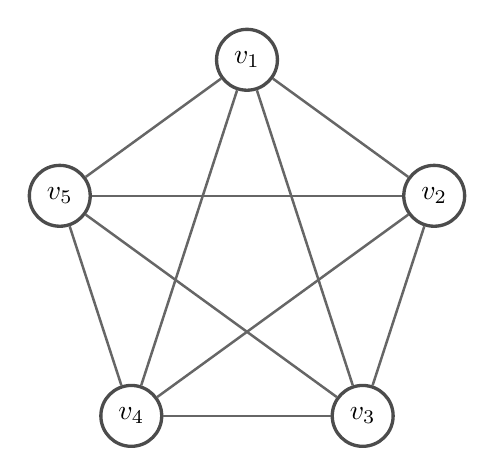
\begin{tikzpicture}
  % Define overall style for the graph
  \tikzset{
    vertex/.style={
      draw,
      circle,
      fill=white,
      minimum size=22pt,
      inner sep=0pt,
      line width=1.2pt,
      draw=black!70
    },
    edge/.style={
      draw=black!60,
      line width=0.9pt
    },
    vlabel/.style={
      font=\sffamily\bfseries,
      text=black!80
    }
  }
  
  % Create vertices at regular pentagon positions
  \def\radius{2.5cm}
  \node[vertex] (v1) at (90:\radius) {$v_1$};
  \node[vertex] (v2) at (18:\radius) {$v_2$};
  \node[vertex] (v3) at (306:\radius) {$v_3$};
  \node[vertex] (v4) at (234:\radius) {$v_4$};
  \node[vertex] (v5) at (162:\radius) {$v_5$};
  
  % Draw all edges
  \foreach \i in {1,...,5} {
    \foreach \j in {\i,...,5} {
      \ifnum\i=\j\else
        \draw[edge] (v\i) -- (v\j);
      \fi
    }
  }
\end{tikzpicture}
\caption{In this complete graph $K_5$ with 5 vertices, each vertex $v_i$ has degree 4. Every vertex is connected to all other vertices in the graph. Total number of edges = $\frac{n(n-1)}{2} = \frac{5 \cdot 4}{2} = 10$}
\end{figure}

\subsubsection{Cycle Graph $C_n$}
A cycle graph with $n$ vertices forms a closed loop.
\begin{itemize}
    \item For any vertex $v$ in $C_n$: $\deg(v) = 2$
    \item Example: In a hexagon $C_6$, every vertex has $\deg(v) = 2$
    \item Total edges: $|E| = n = 6$
\end{itemize}

\begin{center}
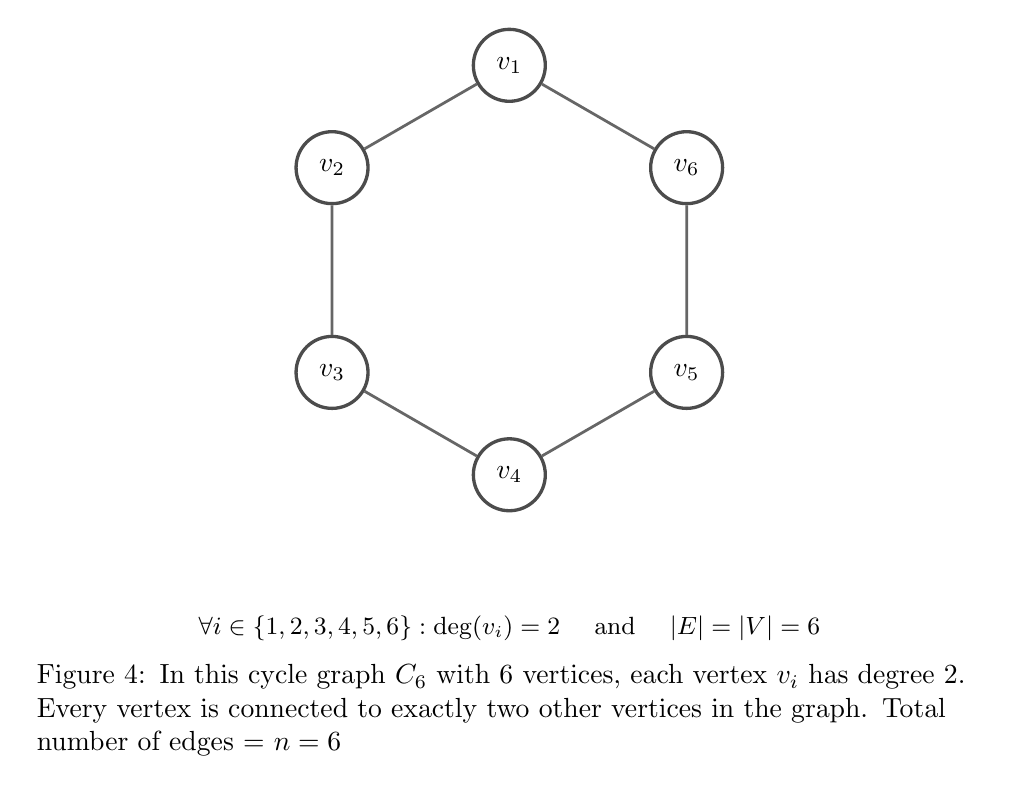
\begin{tikzpicture}[scale=1.3] % Increased scale factor for a larger graph
  % Define styles for vertices
  \tikzset{
    vertex/.style={
      draw,
      circle,
      fill=white,
      minimum size=26pt, % Increased vertex size
      inner sep=0pt,
      line width=1.2pt,
      draw=black!70
    },
    edge/.style={
      draw=black!60,
      line width=1pt % Slightly thicker edges
    }
  }
  
  % Create vertices at regular hexagon positions
  \def\n{6}
  \def\radius{2cm} % Increased radius for larger graph
  
  \foreach \i in {1,...,\n} {
    \node[vertex] (v\i) at ({360/\n*(\i-1)+90}:\radius) {$v_{\i}$};
  }
  
  % Connect vertices to form cycle
  \foreach \i in {1,...,\n} {
    \pgfmathtruncatemacro{\j}{mod(\i, \n) + 1}
    \draw[edge] (v\i) -- (v\j);
  }
  
  % Add compact formula below the graph
  \node[align=center, font=\small] at (0,-3.5) {$\forall i \in \{1,2,3,4,5,6\}: \deg(v_i) = 2 \quad$ and $\quad |E| = |V| = 6$};
  
  % Add Figure 4 caption
  \node[align=left, text width=12cm] at (0,-4.3) {
    Figure 4: In this cycle graph $C_6$ with 6 vertices, each vertex $v_i$ has degree 2. Every vertex is connected to exactly two other vertices in the graph. Total number of edges = $n = 6$
  };
\end{tikzpicture}
\end{center}
\subsubsection{Path Graph $P_n$}
A path graph with $n$ vertices forms a single path.
\begin{itemize}
    \item For endpoints: $\deg(v) = 1$
    \item For internal vertices: $\deg(v) = 2$
    \item Example: In $P_7$, the degree sequence is $(1, 2, 2, 2, 2, 2, 1)$
    \item Total edges: $|E| = n-1 = 6$
\end{itemize}

\begin{center}
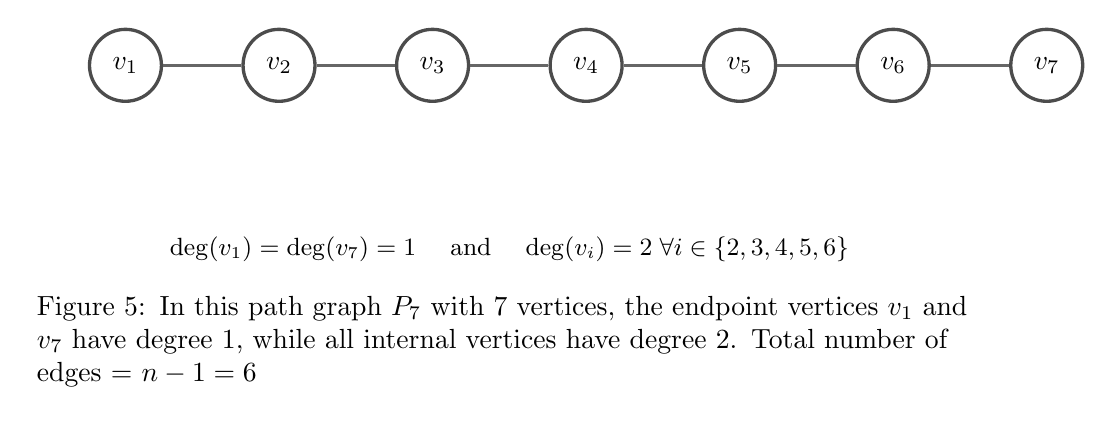
\begin{tikzpicture}[scale=1.3]
  % Define styles for vertices
  \tikzset{
    vertex/.style={
      draw,
      circle,
      fill=white,
      minimum size=26pt,
      inner sep=0pt,
      line width=1.2pt,
      draw=black!70
    },
    edge/.style={
      draw=black!60,
      line width=1pt
    }
  }
  
  % Create vertices in a horizontal line
  \def\n{7}
  \foreach \i in {1,...,\n} {
    \node[vertex] (v\i) at (\i*1.5-1.5*\n/2,0) {$v_{\i}$};
  }
  
  % Connect vertices to form path
  \foreach \i in {1,...,\number\numexpr\n-1} {
    \pgfmathtruncatemacro{\j}{\i+1}
    \draw[edge] (v\i) -- (v\j);
  }
  
  % Add compact formula below the graph
  \node[align=center, font=\small] at (0,-1.8) {$\deg(v_1) = \deg(v_7) = 1 \quad$ and $\quad \deg(v_i) = 2 \; \forall i \in \{2,3,4,5,6\}$};
  
  % Add Figure 5 caption
  \node[align=left, text width=12cm] at (0,-2.7) {
    Figure 5: In this path graph $P_7$ with 7 vertices, the endpoint vertices $v_1$ and $v_7$ have degree 1, while all internal vertices have degree 2. Total number of edges = $n-1 = 6$
  };
\end{tikzpicture}
\end{center}

\subsubsection{Star Graph $S_n$}
A star graph has one central vertex connected to $n-1$ leaf vertices.
\begin{itemize}
    \item For central vertex $c$: $\deg(c) = n-1$
    \item For any leaf vertex $v$: $\deg(v) = 1$
    \item Example: In $S_6$, the central vertex has $\deg(c) = 5$, and the 5 leaf vertices each have $\deg(v) = 1$
    \item Total edges: $|E| = n-1 = 5$
\end{itemize}

\begin{center}
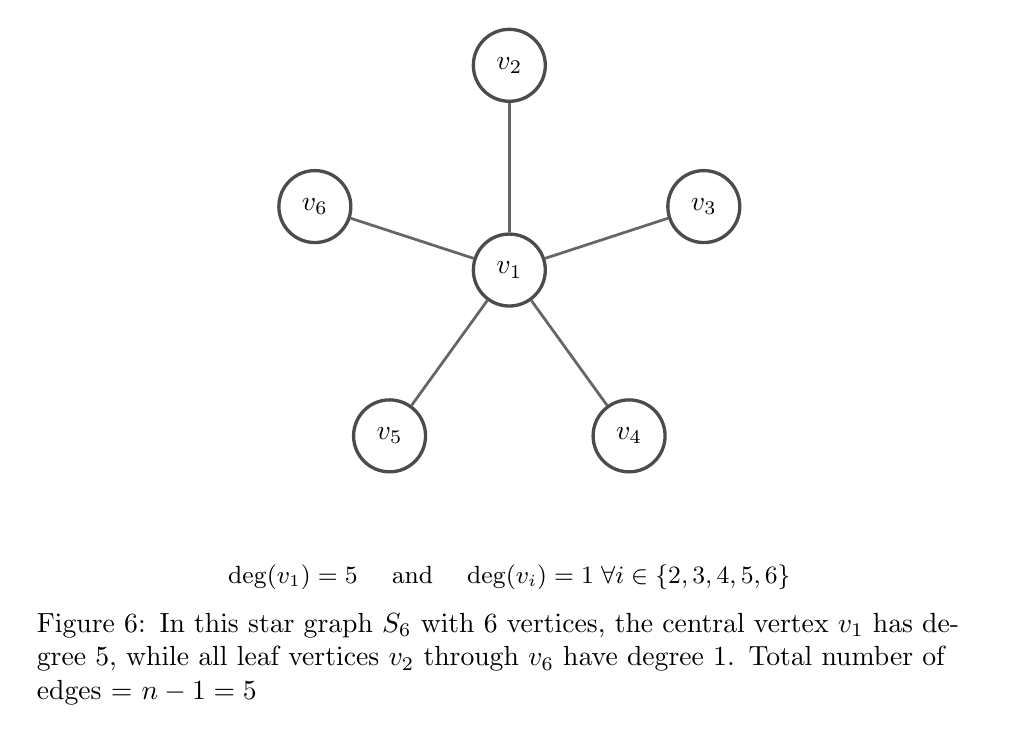
\begin{tikzpicture}[scale=1.3]
  % Define styles for vertices
  \tikzset{
    vertex/.style={
      draw,
      circle,
      fill=white,
      minimum size=26pt,
      inner sep=0pt,
      line width=1.2pt,
      draw=black!70
    },
    edge/.style={
      draw=black!60,
      line width=1pt
    }
  }
  
  % Create vertices - central and leaf vertices
  \node[vertex] (v1) at (0,0) {$v_1$};
  \node[vertex] (v2) at (0,2) {$v_2$};
  \node[vertex] (v3) at (1.9,0.62) {$v_3$};
  \node[vertex] (v4) at (1.17,-1.62) {$v_4$};
  \node[vertex] (v5) at (-1.17,-1.62) {$v_5$};
  \node[vertex] (v6) at (-1.9,0.62) {$v_6$};
  
  % Connect edges
  \draw[edge] (v1) -- (v2);
  \draw[edge] (v1) -- (v3);
  \draw[edge] (v1) -- (v4);
  \draw[edge] (v1) -- (v5);
  \draw[edge] (v1) -- (v6);
  
  % Add compact formula below the graph
  \node[align=center, font=\small] at (0,-3) {$\deg(v_1) = 5 \quad$ and $\quad \deg(v_i) = 1 \; \forall i \in \{2,3,4,5,6\}$};
  
  % Add Figure 6 caption
  \node[align=left, text width=12cm] at (0,-3.8) {
    Figure 6: In this star graph $S_6$ with 6 vertices, the central vertex $v_1$ has degree 5, while all leaf vertices $v_2$ through $v_6$ have degree 1. Total number of edges = $n-1 = 5$
  };
\end{tikzpicture}
\end{center}

\subsubsection{Wheel Graph $W_n$}
A wheel graph is formed by connecting a single vertex to all vertices of a cycle.
\begin{itemize}
    \item For central vertex $c$: $\deg(c) = n-1$
    \item For vertices on the cycle: $\deg(v) = 3$
    \item Example: In $W_8$, the central vertex has $\deg(c) = 7$, and the 7 outer vertices each have $\deg(v) = 3$
    \item Total edges: $|E| = 2(n-1) = 14$
\end{itemize}

\begin{center}
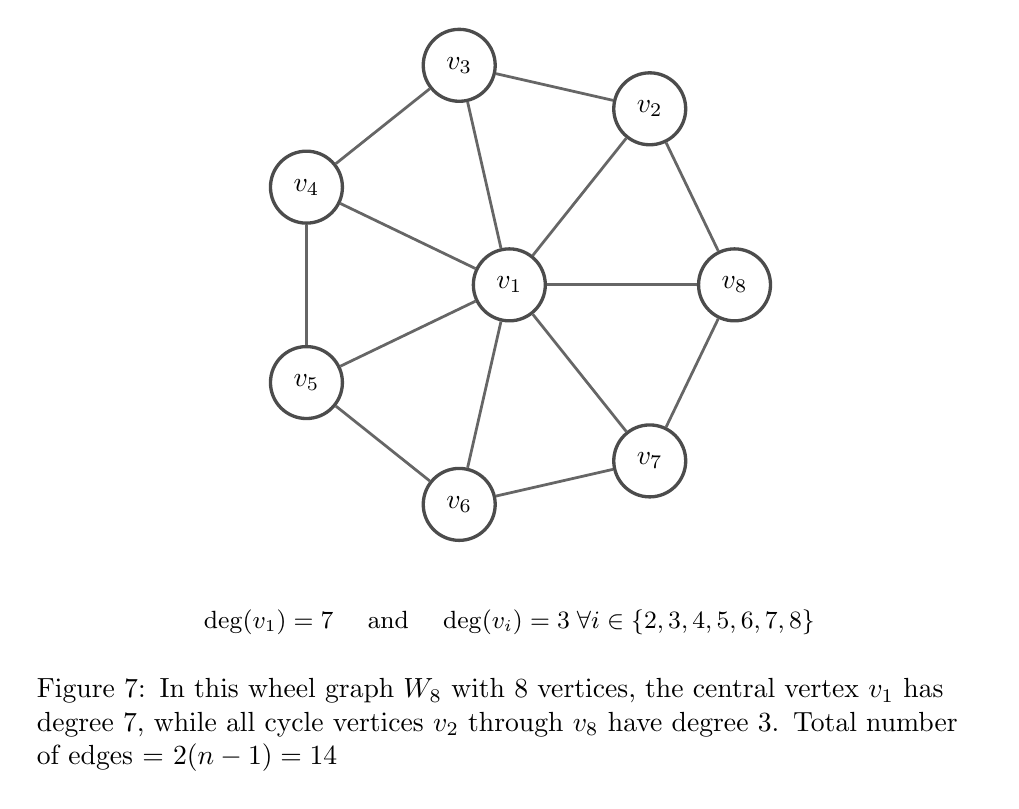
\begin{tikzpicture}[scale=1.3]
  % Define styles for vertices
  \tikzset{
    vertex/.style={
      draw,
      circle,
      fill=white,
      minimum size=26pt,
      inner sep=0pt,
      line width=1.2pt,
      draw=black!70
    },
    edge/.style={
      draw=black!60,
      line width=1pt
    }
  }
  
  % Create central vertex
  \node[vertex] (v1) at (0,0) {$v_1$};
  
  % Create outer cycle vertices
  \def\n{7}
  \def\radius{2.2cm}
  
  \foreach \i in {2,...,\number\numexpr\n+1} {
    \pgfmathtruncatemacro{\j}{\i-1}
    \node[vertex] (v\i) at ({360/\n*\j}:\radius) {$v_{\i}$};
  }
  
  % Draw cycle edges
  \foreach \i in {2,...,\number\numexpr\n+1} {
    \pgfmathtruncatemacro{\j}{mod(\i-1, \n) + 2}
    \draw[edge] (v\i) -- (v\j);
  }
  
  % Draw spokes from center to cycle
  \foreach \i in {2,...,\number\numexpr\n+1} {
    \draw[edge] (v1) -- (v\i);
  }
  
  % Add compact formula below the graph
  \node[align=center, font=\small] at (0,-3.3) {$\deg(v_1) = 7 \quad$ and $\quad \deg(v_i) = 3 \; \forall i \in \{2,3,4,5,6,7,8\}$};
  
  % Add Figure 7 caption
  \node[align=left, text width=12cm] at (0,-4.3) {
    Figure 7: In this wheel graph $W_8$ with 8 vertices, the central vertex $v_1$ has degree 7, while all cycle vertices $v_2$ through $v_8$ have degree 3. Total number of edges = $2(n-1) = 14$
  };
\end{tikzpicture}
\end{center}

\subsubsection{Complete Bipartite Graph $K_{m,n}$}
A complete bipartite graph has two sets of vertices (with $m$ and $n$ vertices) where every vertex in the first set is connected to every vertex in the second set.
\begin{itemize}
    \item For vertices in the first set: $\deg(v) = n$
    \item For vertices in the second set: $\deg(v) = m$
    \item Example: In $K_{3,4}$, the 3 vertices in the first set each have $\deg(v) = 4$, and the 4 vertices in the second set each have $\deg(v) = 3$
    \item Total edges: $|E| = m \cdot n = 12$
\end{itemize}

\begin{center}
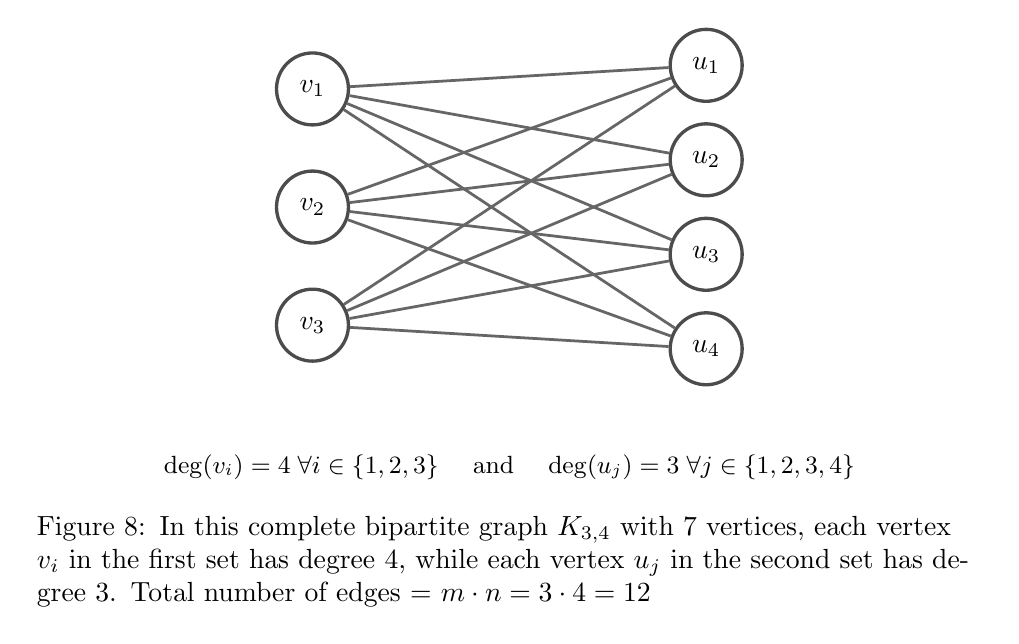
\begin{tikzpicture}[scale=1.0]
  % Define styles for vertices
  \tikzset{
    vertex/.style={
      draw,
      circle,
      fill=white,
      minimum size=26pt,
      inner sep=0pt,
      line width=1.2pt,
      draw=black!70
    },
    edge/.style={
      draw=black!60,
      line width=1pt
    }
  }
  
  % Left set (m=3)
  \node[vertex] (v1) at (-2.5,1.5) {$v_1$};
  \node[vertex] (v2) at (-2.5,0) {$v_2$};
  \node[vertex] (v3) at (-2.5,-1.5) {$v_3$};
  
  % Right set (n=4)
  \node[vertex] (u1) at (2.5,1.8) {$u_1$};
  \node[vertex] (u2) at (2.5,0.6) {$u_2$};
  \node[vertex] (u3) at (2.5,-0.6) {$u_3$};
  \node[vertex] (u4) at (2.5,-1.8) {$u_4$};
  
  % Connect each vertex in left set to each vertex in right set
  \foreach \i in {1,2,3} {
    \foreach \j in {1,2,3,4} {
      \draw[edge] (v\i) -- (u\j);
    }
  }
  
  % Add compact formula below the graph
  \node[align=center, font=\small] at (0,-3.3) {$\deg(v_i) = 4 \; \forall i \in \{1,2,3\} \quad$ and $\quad \deg(u_j) = 3 \; \forall j \in \{1,2,3,4\}$};
  
  % Add Figure 8 caption
  \node[align=left, text width=12cm] at (0,-4.5) {
    Figure 8: In this complete bipartite graph $K_{3,4}$ with 7 vertices, each vertex $v_i$ in the first set has degree 4, while each vertex $u_j$ in the second set has degree 3. Total number of edges = $m \cdot n = 3 \cdot 4 = 12$
  };
\end{tikzpicture}
\end{center}

\subsubsection{Regular Graph}
In a $k$-regular graph, every vertex has the same degree $k$.
\begin{itemize}
    \item For any vertex $v$: $\deg(v) = k$
    \item Example: In a 3-regular graph (cubic graph), every vertex has $\deg(v) = 3$
    \item Total edges in a $k$-regular graph with $n$ vertices: $|E| = \frac{kn}{2}$
\end{itemize}

\begin{center}
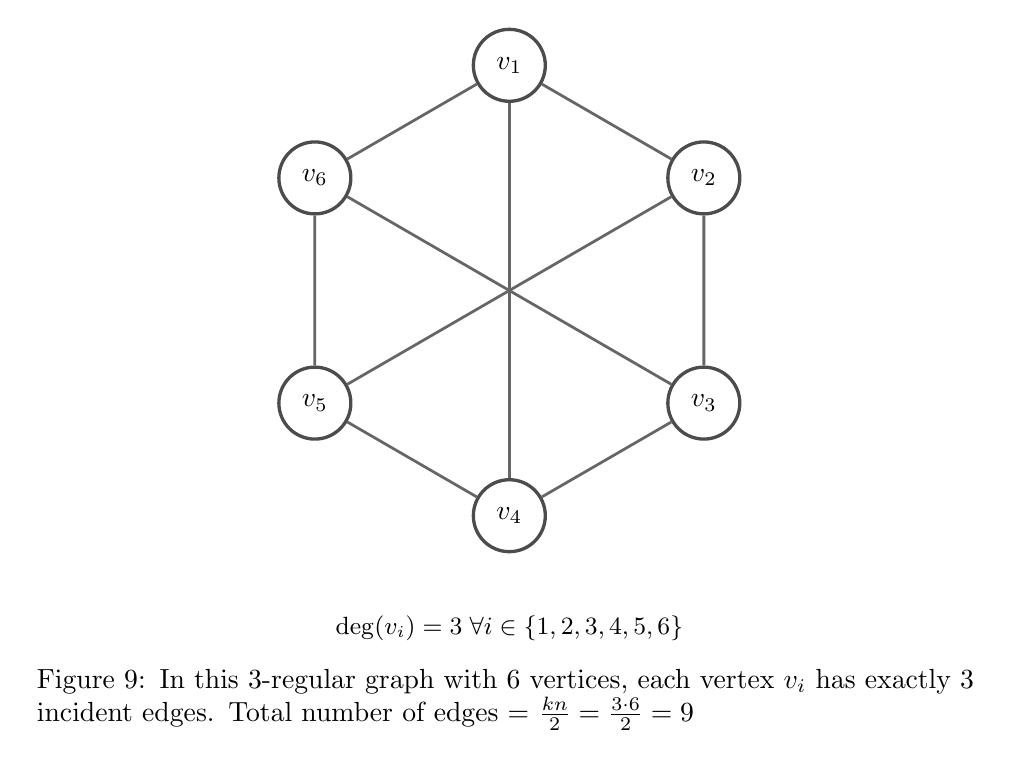
\begin{tikzpicture}[scale=1.3]
  \tikzset{
    vertex/.style={
      draw,
      circle,
      fill=white,
      minimum size=26pt,
      inner sep=0pt,
      line width=1.2pt,
      draw=black!70
    },
    edge/.style={
      draw=black!60,
      line width=1pt
    }
  }
  
  \node[vertex] (v1) at (0,2.2) {$v_1$};
  \node[vertex] (v2) at (1.9,1.1) {$v_2$};
  \node[vertex] (v3) at (1.9,-1.1) {$v_3$};
  \node[vertex] (v4) at (0,-2.2) {$v_4$};
  \node[vertex] (v5) at (-1.9,-1.1) {$v_5$};
  \node[vertex] (v6) at (-1.9,1.1) {$v_6$};
  
  \draw[edge] (v1) -- (v2) -- (v3) -- (v4) -- (v5) -- (v6) -- (v1);
  \draw[edge] (v1) -- (v4);
  \draw[edge] (v2) -- (v5);
  \draw[edge] (v3) -- (v6);
  
  \node[align=center, font=\small] at (0,-3.3) {$\deg(v_i) = 3 \; \forall i \in \{1,2,3,4,5,6\}$};
  
  \node[align=left, text width=12cm] at (0,-4.0) {
    Figure 9: In this 3-regular graph with 6 vertices, each vertex $v_i$ has exactly 3 incident edges. Total number of edges = $\frac{kn}{2} = \frac{3 \cdot 6}{2} = 9$
  };
\end{tikzpicture}
\end{center}


\subsubsection{Hypercube Graph $Q_n$}
In an $n$-dimensional hypercube, every vertex has degree $n$.
\begin{itemize}
    \item For any vertex $v$ in $Q_n$: $\deg(v) = n$
    \item Example: In $Q_3$ (3-dimensional cube), every vertex has $\deg(v) = 3$
    \item Total vertices: $|V| = 2^n$
    \item Total edges: $|E| = n \cdot 2^{n-1}$
\end{itemize}

\begin{center}
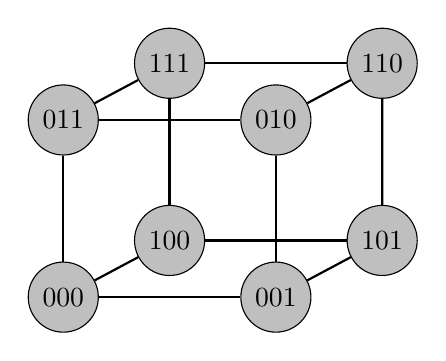
\begin{tikzpicture}[scale=0.9]
  % Q_3 (3-dimensional hypercube)
  % Front square
  \node[draw, circle, fill=lightgray, minimum size=0.7cm] (v000) at (0,0) {$000$};
  \node[draw, circle, fill=lightgray, minimum size=0.7cm] (v001) at (3,0) {$001$};
  \node[draw, circle, fill=lightgray, minimum size=0.7cm] (v010) at (3,2.5) {$010$};
  \node[draw, circle, fill=lightgray, minimum size=0.7cm] (v011) at (0,2.5) {$011$};
  
  % Back square
  \node[draw, circle, fill=lightgray, minimum size=0.7cm] (v100) at (1.5,0.8) {$100$};
  \node[draw, circle, fill=lightgray, minimum size=0.7cm] (v101) at (4.5,0.8) {$101$};
  \node[draw, circle, fill=lightgray, minimum size=0.7cm] (v110) at (4.5,3.3) {$110$};
  \node[draw, circle, fill=lightgray, minimum size=0.7cm] (v111) at (1.5,3.3) {$111$};
  
  % Front face edges
  \draw[thick] (v000) -- (v001);
  \draw[thick] (v001) -- (v010);
  \draw[thick] (v010) -- (v011);
  \draw[thick] (v011) -- (v000);
  
  % Back face edges
  \draw[thick] (v100) -- (v101);
  \draw[thick] (v101) -- (v110);
  \draw[thick] (v110) -- (v111);
  \draw[thick] (v111) -- (v100);
  
  % Connections between front and back faces
  \draw[thick] (v000) -- (v100);
  \draw[thick] (v001) -- (v101);
  \draw[thick] (v010) -- (v110);
  \draw[thick] (v011) -- (v111);
\end{tikzpicture}
\end{center}

\begin{center}
    \vspace{0.5cm}
{\centering
\small $\deg(v) = 3 \; \forall v \in V(Q_3)$
\par}

\vspace{0.5cm}
{\centering
\footnotesize Figure 10: Hypercube graph $Q_3$ with vertices labeled by binary strings. Each vertex has degree 3, with connections to neighbors that differ in exactly one bit position.
\par}
\end{center}

\subsubsection{Petersen Graph}
The Petersen graph is a specific 3-regular graph with 10 vertices.
\begin{itemize}
    \item For any vertex $v$: $\deg(v) = 3$
    \item Total edges: $|E| = 15$
\end{itemize}

\begin{center}
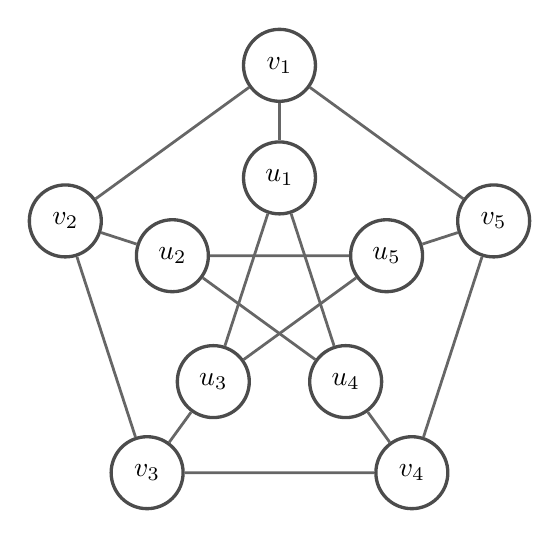
\begin{tikzpicture}[scale=1.3]
  \tikzset{
    vertex/.style={
      draw,
      circle,
      fill=white,
      minimum size=26pt,
      inner sep=0pt,
      line width=1.2pt,
      draw=black!70
    },
    edge/.style={
      draw=black!60,
      line width=1pt
    }
  }
  
  % Outer vertices
  \foreach \i in {1,...,5} {
    \node[vertex] (v\i) at ({90+72*(\i-1)}:2.2) {$v_{\i}$};
  }
  
  % Inner vertices
  \foreach \i in {1,...,5} {
    \node[vertex] (u\i) at ({90+72*(\i-1)}:1.1) {$u_{\i}$};
  }
  
  % Outer edges
  \foreach \i in {1,...,5} {
    \pgfmathtruncatemacro{\j}{mod(\i,5)+1}
    \draw[edge] (v\i) -- (v\j);
  }
  
  % Spoke edges
  \foreach \i in {1,...,5} {
    \draw[edge] (v\i) -- (u\i);
  }
  
  % Inner star edges
  \foreach \i in {1,...,5} {
    \pgfmathtruncatemacro{\j}{mod(\i+1,5)+1}
    \draw[edge] (u\i) -- (u\j);
  }
\end{tikzpicture}
\end{center}

% Formula and caption
\vspace{0.5cm}
{\centering
\small $\deg(v_i) = \deg(u_i) = 3 \; \forall i \in \{1,2,3,4,5\}$
\par}

\vspace{0.5cm}
{\centering
\footnotesize Figure 11: Petersen graph with 10 vertices. Each vertex has degree 3, with a total of 15 edges. This is a famous non-Hamiltonian 3-regular graph.
\par}

\subsection{Mathematical Properties Related to Degrees}

\subsubsection{Handshaking Lemma}
The sum of all degrees equals twice the number of edges:
\begin{equation}
\sum_{v \in V} \deg(v) = 2|E|
\end{equation}

\begin{center}
\begin{tikzpicture}[scale=1.5]
  \tikzset{
    vertex/.style={
      draw,
      circle,
      fill=white,
      minimum size=26pt,
      inner sep=0pt,
      line width=1.2pt,
      draw=black!70
    },
    edge/.style={
      draw=black!60,
      line width=1pt
    },
    elabel/.style={
      midway,
      font=\small
    }
  }
\end{tikzpicture}
\end{center}
  
\begin{center}
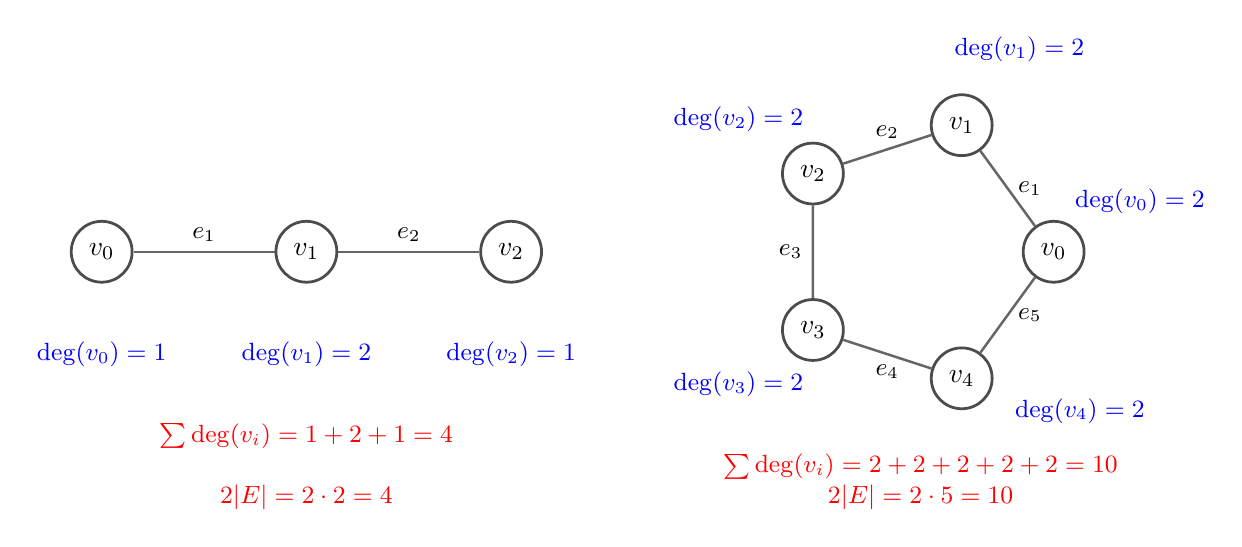
\begin{tikzpicture}[scale=1.3]
  \tikzset{
    vertex/.style={
      draw,
      circle,
      fill=white,
      minimum size=22pt,
      inner sep=0pt,
      line width=1pt,
      draw=black!70
    },
    edge/.style={
      draw=black!60,
      line width=0.9pt
    },
    elabel/.style={
      midway,
      font=\small
    }
  }
  
  % First example: Path graph
  \begin{scope}[shift={(-4,0)}]
    % Vertices
    \node[vertex] (v0) at (0,0) {$v_0$};
    \node[vertex] (v1) at (2,0) {$v_1$};
    \node[vertex] (v2) at (4,0) {$v_2$};
    
    % Edges
    \draw[edge] (v0) -- (v1) node[elabel, above] {$e_1$};
    \draw[edge] (v1) -- (v2) node[elabel, above] {$e_2$};
    
    % Degree display
    \node[font=\small, text=blue] at (0,-1) {$\deg(v_0) = 1$};
    \node[font=\small, text=blue] at (2,-1) {$\deg(v_1) = 2$};
    \node[font=\small, text=blue] at (4,-1) {$\deg(v_2) = 1$};
    
    % Sum calculation
    \node[font=\small, text=red] at (2,-1.8) {$\sum \deg(v_i) = 1 + 2 + 1 = 4$};
    \node[font=\small, text=red] at (2,-2.4) {$2|E| = 2 \cdot 2 = 4$};
  \end{scope}
  
  % Second example: Cycle graph
  \begin{scope}[shift={(4,0)}]
    % Vertices
    \node[vertex] (v0) at (0:1.3cm) {$v_0$};
    \node[vertex] (v1) at (72:1.3cm) {$v_1$};
    \node[vertex] (v2) at (144:1.3cm) {$v_2$};
    \node[vertex] (v3) at (216:1.3cm) {$v_3$};
    \node[vertex] (v4) at (288:1.3cm) {$v_4$};
    
    % Edges
    \draw[edge] (v0) -- (v1) node[elabel, right] {$e_1$};
    \draw[edge] (v1) -- (v2) node[elabel, above] {$e_2$};
    \draw[edge] (v2) -- (v3) node[elabel, left] {$e_3$};
    \draw[edge] (v3) -- (v4) node[elabel, below] {$e_4$};
    \draw[edge] (v4) -- (v0) node[elabel, right] {$e_5$};
    
    % Degree display
    \node[font=\small, text=blue] at (13:2.2cm) {$\deg(v_0) = 2$};
    \node[font=\small, text=blue] at (64:2.2cm) {$\deg(v_1) = 2$};
    \node[font=\small, text=blue] at (144:2.2cm) {$\deg(v_2) = 2$};
    \node[font=\small, text=blue] at (216:2.2cm) {$\deg(v_3) = 2$};
    \node[font=\small, text=blue] at (315:2.2cm) {$\deg(v_4) = 2$};
    
    % Sum calculation
    \node[font=\small, text=red] at (0,-2.1) {$\sum \deg(v_i) = 2 + 2 + 2 + 2 + 2 = 10$};
    \node[font=\small, text=red] at (0,-2.4) {$2|E| = 2 \cdot 5 = 10$};
  \end{scope}
\end{tikzpicture}
\end{center}

% Caption
\vspace{0.3cm}
{\centering
\footnotesize Figure 12: Illustration of the Handshaking Lemma. Left: A path graph with 3 vertices and 2 edges. Right: A cycle graph with 5 vertices and 5 edges. In both cases, the sum of vertex degrees equals twice the number of edges.
\par}
\begin{example}
Consider a graph with vertex set $V = \{1, 2, 3, 4\}$ and edge set $E = \{\{1,2\}, \{1,3\}, \{1,4\}, \{2,3\}, \{3,4\}\}$.
\begin{align*}
\sum_{v \in V} d(v) &= d(1) + d(2) + d(3) + d(4)\\
&= 3 + 2 + 3 + 2\\
&= 10
\end{align*}
And $2|E| = 2 \cdot 5 = 10$.
\end{example}

\subsubsection{Degree Sequence}
The non-increasing sequence of vertex degrees.
\begin{itemize}
    \item Example: A graph with degree sequence $(4,3,3,2,2,1,1)$ has 7 vertices with varying connectivity
    \item Valid degree sequences must sum to an even number
\end{itemize}
\subsubsection{Average Degree}
The average degree of vertices in a graph $G = (V,E)$ is:
\begin{equation}
\text{avg}(\deg) = \frac{\sum_{v \in V} \deg(v)}{|V|} = \frac{2|E|}{|V|}
\end{equation}
\subsubsection{Maximum and Minimum Degree}
\begin{align}
\Delta(G) &= \max\{\deg(v) \mid v \in V\} \\
\delta(G) &= \min\{\deg(v) \mid v \in V\}
\end{align}
\begin{corollary}
In any graph, there are an even number of vertices of odd degree.
\end{corollary}

\begin{center}
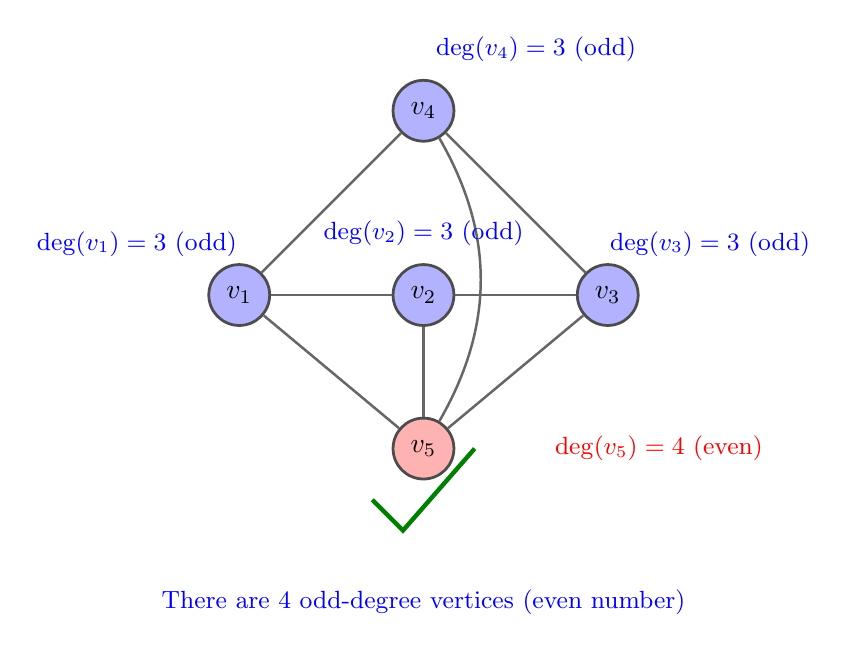
\begin{tikzpicture}[scale=1.3]
  \tikzset{
    vertex/.style={
      draw,
      circle,
      fill=white,
      minimum size=22pt,
      inner sep=0pt,
      line width=1pt,
      draw=black!70
    },
    oddvertex/.style={
      draw,
      circle,
      fill=blue!30,
      minimum size=22pt,
      inner sep=0pt,
      line width=1pt,
      draw=black!70
    },
    evenvertex/.style={
      draw,
      circle,
      fill=red!30,
      minimum size=22pt,
      inner sep=0pt,
      line width=1pt,
      draw=black!70
    },
    edge/.style={
      draw=black!60,
      line width=0.9pt
    }
  }
  
  % Nodes
  \node[oddvertex] (v1) at (-1.8,0) {$v_1$};
  \node[oddvertex] (v2) at (0,0) {$v_2$};
  \node[oddvertex] (v3) at (1.8,0) {$v_3$};
  \node[oddvertex] (v4) at (0,1.8) {$v_4$};
  \node[evenvertex] (v5) at (0,-1.5) {$v_5$};
  
  % Edges
  \draw[edge] (v1) -- (v2);
  \draw[edge] (v2) -- (v3);
  \draw[edge] (v1) -- (v4);
  \draw[edge] (v3) -- (v4);
  \draw[edge] (v1) -- (v5);
  \draw[edge] (v2) -- (v5);
  \draw[edge] (v3) -- (v5);
  \draw[edge] (v4) to[bend left=30] (v5);
  
  % Degree display
  \node[align=center, blue, font=\small] at (-2.8,0.5) {$\deg(v_1)=3$ (odd)};
  \node[align=center, blue, font=\small] at (0,0.6) {$\deg(v_2)=3$ (odd)};
  \node[align=center, blue, font=\small] at (2.8,0.5) {$\deg(v_3)=3$ (odd)};
  \node[align=center, blue, font=\small] at (1.1,2.4) {$\deg(v_4)=3$ (odd)};
  \node[align=center, red, font=\small] at (2.3,-1.5) {$\deg(v_5)=4$ (even)};
  
  % Green checkmark
  \draw[ultra thick, green!50!black] (-0.5,-2) -- (-0.2,-2.3) -- (0.5,-1.5);
  
  % Conclusion
  \node[align=center, blue, font=\small] at (0,-3) {There are 4 odd-degree vertices (even number)};
\end{tikzpicture}
\end{center}

% Caption
\vspace{0.3cm}
{\centering
\footnotesize Figure 14: A graph illustrating the handshaking lemma's corollary that any graph must contain an even number of odd-degree vertices. This example has 4 vertices with odd degree (shown in blue) and 1 vertex with even degree (shown in red).
\par}

\subsubsection{Isolated and Pendant Vertices}
\begin{itemize}
    \item Isolated vertex: $\deg(v) = 0$
    \item Pendant vertex (leaf): $\deg(v) = 1$
    \item Example: A tree with $n$ vertices has exactly $n-2$ vertices of degree $\geq 2$ and at least 2 leaves
\end{itemize}
\begin{center}
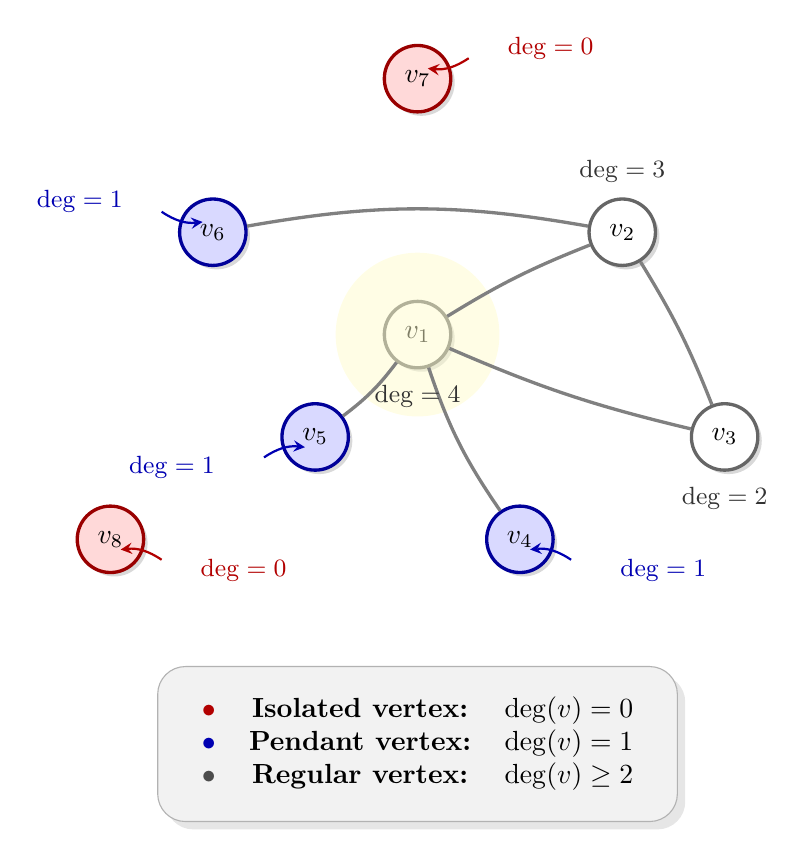
\begin{tikzpicture}[scale=1.3]
  \tikzset{
    vertex/.style={
      draw,
      circle,
      fill=white,
      minimum size=24pt,
      inner sep=0pt,
      line width=1.2pt,
      draw=black!60,
      drop shadow={shadow xshift=0.5mm, shadow yshift=-0.5mm, opacity=0.3}
    },
    isolatedvertex/.style={
      draw,
      circle,
      fill=red!15,
      minimum size=24pt,
      inner sep=0pt,
      line width=1.2pt,
      draw=red!60!black,
      drop shadow={shadow xshift=0.5mm, shadow yshift=-0.5mm, opacity=0.3}
    },
    pendantvertex/.style={
      draw,
      circle,
      fill=blue!15,
      minimum size=24pt,
      inner sep=0pt,
      line width=1.2pt,
      draw=blue!60!black,
      drop shadow={shadow xshift=0.5mm, shadow yshift=-0.5mm, opacity=0.3}
    },
    edge/.style={
      draw=black!50,
      line width=1.2pt
    },
    label/.style={
      font=\sffamily\small,
      align=center
    }
  }
  
  % Create a graph with isolated and pendant vertices
  \node[vertex] (v1) at (0,0) {$v_1$};
  \node[vertex] (v2) at (2,1) {$v_2$};
  \node[vertex] (v3) at (3,-1) {$v_3$};
  \node[pendantvertex] (v4) at (1,-2) {$v_4$};
  \node[pendantvertex] (v5) at (-1,-1) {$v_5$};
  \node[pendantvertex] (v6) at (-2,1) {$v_6$};
  \node[isolatedvertex] (v7) at (0,2.5) {$v_7$};
  \node[isolatedvertex] (v8) at (-3,-2) {$v_8$};
  
  % Add node highlights
  \path[fill=yellow!20, opacity=0.5] (v1.center) circle (0.8cm);
  
  % Connect edges with slight curves for aesthetics
  \draw[edge] (v1) to[bend left=5] (v2);
  \draw[edge] (v1) to[bend right=5] (v3);
  \draw[edge] (v2) to[bend left=5] (v3);
  \draw[edge] (v1) to[bend right=8] (v4);
  \draw[edge] (v1) to[bend left=8] (v5);
  \draw[edge] (v2) to[bend right=10] (v6);
  
  % Add degree information with elegant styling
  \node[label, text=black!80] at (0,-0.6) {$\deg=4$};
  \node[label, text=black!80] at (2,1.6) {$\deg=3$};
  \node[label, text=black!80] at (3,-1.6) {$\deg=2$};
  
  % Pendant vertices labels with elegant arrows
  \draw[->, thick, blue!70!black, >=stealth] (1.5,-2.2) to[bend right=20] (1.1,-2.1);
  \node[label, text=blue!70!black] at (2.4,-2.3) {$\deg=1$};
  
  \draw[->, thick, blue!70!black, >=stealth] (-1.5,-1.2) to[bend left=20] (-1.1,-1.1);
  \node[label, text=blue!70!black] at (-2.4,-1.3) {$\deg=1$};
  
  \draw[->, thick, blue!70!black, >=stealth] (-2.5,1.2) to[bend right=20] (-2.1,1.1);
  \node[label, text=blue!70!black] at (-3.3,1.3) {$\deg=1$};
  
  % Isolated vertices labels with elegant arrows
  \draw[->, thick, red!70!black, >=stealth] (0.5,2.7) to[bend left=20] (0.1,2.6);
  \node[label, text=red!70!black] at (1.3,2.8) {$\deg=0$};
  
  \draw[->, thick, red!70!black, >=stealth] (-2.5,-2.2) to[bend right=20] (-2.9,-2.1);
  \node[label, text=red!70!black] at (-1.7,-2.3) {$\deg=0$};
  
  % Add stylish legend
  \node[draw=black!30, rounded corners=10pt, fill=black!5, inner sep=10pt, drop shadow={shadow xshift=1mm, shadow yshift=-1mm, opacity=0.2}] at (0,-4) {
    \begin{tabular}{lcl}
      \textcolor{red!70!black}{$\bullet$} & \textbf{Isolated vertex:} & $\deg(v) = 0$ \\
      \textcolor{blue!70!black}{$\bullet$} & \textbf{Pendant vertex:} & $\deg(v) = 1$ \\
      \textcolor{black!70}{$\bullet$} & \textbf{Regular vertex:} & $\deg(v) \geq 2$ \\
    \end{tabular}
  };
\end{tikzpicture}
\end{center}

% Caption
\vspace{0.3cm}
{\centering
\footnotesize Figure 15: Illustration of special vertex types based on degree. The center vertex $v_1$ (highlighted) connects to both regular vertices and pendant vertices, while isolated vertices remain disconnected from the graph.
\par}

\subsection{Subgraphs}
\begin{definition}
A graph $F$ is a subgraph of graph $G$ if $V(F) \subseteq V(G)$ and $E(F) \subseteq E(G)$, written $F \subseteq G$.
\end{definition}

\begin{center}
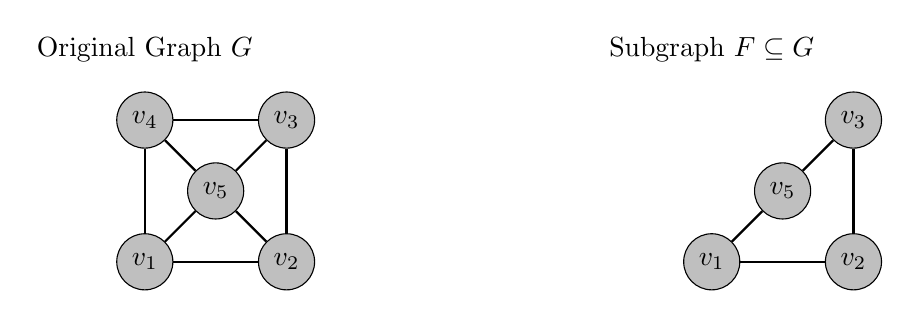
\begin{tikzpicture}[scale=0.9]
  % Original graph G
  \begin{scope}[shift={(-4,0)}]
    \node[align=center] at (0,3) {Original Graph $G$};
    
    % Vertices
    \node[draw, circle, fill=lightgray, minimum size=0.7cm] (v1) at (0,0) {$v_1$};
    \node[draw, circle, fill=lightgray, minimum size=0.7cm] (v2) at (2,0) {$v_2$};
    \node[draw, circle, fill=lightgray, minimum size=0.7cm] (v3) at (2,2) {$v_3$};
    \node[draw, circle, fill=lightgray, minimum size=0.7cm] (v4) at (0,2) {$v_4$};
    \node[draw, circle, fill=lightgray, minimum size=0.7cm] (v5) at (1,1) {$v_5$};
    
    % Edges
    \draw[thick] (v1) -- (v2);
    \draw[thick] (v2) -- (v3);
    \draw[thick] (v3) -- (v4);
    \draw[thick] (v4) -- (v1);
    \draw[thick] (v1) -- (v5);
    \draw[thick] (v2) -- (v5);
    \draw[thick] (v3) -- (v5);
    \draw[thick] (v4) -- (v5);
  \end{scope}
  
  % Subgraph F
  \begin{scope}[shift={(4,0)}]
    \node[align=center] at (0,3) {Subgraph $F \subseteq G$};
    
    % Vertices
    \node[draw, circle, fill=lightgray, minimum size=0.7cm] (u1) at (0,0) {$v_1$};
    \node[draw, circle, fill=lightgray, minimum size=0.7cm] (u2) at (2,0) {$v_2$};
    \node[draw, circle, fill=lightgray, minimum size=0.7cm] (u3) at (2,2) {$v_3$};
    \node[draw, circle, fill=lightgray, minimum size=0.7cm] (u5) at (1,1) {$v_5$};
    
    % Selected edges
    \draw[thick] (u1) -- (u2);
    \draw[thick] (u2) -- (u3);
    \draw[thick] (u1) -- (u5);
    \draw[thick] (u3) -- (u5);
  \end{scope}
\end{tikzpicture}
\end{center}

% Caption
\vspace{0.3cm}
{\centering
\footnotesize Figure 16: Illustration of a subgraph relationship. The left diagram shows the original graph $G$ with 5 vertices and 8 edges. The right diagram shows a subgraph $F \subseteq G$ where vertex $v_4$ has been removed, along with its incident edges. Additionally, some edges between the remaining vertices ($v_2$-$v_5$ and $v_3$-$v_4$) have been removed, demonstrating that a subgraph maintains subset relationships for both vertex and edge sets.
\par}

\begin{definition}
Graph $F$ is a spanning subgraph of $G$ if $V(F) = V(G)$.
\end{definition}

\begin{center}
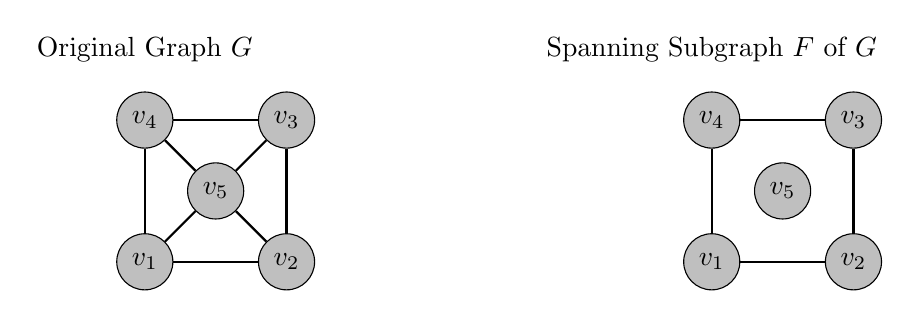
\begin{tikzpicture}[scale=0.9]
  % Original graph G
  \begin{scope}[shift={(-4,0)}]
    \node[align=center] at (0,3) {Original Graph $G$};
    
    % Vertices
    \node[draw, circle, fill=lightgray, minimum size=0.7cm] (v1) at (0,0) {$v_1$};
    \node[draw, circle, fill=lightgray, minimum size=0.7cm] (v2) at (2,0) {$v_2$};
    \node[draw, circle, fill=lightgray, minimum size=0.7cm] (v3) at (2,2) {$v_3$};
    \node[draw, circle, fill=lightgray, minimum size=0.7cm] (v4) at (0,2) {$v_4$};
    \node[draw, circle, fill=lightgray, minimum size=0.7cm] (v5) at (1,1) {$v_5$};
    
    % Edges
    \draw[thick] (v1) -- (v2);
    \draw[thick] (v2) -- (v3);
    \draw[thick] (v3) -- (v4);
    \draw[thick] (v4) -- (v1);
    \draw[thick] (v1) -- (v5);
    \draw[thick] (v2) -- (v5);
    \draw[thick] (v3) -- (v5);
    \draw[thick] (v4) -- (v5);
  \end{scope}
  
  % Spanning subgraph F
  \begin{scope}[shift={(4,0)}]
    \node[align=center] at (0,3) {Spanning Subgraph $F$ of $G$};
    
    % All vertices included (V(F) = V(G))
    \node[draw, circle, fill=lightgray, minimum size=0.7cm] (u1) at (0,0) {$v_1$};
    \node[draw, circle, fill=lightgray, minimum size=0.7cm] (u2) at (2,0) {$v_2$};
    \node[draw, circle, fill=lightgray, minimum size=0.7cm] (u3) at (2,2) {$v_3$};
    \node[draw, circle, fill=lightgray, minimum size=0.7cm] (u4) at (0,2) {$v_4$};
    \node[draw, circle, fill=lightgray, minimum size=0.7cm] (u5) at (1,1) {$v_5$};
    
    % Only some edges included (E(F) ⊆ E(G))
    \draw[thick] (u1) -- (u2);
    \draw[thick] (u2) -- (u3);
    \draw[thick] (u3) -- (u4);
    \draw[thick] (u4) -- (u1);
    % Edges connected to v5 are omitted
  \end{scope}
\end{tikzpicture}
\end{center}

% Caption
\vspace{0.3cm}
{\centering
\footnotesize Figure 17: Illustration of a spanning subgraph. The original graph $G$ (left) has 5 vertices and 8 edges, including connections from central vertex $v_5$ to all other vertices. The spanning subgraph $F$ (right) contains all vertices of $G$ but only a subset of edges, specifically removing all connections to the central vertex $v_5$. A spanning subgraph maintains the same vertex set as the original graph ($V(F) = V(G)$) but may have fewer edges ($E(F) \subseteq E(G)$).
\par}

\begin{definition}
If $X \subseteq V(G)$, the subgraph induced by $X$ is:
\begin{align*}
G[X] = (X, \{\{u,v\} \in E(G) : u, v \in X\})
\end{align*}
\end{definition}

\begin{center}
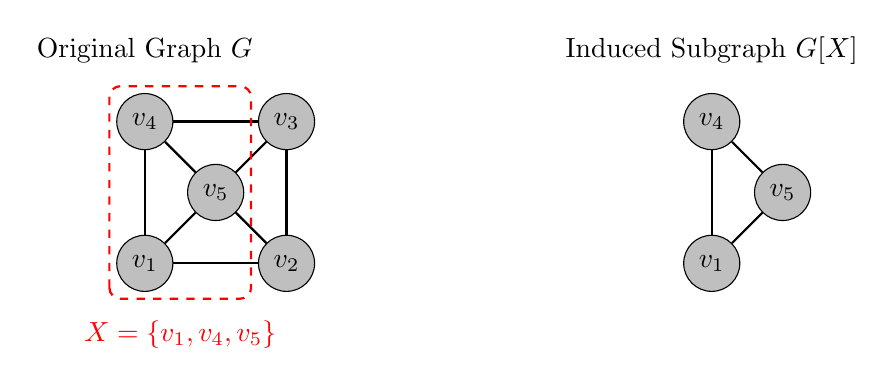
\begin{tikzpicture}[scale=0.9]
  % Original graph G
  \begin{scope}[shift={(-4,0)}]
    \node[align=center] at (0,3) {Original Graph $G$};
    
    % Vertices
    \node[draw, circle, fill=lightgray, minimum size=0.7cm] (v1) at (0,0) {$v_1$};
    \node[draw, circle, fill=lightgray, minimum size=0.7cm] (v2) at (2,0) {$v_2$};
    \node[draw, circle, fill=lightgray, minimum size=0.7cm] (v3) at (2,2) {$v_3$};
    \node[draw, circle, fill=lightgray, minimum size=0.7cm] (v4) at (0,2) {$v_4$};
    \node[draw, circle, fill=lightgray, minimum size=0.7cm] (v5) at (1,1) {$v_5$};
    
    % Edges
    \draw[thick] (v1) -- (v2);
    \draw[thick] (v2) -- (v3);
    \draw[thick] (v3) -- (v4);
    \draw[thick] (v4) -- (v1);
    \draw[thick] (v1) -- (v5);
    \draw[thick] (v2) -- (v5);
    \draw[thick] (v3) -- (v5);
    \draw[thick] (v4) -- (v5);
    
    % Highlight vertex set X for the induced subgraph
    \draw[dashed, rounded corners, red, thick] (-0.5,-0.5) rectangle (1.5,2.5);
    \node[red] at (0.5,-1) {$X = \{v_1, v_4, v_5\}$};
  \end{scope}
  
  % Induced subgraph G[X]
  \begin{scope}[shift={(4,0)}]
    \node[align=center] at (0,3) {Induced Subgraph $G[X]$};
    
    % Only vertices in X
    \node[draw, circle, fill=lightgray, minimum size=0.7cm] (u1) at (0,0) {$v_1$};
    \node[draw, circle, fill=lightgray, minimum size=0.7cm] (u4) at (0,2) {$v_4$};
    \node[draw, circle, fill=lightgray, minimum size=0.7cm] (u5) at (1,1) {$v_5$};
    
    % All original edges between vertices in X
    \draw[thick] (u1) -- (u4);
    \draw[thick] (u1) -- (u5);
    \draw[thick] (u4) -- (u5);
  \end{scope}
\end{tikzpicture}
\end{center}

% Caption
\vspace{0.3cm}
{\centering
\footnotesize Figure 18: Illustration of an induced subgraph. The original graph $G$ (left) has a subset of vertices $X = \{v_1, v_4, v_5\}$ highlighted by a red dashed rectangle. The induced subgraph $G[X]$ (right) contains exactly these vertices along with all edges from the original graph that connect vertices within this set. Unlike a general subgraph, an induced subgraph must include every edge from the original graph whose endpoints are both in the selected vertex subset.
\par}
\subsection{Walks and Paths in Graphs}
\begin{definition}
A walk in a graph is a sequence of vertices and edges:
\begin{align*}
v_0, \{v_0,v_1\}, v_1, \{v_1,v_2\}, v_2, \ldots, \{v_{k-1},v_k\}, v_k
\end{align*}
often abbreviated as $v_0, v_1, v_2, \ldots, v_k$.
The length of a walk is the number of edges in that walk.
\end{definition}
\begin{center}
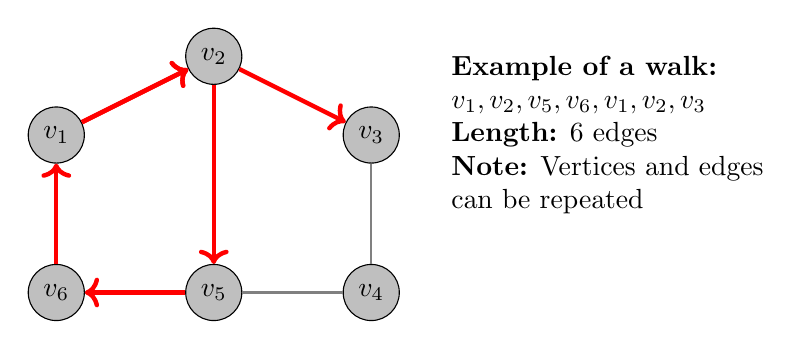
\begin{tikzpicture}[scale=1.0]
  % Basic graph
  \node[draw, circle, fill=lightgray, minimum size=0.7cm] (v1) at (0,0) {$v_1$};
  \node[draw, circle, fill=lightgray, minimum size=0.7cm] (v2) at (2,1) {$v_2$};
  \node[draw, circle, fill=lightgray, minimum size=0.7cm] (v3) at (4,0) {$v_3$};
  \node[draw, circle, fill=lightgray, minimum size=0.7cm] (v4) at (4,-2) {$v_4$};
  \node[draw, circle, fill=lightgray, minimum size=0.7cm] (v5) at (2,-2) {$v_5$};
  \node[draw, circle, fill=lightgray, minimum size=0.7cm] (v6) at (0,-2) {$v_6$};
  
  % All edges of the graph
  \draw[thick, gray] (v1) -- (v2);
  \draw[thick, gray] (v2) -- (v3);
  \draw[thick, gray] (v3) -- (v4);
  \draw[thick, gray] (v4) -- (v5);
  \draw[thick, gray] (v5) -- (v6);
  \draw[thick, gray] (v6) -- (v1);
  \draw[thick, gray] (v2) -- (v5);
  
  % Emphasize walk - can repeat vertices and edges
  \draw[->, ultra thick, red] (v1) -- (v2);
  \draw[->, ultra thick, red] (v2) -- (v5);
  \draw[->, ultra thick, red] (v5) -- (v6);
  \draw[->, ultra thick, red] (v6) -- (v1);
  \draw[->, ultra thick, red] (v1) -- (v2);
  \draw[->, ultra thick, red] (v2) -- (v3);
  
  % Walk description
  \node[align=left] at (7,0) {
    \textbf{Example of a walk:}\\
    $v_1, v_2, v_5, v_6, v_1, v_2, v_3$\\
    \textbf{Length:} 6 edges\\
    \textbf{Note:} Vertices and edges\\can be repeated
  };
\end{tikzpicture}
\end{center}

% Caption
\vspace{0.3cm}
{\centering
\footnotesize Figure 19: Illustration of a walk in graph theory. A walk is a sequence of vertices and edges where each consecutive pair of vertices in the sequence is connected by an edge. This example shows a walk of length 6 (red arrows) from $v_1$ to $v_3$ that passes through the sequence $v_1, v_2, v_5, v_6, v_1, v_2, v_3$. Unlike paths or trails, walks can repeat both vertices and edges. This walk repeats vertex $v_1$ and $v_2$, and also repeats the edge between them.
\par}
\begin{definition}
A path of length $k$ is a walk:
\begin{align*}
v_0, v_1, v_2, \ldots, v_k
\end{align*}
where all vertices are distinct.
\end{definition}
\begin{center}
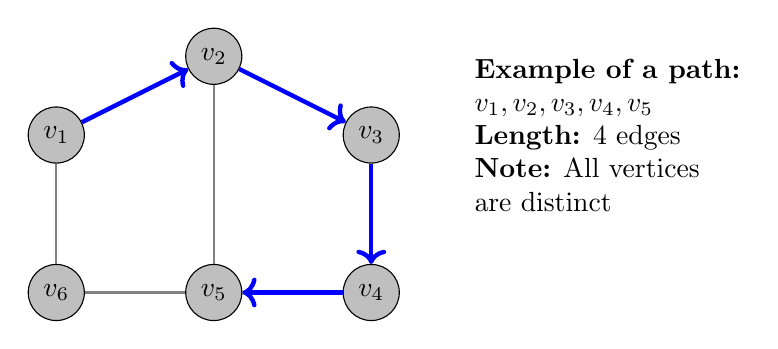
\begin{tikzpicture}[scale=1.0]
  % Basic graph
  \node[draw, circle, fill=lightgray, minimum size=0.7cm] (v1) at (0,0) {$v_1$};
  \node[draw, circle, fill=lightgray, minimum size=0.7cm] (v2) at (2,1) {$v_2$};
  \node[draw, circle, fill=lightgray, minimum size=0.7cm] (v3) at (4,0) {$v_3$};
  \node[draw, circle, fill=lightgray, minimum size=0.7cm] (v4) at (4,-2) {$v_4$};
  \node[draw, circle, fill=lightgray, minimum size=0.7cm] (v5) at (2,-2) {$v_5$};
  \node[draw, circle, fill=lightgray, minimum size=0.7cm] (v6) at (0,-2) {$v_6$};
  
  % All edges of the graph
  \draw[thick, gray] (v1) -- (v2);
  \draw[thick, gray] (v2) -- (v3);
  \draw[thick, gray] (v3) -- (v4);
  \draw[thick, gray] (v4) -- (v5);
  \draw[thick, gray] (v5) -- (v6);
  \draw[thick, gray] (v6) -- (v1);
  \draw[thick, gray] (v2) -- (v5);
  
  % Emphasize path - all vertices must be distinct
  \draw[->, ultra thick, blue] (v1) -- (v2);
  \draw[->, ultra thick, blue] (v2) -- (v3);
  \draw[->, ultra thick, blue] (v3) -- (v4);
  \draw[->, ultra thick, blue] (v4) -- (v5);
  
  % Path description
  \node[align=left] at (7,0) {
    \textbf{Example of a path:}\\
    $v_1, v_2, v_3, v_4, v_5$\\
    \textbf{Length:} 4 edges\\
    \textbf{Note:} All vertices\\are distinct
  };
\end{tikzpicture}
\end{center}

% Caption
\vspace{0.3cm}
{\centering
\footnotesize Figure 20: Illustration of a path in graph theory. A path is a walk where no vertex is repeated, ensuring each vertex appears at most once in the sequence. This example shows a path of length 4 (blue arrows) from $v_1$ to $v_5$ through the sequence $v_1, v_2, v_3, v_4, v_5$. Paths are fundamental structures in graph theory and are used to define important concepts such as connectivity, distance, and shortest paths between vertices. Unlike walks, the no-repetition constraint makes paths more restrictive but also more useful for many graph algorithms.
\par}

\begin{lemma}
A graph is connected if and only if every pair of vertices are the end of some walk.
\end{lemma}

\begin{definition}[Connected Graph]
A graph $G = (V, E)$ is said to be \textit{connected} if for every pair of distinct vertices $u, v \in V$, there exists a path in $G$ from $u$ to $v$. In other words, a graph is connected if and only if there is at least one path between any two vertices in the graph.
\end{definition}

\begin{definition}[Disconnected Graph]
A graph $G = (V, E)$ is said to be \textit{disconnected} if there exists at least one pair of distinct vertices $u, v \in V$ such that there is no path in $G$ from $u$ to $v$. Equivalently, a graph is disconnected if and only if its vertex set can be partitioned into two nonempty subsets such that there is no edge connecting any vertex in the first subset to any vertex in the second subset.
\end{definition}

\begin{definition}[Connected Component]
A \textit{connected component} of a graph $G = (V, E)$ is a maximal connected subgraph of $G$. That is, it is a connected subgraph $H = (V_H, E_H)$ of $G$ such that no larger connected subgraph of $G$ contains $H$ as a proper subgraph. A connected graph has exactly one connected component, while a disconnected graph has two or more connected components.
\end{definition}

\begin{center}
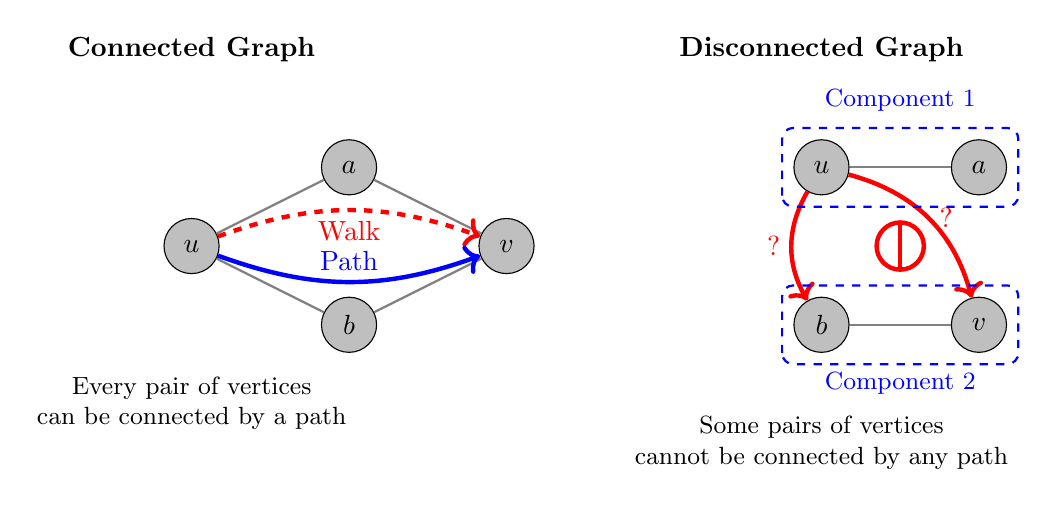
\begin{tikzpicture}[scale=1.0]
  \tikzset{
    vertex/.style={
      draw,
      circle,
      fill=lightgray,
      minimum size=0.7cm,
    },
    normaledge/.style={
      thick,
      gray,
    },
    walkpath/.style={
      ultra thick,
      red,
      dashed,
      ->,
    },
    simplepath/.style={
      ultra thick,
      blue,
      ->,
    },
    impossible/.style={
      ultra thick,
      red,
      ->,
    }
  }
  
  % Connected graph
  \begin{scope}[shift={(-4,0)}]
    \node[align=center, font=\bfseries] at (0,2.5) {Connected Graph};
    
    \node[vertex] (v1) at (0,0) {$u$};
    \node[vertex] (v2) at (2,1) {$a$};
    \node[vertex] (v3) at (2,-1) {$b$};
    \node[vertex] (v4) at (4,0) {$v$};
    
    % All edges
    \draw[normaledge] (v1) -- (v2);
    \draw[normaledge] (v1) -- (v3);
    \draw[normaledge] (v2) -- (v4);
    \draw[normaledge] (v3) -- (v4);
    
    % Walk and path
    \draw[walkpath] (v1) to[bend left=20] node[midway, below] {Walk } (v4);
    \draw[simplepath] (v1) to[bend right=20] node[midway, above] {Path} (v4);
    
    % Explanation
    \node[align=center, font=\small] at (0,-2) {
      Every pair of vertices\\can be connected by a path
    };
  \end{scope}
  
  % Disconnected graph
  \begin{scope}[shift={(4,0)}]
    \node[align=center, font=\bfseries] at (0,2.5) {Disconnected Graph};
    
    \node[vertex] (u1) at (0,1) {$u$};
    \node[vertex] (u2) at (2,1) {$a$};
    \node[vertex] (u3) at (0,-1) {$b$};
    \node[vertex] (u4) at (2,-1) {$v$};
    
    % All edges
    \draw[normaledge] (u1) -- (u2);
    \draw[normaledge] (u3) -- (u4);
    
    % Impossible paths
    \draw[impossible] (u1) to[bend right=30] node[midway, left] {?} (u3);
    \draw[impossible] (u1) to[bend left=30] node[midway, right] {?} (u4);
    \draw[red, ultra thick] (1,0) circle (0.3cm);
    \draw[red, ultra thick] (1,0.3) -- (1,-0.3);
    
    % Explanation
    \node[align=center, font=\small] at (0,-2.5) {
      Some pairs of vertices\\cannot be connected by any path
    };
    
    % Connected components highlight
    \draw[blue, dashed, rounded corners, thick] (-0.5,0.5) rectangle (2.5,1.5);
    \draw[blue, dashed, rounded corners, thick] (-0.5,-1.5) rectangle (2.5,-0.5);
    \node[blue, font=\small] at (1,1.85) {Component 1};
    \node[blue, font=\small] at (1,-1.75) {Component 2};
  \end{scope}
\end{tikzpicture}
\end{center}

% Caption for Figure 21
\vspace{0.3cm}
{\centering
\footnotesize Figure 21: Comparison of connected and disconnected graphs. In the connected graph (left), there exists at least one path between any pair of vertices, as shown by the example paths between vertices $u$ and $v$. The red dashed line represents one possible walk, while the blue solid line represents a path. In a disconnected graph (right), there exist pairs of vertices that cannot be connected by any path, as indicated by the crossed-out paths. The disconnected graph has two connected components (outlined in blue), which are maximal connected subgraphs.
\par}

\begin{proof}
Suppose vertices $u, v \in V(G)$ are the ends of a walk:
\begin{align*}
u = v_0, v_1, \ldots, v_k = v
\end{align*}
Take a shortest walk from $u$ to $v$. We can cut out any loops in the walk.
If some $v_i$ is visited more than once, say:
\begin{align*}
u \to v_i \to \ldots \to v_i \to v
\end{align*}
Then we can use the segment of the walk from $u$ to $v_i$ followed by the segment from $v_i$ to $v$:
\begin{align*}
u \to v_i \to v
\end{align*}
which is shorter, a contradiction.
So a shortest walk from $u$ to $v$ is a path.
\end{proof}

\begin{center}
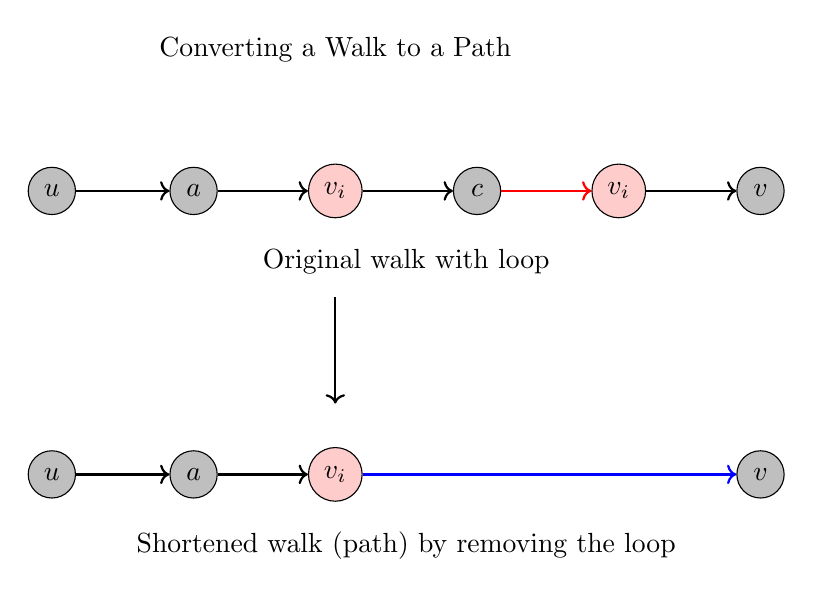
\begin{tikzpicture}[scale=0.9]
  % Proof diagram
  \node[align=center] at (0,3) {Converting a Walk to a Path};
  
  % Original walk (with loop)
  \begin{scope}[shift={(0,1)}]
    \node[draw, circle, fill=lightgray, minimum size=0.6cm] (u) at (-4,0) {$u$};
    \node[draw, circle, fill=lightgray, minimum size=0.6cm] (a) at (-2,0) {$a$};
    \node[draw, circle, fill=red!20, minimum size=0.6cm] (b) at (0,0) {$v_i$};
    \node[draw, circle, fill=lightgray, minimum size=0.6cm] (c) at (2,0) {$c$};
    \node[draw, circle, fill=red!20, minimum size=0.6cm] (b2) at (4,0) {$v_i$};
    \node[draw, circle, fill=lightgray, minimum size=0.6cm] (v) at (6,0) {$v$};
    
    \draw[->, thick] (u) -- (a);
    \draw[->, thick] (a) -- (b);
    \draw[->, thick] (b) -- (c);
    \draw[->, thick, red] (c) -- (b2);
    \draw[->, thick] (b2) -- (v);
    
    \node[align=center] at (1,-1) {Original walk with loop};
  \end{scope}
  
  \draw[->, thick] (0,-0.5) -- (0,-2);
  
  % Shortened walk (path)
  \begin{scope}[shift={(0,-3)}]
    \node[draw, circle, fill=lightgray, minimum size=0.6cm] (u) at (-4,0) {$u$};
    \node[draw, circle, fill=lightgray, minimum size=0.6cm] (a) at (-2,0) {$a$};
    \node[draw, circle, fill=red!20, minimum size=0.6cm] (b) at (0,0) {$v_i$};
    \node[draw, circle, fill=lightgray, minimum size=0.6cm] (v) at (6,0) {$v$};
    
    \draw[->, thick] (u) -- (a);
    \draw[->, thick] (a) -- (b);
    \draw[->, thick, blue] (b) -- (v);
    
    \node[align=center] at (1,-1) {Shortened walk (path) by removing the loop};
  \end{scope}
\end{tikzpicture}
\end{center}

% Caption
\vspace{0.3cm}
{\centering
\footnotesize Figure 22: Illustration of the process of converting a walk to a path by removing loops. In the original walk (top), vertex $v_i$ appears twice, creating a loop in the walk. By removing the portion of the walk between the two occurrences of $v_i$ (marked in red), we obtain a shorter walk from $u$ to $v$ that doesn't repeat any vertices (bottom), thus forming a path. This technique is fundamental for proving that if there exists a walk between two vertices in a graph, then there must also exist a path between them.
\par}

\subsubsection{More Examples of Walks, Paths, and Components}
\begin{center}
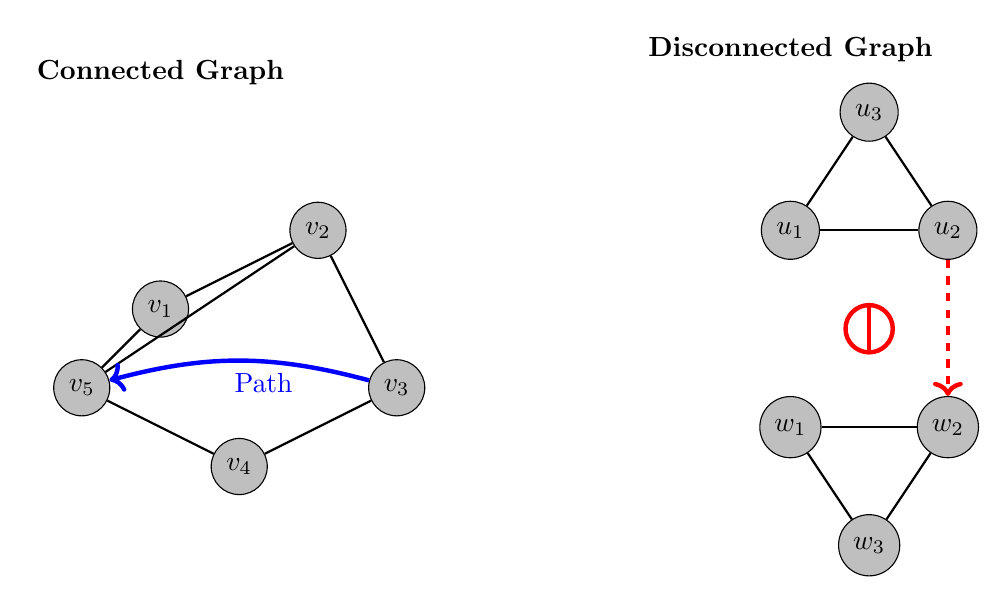
\begin{tikzpicture}[scale=1.0]
  % Connected graph
  \begin{scope}[shift={(-4,0)}]
    \node[align=center,font=\bfseries] at (0,3) {Connected Graph};
    
    % Vertices
    \node[draw, circle, fill=lightgray, minimum size=0.7cm] (v1) at (0,0) {$v_1$};
    \node[draw, circle, fill=lightgray, minimum size=0.7cm] (v2) at (2,1) {$v_2$};
    \node[draw, circle, fill=lightgray, minimum size=0.7cm] (v3) at (3,-1) {$v_3$};
    \node[draw, circle, fill=lightgray, minimum size=0.7cm] (v4) at (1,-2) {$v_4$};
    \node[draw, circle, fill=lightgray, minimum size=0.7cm] (v5) at (-1,-1) {$v_5$};
    
    % Edges
    \draw[thick] (v1) -- (v2);
    \draw[thick] (v2) -- (v3);
    \draw[thick] (v3) -- (v4);
    \draw[thick] (v4) -- (v5);
    \draw[thick] (v5) -- (v1);
    \draw[thick] (v2) -- (v5);
    
    % Highlight a path between arbitrary vertices
    \draw[->, ultra thick, blue] (v3) to[bend right=15] node[pos=0.4, below] {Path} (v5);
  \end{scope}
  
  % Disconnected graph
  \begin{scope}[shift={(4,0)}]
    \node[align=center,font=\bfseries] at (0,3.3) {Disconnected Graph};
    
    % First component
    \node[draw, circle, fill=lightgray, minimum size=0.7cm] (u1) at (0,1) {$u_1$};
    \node[draw, circle, fill=lightgray, minimum size=0.7cm] (u2) at (2,1) {$u_2$};
    \node[draw, circle, fill=lightgray, minimum size=0.7cm] (u3) at (1,2.5) {$u_3$};
    
    % Second component
    \node[draw, circle, fill=lightgray, minimum size=0.7cm] (w1) at (0,-1.5) {$w_1$};
    \node[draw, circle, fill=lightgray, minimum size=0.7cm] (w2) at (2,-1.5) {$w_2$};
    \node[draw, circle, fill=lightgray, minimum size=0.7cm] (w3) at (1,-3) {$w_3$};
    
    % Edges
    \draw[thick] (u1) -- (u2);
    \draw[thick] (u2) -- (u3);
    \draw[thick] (u3) -- (u1);
    
    \draw[thick] (w1) -- (w2);
    \draw[thick] (w2) -- (w3);
    \draw[thick] (w3) -- (w1);
    
    % Impossible path indicator
    \draw[->, ultra thick, red, dashed] (u2) -- (w2);
    \draw[red, ultra thick] (1,-0.25) circle (0.3cm);
    \draw[red, ultra thick] (1,0.05) -- (1,-0.55);
  \end{scope}
\end{tikzpicture}
\end{center}

% Caption
\vspace{0.3cm}
{\centering
\footnotesize Figure 23: Comparison of connected and disconnected graphs. The connected graph (left) has a single component where a path exists between any pair of vertices, demonstrated by the blue path from $v_3$ to $v_5$. The disconnected graph (right) contains two triangular structures that have no paths between them, as shown by the crossed-out red line. This fundamental distinction affects many graph properties, including traversability, algorithmic complexity, and network reliability.
\par}

\begin{center}
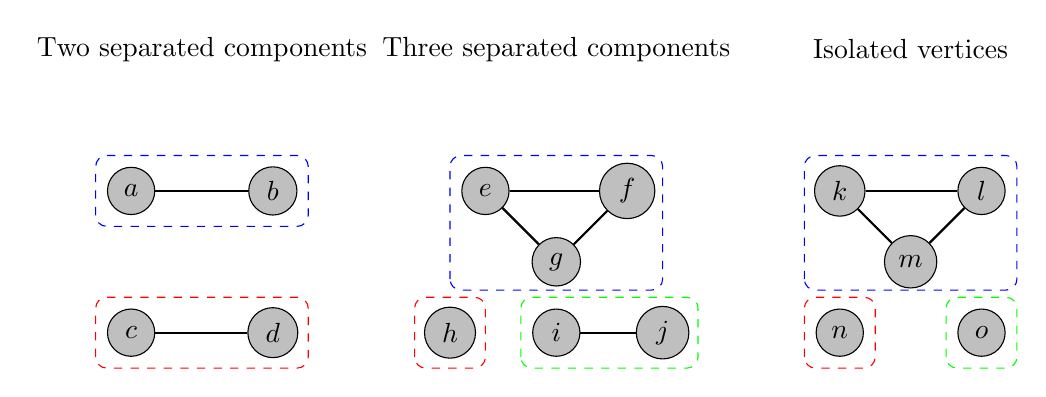
\begin{tikzpicture}[scale=0.9]
  % Various examples of disconnected graphs
  
  % Example 1: Two separated components
  \begin{scope}[shift={(-5,0)}]
    \node[align=center] at (0,3) {Two separated components};
    
    % First component
    \node[draw, circle, fill=lightgray, minimum size=0.6cm] (a1) at (-1,1) {$a$};
    \node[draw, circle, fill=lightgray, minimum size=0.6cm] (a2) at (1,1) {$b$};
    \draw[thick] (a1) -- (a2);
    
    % Second component
    \node[draw, circle, fill=lightgray, minimum size=0.6cm] (a3) at (-1,-1) {$c$};
    \node[draw, circle, fill=lightgray, minimum size=0.6cm] (a4) at (1,-1) {$d$};
    \draw[thick] (a3) -- (a4);
    
    % Component distinction
    \draw[blue, dashed, rounded corners] (-1.5,0.5) rectangle (1.5,1.5);
    \draw[red, dashed, rounded corners] (-1.5,-1.5) rectangle (1.5,-0.5);
  \end{scope}
  
  % Example 2: Three separated components
  \begin{scope}[shift={(0,0)}]
    \node[align=center] at (0,3) {Three separated components};
    
    % First component (triangle)
    \node[draw, circle, fill=lightgray, minimum size=0.6cm] (b1) at (-1,1) {$e$};
    \node[draw, circle, fill=lightgray, minimum size=0.6cm] (b2) at (1,1) {$f$};
    \node[draw, circle, fill=lightgray, minimum size=0.6cm] (b3) at (0,0) {$g$};
    \draw[thick] (b1) -- (b2);
    \draw[thick] (b2) -- (b3);
    \draw[thick] (b3) -- (b1);
    
    % Second component (single vertex)
    \node[draw, circle, fill=lightgray, minimum size=0.6cm] (b4) at (-1.5,-1) {$h$};
    
    % Third component (line)
    \node[draw, circle, fill=lightgray, minimum size=0.6cm] (b5) at (0,-1) {$i$};
    \node[draw, circle, fill=lightgray, minimum size=0.6cm] (b6) at (1.5,-1) {$j$};
    \draw[thick] (b5) -- (b6);
    
    % Component distinction
    \draw[blue, dashed, rounded corners] (-1.5,-0.4) rectangle (1.5,1.5);
    \draw[red, dashed, rounded corners] (-2,-1.5) rectangle (-1,-0.5);
    \draw[green, dashed, rounded corners] (-0.5,-1.5) rectangle (2,-0.5);
  \end{scope}
  
  % Example 3: Case with isolated vertices
  \begin{scope}[shift={(5,0)}]
    \node[align=center] at (0,3) {Isolated vertices};
    
    % Main component
    \node[draw, circle, fill=lightgray, minimum size=0.6cm] (c1) at (-1,1) {$k$};
    \node[draw, circle, fill=lightgray, minimum size=0.6cm] (c2) at (1,1) {$l$};
    \node[draw, circle, fill=lightgray, minimum size=0.6cm] (c3) at (0,0) {$m$};
    \draw[thick] (c1) -- (c2);
    \draw[thick] (c2) -- (c3);
    \draw[thick] (c3) -- (c1);
    
    % Isolated vertices
    \node[draw, circle, fill=lightgray, minimum size=0.6cm] (c4) at (-1,-1) {$n$};
    \node[draw, circle, fill=lightgray, minimum size=0.6cm] (c5) at (1,-1) {$o$};
    
    % Component distinction
    \draw[blue, dashed, rounded corners] (-1.5,-0.4) rectangle (1.5,1.5);
    \draw[red, dashed, rounded corners] (-1.5,-1.5) rectangle (-0.5,-0.5);
    \draw[green, dashed, rounded corners] (0.5,-1.5) rectangle (1.5,-0.5);
  \end{scope}
\end{tikzpicture}
\end{center}

% Caption
\vspace{0.3cm}
{\centering
\footnotesize Figure 24: Various forms of disconnected graphs. Left: A disconnected graph with two separate edge components, where each component is a single edge. Middle: A graph with three distinct components - a triangular component, a single isolated vertex, and a path component with two vertices. Right: A graph with a triangular component and two isolated vertices. Each connected component (highlighted by dashed colored rectangles) forms a maximal connected subgraph. In graph theory, isolated vertices are considered separate connected components.
\par}

\begin{center}
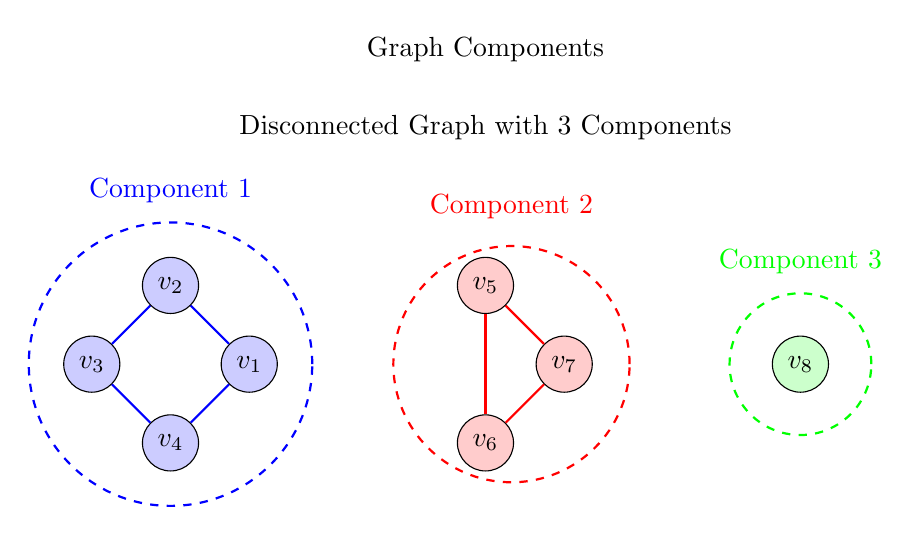
\begin{tikzpicture}[scale=1.0]
  % Disconnected graph and its components
  \node[align=center] at (0,4) {Graph Components};
  
  % Original disconnected graph
  \begin{scope}
    \node[align=center] at (0,3) {Disconnected Graph with 3 Components};
    
    % First component
    \node[draw, circle, fill=blue!20, minimum size=0.7cm] (v1) at (-3,0) {$v_1$};
    \node[draw, circle, fill=blue!20, minimum size=0.7cm] (v2) at (-4,1) {$v_2$};
    \node[draw, circle, fill=blue!20, minimum size=0.7cm] (v3) at (-5,0) {$v_3$};
    \node[draw, circle, fill=blue!20, minimum size=0.7cm] (v4) at (-4,-1) {$v_4$};
    
    % First component edges
    \draw[thick, blue] (v1) -- (v2);
    \draw[thick, blue] (v2) -- (v3);
    \draw[thick, blue] (v3) -- (v4);
    \draw[thick, blue] (v4) -- (v1);
    
    % Second component
    \node[draw, circle, fill=red!20, minimum size=0.7cm] (v5) at (0,1) {$v_5$};
    \node[draw, circle, fill=red!20, minimum size=0.7cm] (v6) at (0,-1) {$v_6$};
    \node[draw, circle, fill=red!20, minimum size=0.7cm] (v7) at (1,0) {$v_7$};
    
    % Second component edges
    \draw[thick, red] (v5) -- (v6);
    \draw[thick, red] (v6) -- (v7);
    \draw[thick, red] (v7) -- (v5);
    
    % Third component (single vertex)
    \node[draw, circle, fill=green!20, minimum size=0.7cm] (v8) at (4,0) {$v_8$};
    
    % Component emphasis (dashed circles)
    \draw[blue, dashed, thick] (-4,0) circle (1.8cm);
    \draw[red, dashed, thick] (0.33,0) circle (1.5cm);
    \draw[green, dashed, thick] (4,0) circle (0.9cm);
    
    % Component labels - positioned to avoid overlap
    \node[blue] at (-4,2.2) {Component 1};
    \node[red] at (0.33,2) {Component 2};
    \node[green] at (4,1.3) {Component 3};
  \end{scope}
\end{tikzpicture}
\end{center}

% Caption
\vspace{0.3cm}
{\centering
\footnotesize Figure 25: Illustration of a disconnected graph with three distinct components. Component 1 (blue) is a cycle graph with 4 vertices. Component 2 (red) is a triangle with 3 vertices. Component 3 (green) consists of a single isolated vertex. Each component is a maximal connected subgraph, meaning that there exists a path between any two vertices within the same component, but no path between vertices from different components. The number of components in a graph is an important invariant that affects connectivity, traversability, and many graph algorithms.
\par}

\newpage
\subsection{Chapter 1 Exercises}

\subsubsection{Easy Questions}

\begin{enumerate}
\item Define the degree of a vertex in a graph and calculate the sum of all vertex degrees in the cycle graph $C_5$.

\item Draw all possible non-isomorphic simple graphs with exactly 3 vertices.

\item Consider the following graph:
\begin{center}
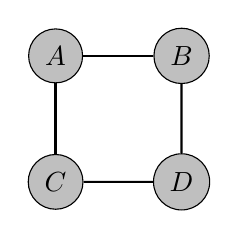
\begin{tikzpicture}[scale=0.8]
    \node[draw, circle, fill=lightgray, minimum size=0.6cm] (A) at (0,0) {$A$};
    \node[draw, circle, fill=lightgray, minimum size=0.6cm] (B) at (2,0) {$B$};
    \node[draw, circle, fill=lightgray, minimum size=0.6cm] (C) at (0,-2) {$C$};
    \node[draw, circle, fill=lightgray, minimum size=0.6cm] (D) at (2,-2) {$D$};
    
    \draw[thick] (A) -- (B);
    \draw[thick] (A) -- (C);
    \draw[thick] (B) -- (D);
    \draw[thick] (C) -- (D);
\end{tikzpicture}
\end{center}
List all paths from vertex $A$ to vertex $D$.

\item What is the difference between a walk and a path in a graph? Give an example of a walk that is not a path.

\item For each of the following graphs, determine if it is connected or disconnected:
\begin{itemize}
    \item A star graph $S_6$
    \item A path graph $P_4$
    \item A graph with vertices $\{a,b,c,d\}$ and edges $\{\{a,b\}, \{c,d\}\}$
\end{itemize}
\end{enumerate}

\subsubsection{Intermediate Questions}

\begin{enumerate}[resume]
\item Draw a graph with degree sequence $(3,3,2,2,2,0)$. Is there more than one non-isomorphic graph with this degree sequence?

\item Prove that a connected graph with $n$ vertices must have at least $n-1$ edges.

\item Consider a graph $G$ with vertex set $V = \{1,2,3,4,5,6\}$ and edges 
$\{1,2\}$, $\{1,5\}$, $\{2,3\}$, $\{2,5\}$,\\
$\{3,4\}$, $\{4,5\}$, $\{4,6\}$, $\{5,6\}$.
\begin{center}
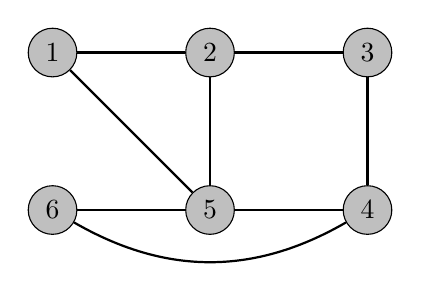
\begin{tikzpicture}[scale=1.0]
    \node[draw, circle, fill=lightgray, minimum size=0.6cm] (1) at (0,0) {$1$};
    \node[draw, circle, fill=lightgray, minimum size=0.6cm] (2) at (2,0) {$2$};
    \node[draw, circle, fill=lightgray, minimum size=0.6cm] (3) at (4,0) {$3$};
    \node[draw, circle, fill=lightgray, minimum size=0.6cm] (4) at (4,-2) {$4$};
    \node[draw, circle, fill=lightgray, minimum size=0.6cm] (5) at (2,-2) {$5$};
    \node[draw, circle, fill=lightgray, minimum size=0.6cm] (6) at (0,-2) {$6$};
    
    \draw[thick] (1) -- (2);
    \draw[thick] (1) -- (5);
    \draw[thick] (2) -- (3);
    \draw[thick] (2) -- (5);
    \draw[thick] (3) -- (4);
    \draw[thick] (4) -- (5);
    \draw[thick] (4) to[bend left=30] (6); % Bent edge to avoid confusion
    \draw[thick] (5) -- (6);
\end{tikzpicture}
\end{center}
\begin{itemize}
    \item Find an induced subgraph with vertex set $\{1,2,5,6\}$
    \item Find a spanning subgraph with exactly 6 edges
\end{itemize}

\item The Petersen graph is shown in your textbook (Figure 11). Find the longest path in this graph. Prove that your path is indeed the longest possible.

\item Show that any graph with at least two vertices must have at least two vertices with the same degree.

\end{enumerate}

\subsubsection{Hard Questions}

\begin{enumerate}[resume]
\item Prove that if $G$ is a simple graph with $n$ vertices and more than $\frac{(n-1)(n-2)}{2}$ edges, then $G$ must be connected.

\item Let $G$ be a graph with $n$ vertices. If each vertex has degree at least $\frac{n-1}{2}$, prove that $G$ is connected.

\item A graph is called bipartite if its vertices can be divided into two disjoint sets such that every edge connects a vertex in the first set to one in the second set.
\begin{itemize}
    \item Prove that a graph is bipartite if and only if it contains no cycles of odd length.
    \item Which of the following graphs are bipartite: $C_4$, $C_5$, $K_{3,3}$, the Petersen graph?
\end{itemize}

\item Design a graph that:
\begin{itemize}
    \item Has exactly 8 vertices
    \item Is connected
    \item Has exactly 3 vertices of degree 3, and the rest of degree 2
    \item Contains exactly one cycle of length 4 and one cycle of length 5
\end{itemize}

\item Consider the hypercube graph $Q_4$.
\begin{itemize}
    \item How many vertices and edges does $Q_4$ have?
    \item What is the degree of each vertex?
    \item Devise an algorithm to determine if there exists a path of length exactly $k$ between any two vertices in $Q_4$.
\end{itemize}
\end{enumerate}

\subsubsection{Questions with Diagrams}

\begin{enumerate}[resume]
\item For the graph below, identify:
\begin{itemize}
    \item All isolated vertices
    \item All pendant vertices
    \item The degree sequence
    \item The number of connected components
\end{itemize}

\begin{center}
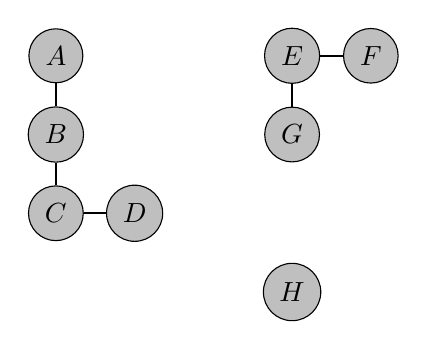
\begin{tikzpicture}[scale=1.0]
    \node[draw, circle, fill=lightgray, minimum size=0.6cm] (A) at (0,0) {$A$};
    \node[draw, circle, fill=lightgray, minimum size=0.6cm] (B) at (0,-1) {$B$};
    \node[draw, circle, fill=lightgray, minimum size=0.6cm] (C) at (0,-2) {$C$};
    \node[draw, circle, fill=lightgray, minimum size=0.6cm] (D) at (1,-2) {$D$};
    \node[draw, circle, fill=lightgray, minimum size=0.6cm] (E) at (3,0) {$E$};
    \node[draw, circle, fill=lightgray, minimum size=0.6cm] (F) at (4,0) {$F$};
    \node[draw, circle, fill=lightgray, minimum size=0.6cm] (G) at (3,-1) {$G$};
    \node[draw, circle, fill=lightgray, minimum size=0.6cm] (H) at (3,-3) {$H$};
    
    \draw[thick] (A) -- (B);
    \draw[thick] (B) -- (C);
    \draw[thick] (C) -- (D);
    \draw[thick] (E) -- (F);
    \draw[thick] (E) -- (G);
\end{tikzpicture}
\end{center}

\item Draw all possible spanning trees of the following graph:

\begin{center}
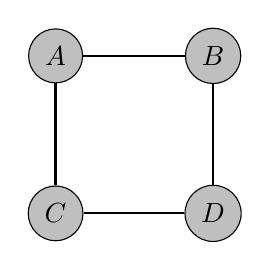
\begin{tikzpicture}[scale=1.0]
    \node[draw, circle, fill=lightgray, minimum size=0.6cm] (A) at (0,0) {$A$};
    \node[draw, circle, fill=lightgray, minimum size=0.6cm] (B) at (2,0) {$B$};
    \node[draw, circle, fill=lightgray, minimum size=0.6cm] (C) at (0,-2) {$C$};
    \node[draw, circle, fill=lightgray, minimum size=0.6cm] (D) at (2,-2) {$D$};
    
    \draw[thick] (A) -- (B);
    \draw[thick] (A) -- (C);
    \draw[thick] (B) -- (D);
    \draw[thick] (C) -- (D);
\end{tikzpicture}
\end{center}

\item Consider the graph $G$ shown below:

\begin{center}
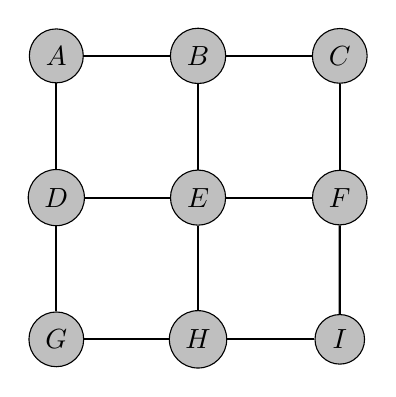
\begin{tikzpicture}[scale=0.9]
    \node[draw, circle, fill=lightgray, minimum size=0.6cm] (A) at (0,0) {$A$};
    \node[draw, circle, fill=lightgray, minimum size=0.6cm] (B) at (2,0) {$B$};
    \node[draw, circle, fill=lightgray, minimum size=0.6cm] (C) at (4,0) {$C$};
    \node[draw, circle, fill=lightgray, minimum size=0.6cm] (D) at (0,-2) {$D$};
    \node[draw, circle, fill=lightgray, minimum size=0.6cm] (E) at (2,-2) {$E$};
    \node[draw, circle, fill=lightgray, minimum size=0.6cm] (F) at (4,-2) {$F$};
    \node[draw, circle, fill=lightgray, minimum size=0.6cm] (G) at (0,-4) {$G$};
    \node[draw, circle, fill=lightgray, minimum size=0.6cm] (H) at (2,-4) {$H$};
    \node[draw, circle, fill=lightgray, minimum size=0.6cm] (I) at (4,-4) {$I$};
    
    \draw[thick] (A) -- (B);
    \draw[thick] (B) -- (C);
    \draw[thick] (A) -- (D);
    \draw[thick] (B) -- (E);
    \draw[thick] (C) -- (F);
    \draw[thick] (D) -- (E);
    \draw[thick] (E) -- (F);
    \draw[thick] (D) -- (G);
    \draw[thick] (E) -- (H);
    \draw[thick] (F) -- (I);
    \draw[thick] (G) -- (H);
    \draw[thick] (H) -- (I);
\end{tikzpicture}
\end{center}

\begin{enumerate}[label=\alph*)]
    \item Draw an induced subgraph $G[\{A,B,D,E\}]$
    \item Find a subgraph that is not an induced subgraph
    \item Draw a spanning subgraph that is a tree
    \item What is the maximum number of edges that can be removed while keeping the graph connected?
\end{enumerate}

\item In the wheel graph $W_6$ (shown below), find:
\begin{itemize}
    \item The shortest path from any outer vertex to the vertex diametrically opposite on the cycle
    \item The number of distinct cycles of length 3
    \item The number of distinct cycles of length 4
\end{itemize}

\begin{center}
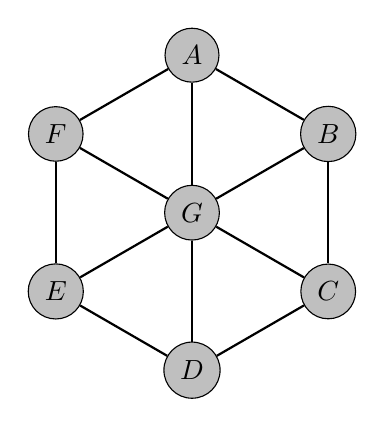
\begin{tikzpicture}[scale=1.0]
    \node[draw, circle, fill=lightgray, minimum size=0.6cm] (G) at (0,0) {$G$};
    \node[draw, circle, fill=lightgray, minimum size=0.6cm] (A) at (0,2) {$A$};
    \node[draw, circle, fill=lightgray, minimum size=0.6cm] (B) at (1.73,1) {$B$};
    \node[draw, circle, fill=lightgray, minimum size=0.6cm] (C) at (1.73,-1) {$C$};
    \node[draw, circle, fill=lightgray, minimum size=0.6cm] (D) at (0,-2) {$D$};
    \node[draw, circle, fill=lightgray, minimum size=0.6cm] (E) at (-1.73,-1) {$E$};
    \node[draw, circle, fill=lightgray, minimum size=0.6cm] (F) at (-1.73,1) {$F$};
    
    \draw[thick] (A) -- (B);
    \draw[thick] (B) -- (C);
    \draw[thick] (C) -- (D);
    \draw[thick] (D) -- (E);
    \draw[thick] (E) -- (F);
    \draw[thick] (F) -- (A);
    
    \draw[thick] (G) -- (A);
    \draw[thick] (G) -- (B);
    \draw[thick] (G) -- (C);
    \draw[thick] (G) -- (D);
    \draw[thick] (G) -- (E);
    \draw[thick] (G) -- (F);
\end{tikzpicture}
\end{center}

\item Given the Petersen graph:
\begin{center}
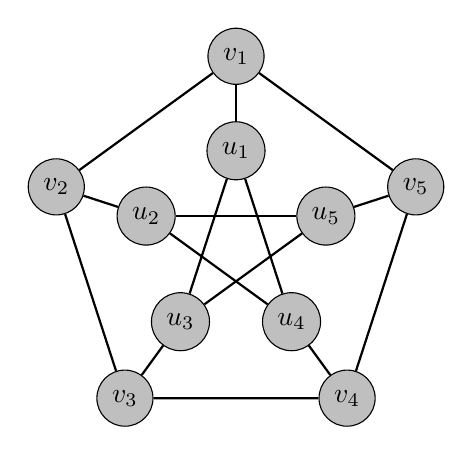
\begin{tikzpicture}[scale=1.2]
  % Outer pentagon
  \foreach \i in {1,...,5} {
    \node[draw, circle, fill=lightgray, minimum size=0.6cm] (v\i) at ({72*(\i-1)+90}:2) {$v_{\i}$};
  }
  
  % Inner pentagon
  \foreach \i in {1,...,5} {
    \node[draw, circle, fill=lightgray, minimum size=0.6cm] (u\i) at ({72*(\i-1)+90}:1) {$u_{\i}$};
  }
  
  % Connect outer pentagon
  \foreach \i in {1,...,5} {
    \pgfmathtruncatemacro{\j}{mod(\i,5)+1}
    \draw[thick] (v\i) -- (v\j);
  }
  
  % Connect inner to outer
  \foreach \i in {1,...,5} {
    \draw[thick] (v\i) -- (u\i);
  }
  
  % Connect inner pentagon in star pattern
  \foreach \i in {1,...,5} {
    \pgfmathtruncatemacro{\j}{mod(\i+1,5)+1}
    \draw[thick] (u\i) -- (u\j);
  }
\end{tikzpicture}
\end{center}

\begin{enumerate}[label=\alph*)]
    \item Prove that it does not contain a cycle of length 3
    \item Find all cycles of length 5
    \item Show that the graph is not bipartite
\end{enumerate}

\end{enumerate}


\section{Eulerian Graphs}

\subsection{Trails and Tours}

\begin{definition}
A trail in a graph is a sequence of vertices:
\begin{align*}
v_1, v_2, \ldots, v_n
\end{align*}
such that $\{v_i, v_{i+1}\} \in E(G)$ and no edge appears twice. Unlike a path, a trail may visit the same vertex multiple times, but it cannot use the same edge more than once.
\end{definition}

\begin{definition}
A tour is a trail $v_1, v_2, \ldots, v_n$ with $v_n = v_1$. That is, a tour is a closed trail that starts and ends at the same vertex. A tour is also sometimes called a circuit.
\end{definition}

\begin{definition}
An Eulerian trail is a trail that traverses every edge of the graph exactly once.
\end{definition}

\begin{definition}
An Eulerian tour (or Eulerian circuit) is a tour that traverses every edge of the graph exactly once.
\end{definition}

\begin{theorem}
Let $G$ be a connected graph (or multigraph), and let $u, v \in V(G)$. Then:
\begin{enumerate}
\item The graph has an Eulerian tour if and only if all vertices have even degree.
\item The graph has an Eulerian trail from $u$ to $v$ if and only if $u$ and $v$ have odd degree and all other vertices have even degree.
\end{enumerate}
\end{theorem}

\begin{figure}[ht]
\centering
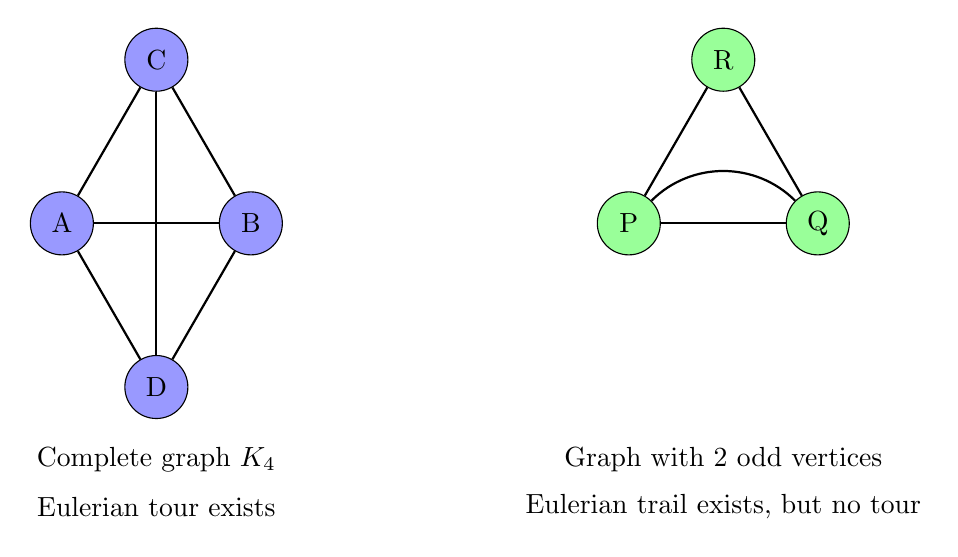
\begin{tikzpicture}[scale=1.2]
    % Example 1: Graph with Eulerian Tour
    \begin{scope}[shift={(-3,0)}]
        % Vertices
        \node[circle, draw, fill=blue!40, minimum size=0.8cm] (A) at (0,0) {A};
        \node[circle, draw, fill=blue!40, minimum size=0.8cm] (B) at (2,0) {B};
        \node[circle, draw, fill=blue!40, minimum size=0.8cm] (C) at (1,1.732) {C};
        \node[circle, draw, fill=blue!40, minimum size=0.8cm] (D) at (1,-1.732) {D};
        
        % Edges
        \draw[thick] (A) -- (B);
        \draw[thick] (A) -- (C);
        \draw[thick] (A) -- (D);
        \draw[thick] (B) -- (C);
        \draw[thick] (B) -- (D);
        \draw[thick] (C) -- (D);
        
        \node at (1,-2.5) {Complete graph $K_4$};
        \node at (1,-3) {Eulerian tour exists};
    \end{scope}
    
    % Example 2: Graph with Eulerian Trail but no Tour
    \begin{scope}[shift={(3,0)}]
        % Vertices
        \node[circle, draw, fill=green!40, minimum size=0.8cm] (P) at (0,0) {P};
        \node[circle, draw, fill=green!40, minimum size=0.8cm] (Q) at (2,0) {Q};
        \node[circle, draw, fill=green!40, minimum size=0.8cm] (R) at (1,1.732) {R};
        
        % Edges
        \draw[thick] (P) -- (Q);
        \draw[thick] (P) -- (R);
        \draw[thick] (Q) -- (R);
        \draw[thick] (P) to[bend left=45] (Q);
        
        \node at (1,-2.5) {Graph with 2 odd vertices};
        \node at (1,-3) {Eulerian trail exists, but no tour};
    \end{scope}
\end{tikzpicture}

\vspace{0.3cm}
{\centering
\small Figure 26: Example graphs illustrating Eulerian concepts. Left: Complete graph $K_4$ where all vertices have degree 3 (odd). Although it doesn't have an Eulerian tour, it does have an Eulerian trail. Right: A graph with exactly two odd-degree vertices (P and Q) that has an Eulerian trail but no Eulerian tour.
\par}
\end{figure}

\begin{figure}[ht]
\centering
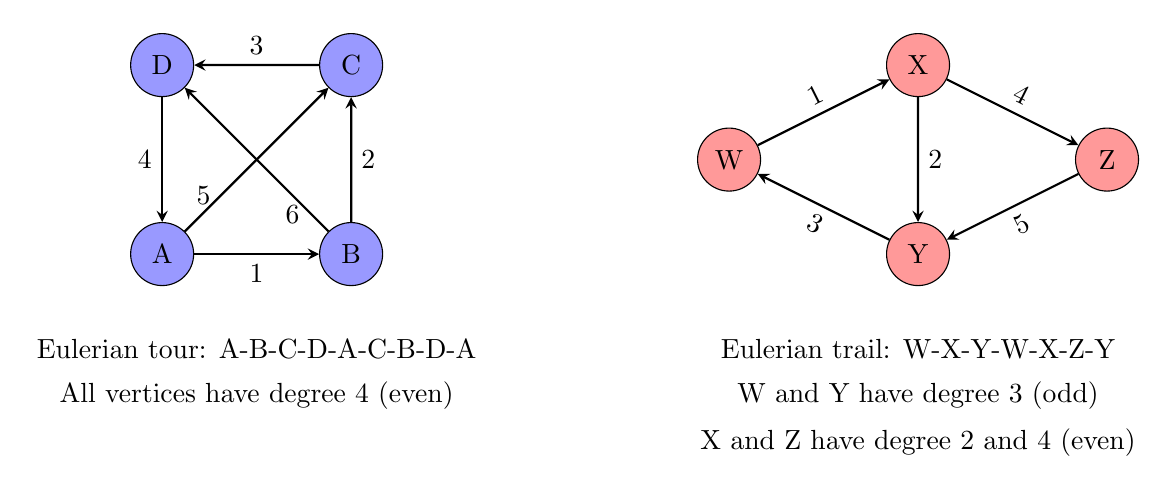
\begin{tikzpicture}[scale=1.2]
    % Example 3: Graph with Eulerian tour - showing the tour
    \begin{scope}[shift={(-2.5,0)}]
        % Vertices
        \node[circle, draw, fill=blue!40, minimum size=0.8cm] (A) at (0,0) {A};
        \node[circle, draw, fill=blue!40, minimum size=0.8cm] (B) at (2,0) {B};
        \node[circle, draw, fill=blue!40, minimum size=0.8cm] (C) at (2,2) {C};
        \node[circle, draw, fill=blue!40, minimum size=0.8cm] (D) at (0,2) {D};
        
        % Edges with directed arrows showing an Eulerian tour
        \draw[thick, ->, >=stealth] (A) -- node[below] {1} (B);
        \draw[thick, ->, >=stealth] (B) -- node[right] {2} (C);
        \draw[thick, ->, >=stealth] (C) -- node[above] {3} (D);
        \draw[thick, ->, >=stealth] (D) -- node[left] {4} (A);
        \draw[thick, ->, >=stealth] (A) -- node[near start, left] {5} (C);
        \draw[thick, ->, >=stealth] (B) -- node[near start, below] {6} (D);
        
        \node at (1,-1) {Eulerian tour: A-B-C-D-A-C-B-D-A};
        \node at (1,-1.5) {All vertices have degree 4 (even)};
    \end{scope}
    
    % Example 4: Graph with Eulerian trail but no tour - showing the trail
    \begin{scope}[shift={(3.5,0)}]
        % Vertices
        \node[circle, draw, fill=red!40, minimum size=0.8cm] (W) at (0,1) {W};
        \node[circle, draw, fill=red!40, minimum size=0.8cm] (X) at (2,2) {X};
        \node[circle, draw, fill=red!40, minimum size=0.8cm] (Y) at (2,0) {Y};
        \node[circle, draw, fill=red!40, minimum size=0.8cm] (Z) at (4,1) {Z};
        
        % Edges with directed arrows showing an Eulerian trail
        \draw[thick, ->, >=stealth] (W) -- node[above, sloped] {1} (X);
        \draw[thick, ->, >=stealth] (X) -- node[right] {2} (Y);
        \draw[thick, ->, >=stealth] (Y) -- node[below, sloped] {3} (W);
        \draw[thick, ->, >=stealth] (X) -- node[above, sloped] {4} (Z);
        \draw[thick, ->, >=stealth] (Z) -- node[below, sloped] {5} (Y);
        
        \node at (2,-1) {Eulerian trail: W-X-Y-W-X-Z-Y};
        \node at (2,-1.5) {W and Y have degree 3 (odd)};
        \node at (2,-2) {X and Z have degree 2 and 4 (even)};
    \end{scope}
\end{tikzpicture}

\vspace{0.3cm}
{\centering
\small Figure 27: Explicit examples of Eulerian tours and trails. Left: A graph where every vertex has even degree (4), with a complete Eulerian tour shown by numbered edges. The tour visits every edge exactly once and returns to the starting vertex A. Right: A graph with exactly two odd-degree vertices (W and Y), showing an Eulerian trail that traverses every edge exactly once but doesn't form a closed circuit.
\par}
\end{figure}

\begin{proof}[Proof of (1)]
$(\Rightarrow)$ Suppose there is an Eulerian tour $C = v_1, v_2, \ldots, v_m, v_1$. We prove all vertices have even degree by induction on $|E(G)|$.

Base case: $|E(G)| = 1$. The Eulerian tour is $v_1, v_1$, so $d(v_1) = 2$.

Suppose the strong induction statement is true for all graphs with fewer than $m$ edges.
Let $C = v_1, v_2, \ldots, v_m, v_1$ be an Eulerian tour in $G$ with $m$ edges.
Let $j = \min\{i > 1 : v_i = v_j \text{ for some } j < i\}$.

If $j = m+1$, then the entire tour is a simple cycle with $m$ edges, so every vertex has degree 2.

If $j < m+1$:
\begin{itemize}
\item Remove all edges $\{v_1, v_2\}, \{v_2, v_3\}, \ldots, \{v_{j-1}, v_j\}$
\end{itemize}

By induction, the remaining edges form an Eulerian tour $v_j, v_{j+1}, \ldots, v_m, v_1$, so all vertices in this subgraph have even degree.
Also, $C' = v_1, v_2, \ldots, v_j$ is also an Eulerian tour in its subgraph, so all those vertices have even degree.
Therefore, all vertices in the original graph have even degree.

$(\Leftarrow)$ Let $C = v_1, v_2, \ldots, v_n$ be a longest trail in the graph.

Case 1: Suppose $v_n \neq v_1$.
Since $v_n$ has even degree, we know an edge $\{v_n, v_{n+1}\}$ not in the trail exists.
Now $C' = v_1, v_2, \ldots, v_n, v_{n+1}$ is a longer trail, a contradiction.

Case 2: $v_n = v_1$.
Since $G$ is connected, all edges must be used by the trail.
Otherwise, relabel the trail as $v'_1, v'_2, \ldots, v'_{n-1}, v'_n = v'_1$.
We can add $\{v'_i, v'_{n+1}\}$ to create a longer trail, contradiction.
Therefore, the graph has an Eulerian tour.
\end{proof}

\begin{figure}[ht]
\centering
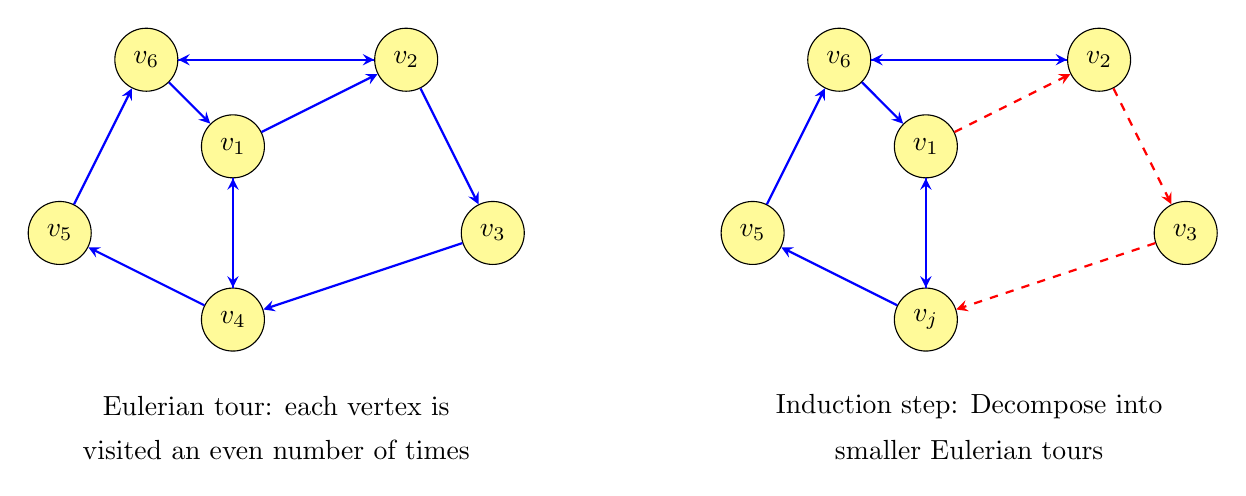
\begin{tikzpicture}[scale=1.1]
    % Visual for the forward direction of the proof
    \begin{scope}[shift={(-4,0)}]
        % Original graph
        \node[circle, draw, fill=yellow!40, minimum size=0.8cm] (A) at (0,0) {$v_1$};
        \node[circle, draw, fill=yellow!40, minimum size=0.8cm] (B) at (2,1) {$v_2$};
        \node[circle, draw, fill=yellow!40, minimum size=0.8cm] (C) at (3,-1) {$v_3$};
        \node[circle, draw, fill=yellow!40, minimum size=0.8cm] (D) at (0,-2) {$v_4$};
        \node[circle, draw, fill=yellow!40, minimum size=0.8cm] (E) at (-2,-1) {$v_5$};
        \node[circle, draw, fill=yellow!40, minimum size=0.8cm] (F) at (-1,1) {$v_6$};
        
        % Eulerian tour - directed arrows
        \draw[thick, ->, >=stealth, blue] (A) -- (B);
        \draw[thick, ->, >=stealth, blue] (B) -- (C);
        \draw[thick, ->, >=stealth, blue] (C) -- (D);
        \draw[thick, ->, >=stealth, blue] (D) -- (E);
        \draw[thick, ->, >=stealth, blue] (E) -- (F);
        \draw[thick, ->, >=stealth, blue] (F) -- (A);
        \draw[thick, ->, >=stealth, blue] (A) -- (D);
        \draw[thick, ->, >=stealth, blue] (D) -- (A);
        \draw[thick, ->, >=stealth, blue] (B) -- (F);
        \draw[thick, ->, >=stealth, blue] (F) -- (B);

        \node at (0.5,-3) {Eulerian tour: each vertex is};
        \node at (0.5,-3.5) {visited an even number of times};
    \end{scope}
    
    % Visual for the induction step - decomposition
    \begin{scope}[shift={(4,0)}]
        % Original graph structure
        \node[circle, draw, fill=yellow!40, minimum size=0.8cm] (A) at (0,0) {$v_1$};
        \node[circle, draw, fill=yellow!40, minimum size=0.8cm] (B) at (2,1) {$v_2$};
        \node[circle, draw, fill=yellow!40, minimum size=0.8cm] (C) at (3,-1) {$v_3$};
        \node[circle, draw, fill=yellow!40, minimum size=0.8cm] (D) at (0,-2) {$v_j$};
        \node[circle, draw, fill=yellow!40, minimum size=0.8cm] (E) at (-2,-1) {$v_5$};
        \node[circle, draw, fill=yellow!40, minimum size=0.8cm] (F) at (-1,1) {$v_6$};
        
        % First cycle (removed in induction)
        \draw[thick, ->, >=stealth, red, dashed] (A) -- (B);
        \draw[thick, ->, >=stealth, red, dashed] (B) -- (C);
        \draw[thick, ->, >=stealth, red, dashed] (C) -- (D);
        
        % Second cycle (remaining after removal)
        \draw[thick, ->, >=stealth, blue] (D) -- (E);
        \draw[thick, ->, >=stealth, blue] (E) -- (F);
        \draw[thick, ->, >=stealth, blue] (F) -- (A);
        \draw[thick, ->, >=stealth, blue] (A) -- (D);
        \draw[thick, ->, >=stealth, blue] (D) -- (A);
        \draw[thick, ->, >=stealth, blue] (B) -- (F);
        \draw[thick, ->, >=stealth, blue] (F) -- (B);
        
        \node at (0.5,-3) {Induction step: Decompose into};
        \node at (0.5,-3.5) {smaller Eulerian tours};
    \end{scope}
\end{tikzpicture}

\vspace{0.3cm}
{\centering
\small Figure 28: Visualization of the forward direction proof - showing why Eulerian tours imply even degrees. Left: A graph with an Eulerian tour (blue arrows) where each vertex must be visited and departed from an equal number of times, giving each vertex an even degree. Right: The induction step showing how an Eulerian tour can be decomposed into smaller Eulerian subcircuits.
\par}
\end{figure}

\begin{figure}[ht]
\centering
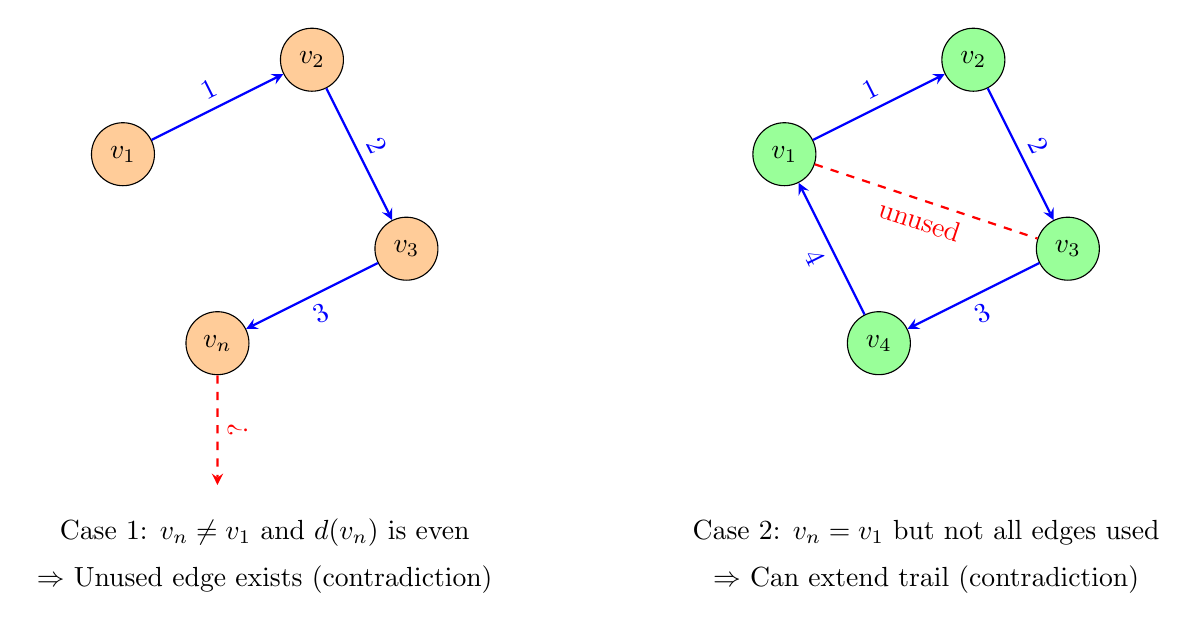
\begin{tikzpicture}[scale=1.2]
    % Case 1 visualization - trail does not end at starting vertex
    \begin{scope}[shift={(-3.5,0)}]
        % Vertices
        \node[circle, draw, fill=orange!40, minimum size=0.8cm] (A) at (0,0) {$v_1$};
        \node[circle, draw, fill=orange!40, minimum size=0.8cm] (B) at (2,1) {$v_2$};
        \node[circle, draw, fill=orange!40, minimum size=0.8cm] (C) at (3,-1) {$v_3$};
        \node[circle, draw, fill=orange!40, minimum size=0.8cm] (D) at (1,-2) {$v_n$};
        
        % Existing trail
        \draw[thick, ->, >=stealth, blue] (A) -- node[above, sloped] {1} (B);
        \draw[thick, ->, >=stealth, blue] (B) -- node[above, sloped] {2} (C);
        \draw[thick, ->, >=stealth, blue] (C) -- node[below, sloped] {3} (D);
        
        % Unused edge from v_n (must exist if degree is even)
        \draw[thick, ->, >=stealth, red, dashed] (D) -- node[below, sloped] {?} (1,-3.5);
        
        \node at (1.5,-4) {Case 1: $v_n \neq v_1$ and $d(v_n)$ is even};
        \node at (1.5,-4.5) {$\Rightarrow$ Unused edge exists (contradiction)};
    \end{scope}
    
    % Case 2 visualization - tour that doesn't use all edges
    \begin{scope}[shift={(3.5,0)}]
        % Vertices
        \node[circle, draw, fill=green!40, minimum size=0.8cm] (A) at (0,0) {$v_1$};
        \node[circle, draw, fill=green!40, minimum size=0.8cm] (B) at (2,1) {$v_2$};
        \node[circle, draw, fill=green!40, minimum size=0.8cm] (C) at (3,-1) {$v_3$};
        \node[circle, draw, fill=green!40, minimum size=0.8cm] (D) at (1,-2) {$v_4$};
        
        % Existing tour edges
        \draw[thick, ->, >=stealth, blue] (A) -- node[above, sloped] {1} (B);
        \draw[thick, ->, >=stealth, blue] (B) -- node[above, sloped] {2} (C);
        \draw[thick, ->, >=stealth, blue] (C) -- node[below, sloped] {3} (D);
        \draw[thick, ->, >=stealth, blue] (D) -- node[below, sloped] {4} (A);
        
        % Unused edge (contradiction in connected graph)
        \draw[thick, red, dashed] (A) -- node[below, sloped] {unused} (C);
        
        \node at (1.5,-4) {Case 2: $v_n = v_1$ but not all edges used};
        \node at (1.5,-4.5) {$\Rightarrow$ Can extend trail (contradiction)};
    \end{scope}
\end{tikzpicture}

\vspace{0.3cm}
{\centering
\small Figure 29: Visualization of the reverse direction proof - showing why even degrees imply Eulerian tours. Left: If the longest trail doesn't end at its starting point and the final vertex has even degree, an unused edge must exist (contradiction). Right: If the trail forms a tour but doesn't use all edges, the graph has another edge that could extend the tour (contradiction).
\par}
\end{figure}

\begin{proof}[Proof of (2)]
$(\Rightarrow)$ Suppose $G$ has an Eulerian trail from $u$ to $v$ with $u \neq v$. Add an edge $e$ between $u$ and $v$. The resulting graph $G' = G \cup \{e\}$ has an Eulerian tour. By part (1), all vertices in $G'$ have even degree.

In the original graph $G$, the degrees of $u$ and $v$ are both reduced by 1, making them odd, while all other vertices maintain their even degree.

$(\Leftarrow)$ Suppose $u$ and $v$ have odd degree, and all other vertices have even degree. Add an edge $e$ between $u$ and $v$. In the resulting graph $G' = G \cup \{e\}$, all vertices now have even degree.

By part (1), $G'$ has an Eulerian tour. This tour must use the edge $e$ at some point. Remove $e$ from the tour, and we obtain an Eulerian trail in $G$ from $u$ to $v$.
\end{proof}

\begin{figure}[ht]
\centering
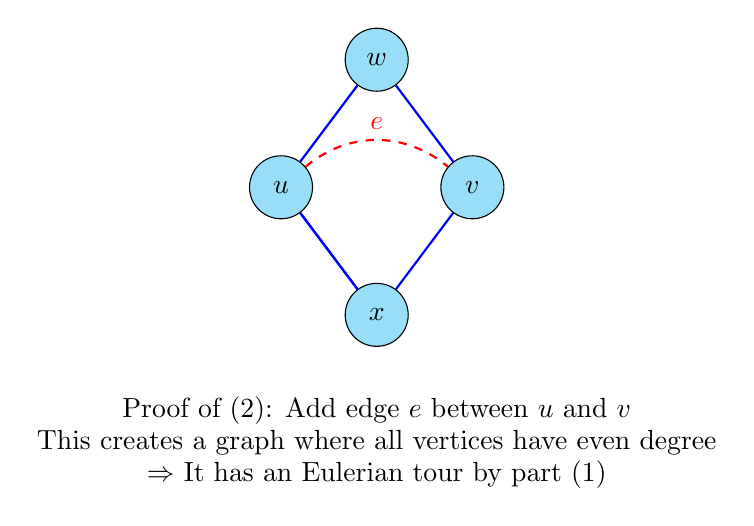
\begin{tikzpicture}[scale=0.81]
    % Graph with Eulerian trail
    \begin{scope}[shift={(0,0)}]
        % Vertices
        \node[circle, draw, fill=cyan!40, minimum size=0.8cm] (A) at (0,0) {$u$};
        \node[circle, draw, fill=cyan!40, minimum size=0.8cm] (B) at (3,0) {$v$};
        \node[circle, draw, fill=cyan!40, minimum size=0.8cm] (C) at (1.5,2) {$w$};
        \node[circle, draw, fill=cyan!40, minimum size=0.8cm] (D) at (1.5,-2) {$x$};
        
        % Original graph edges - Eulerian trail
        \draw[thick, blue] (A) -- (C);
        \draw[thick, blue] (C) -- (B);
        \draw[thick, blue] (B) -- (D);
        \draw[thick, blue] (D) -- (A);
        \draw[thick, blue] (A) -- (D);
        
        % Additional edge to create Eulerian tour
        \draw[thick, red, dashed] (A) to[bend left=40] node[above] {$e$} (B);
        
        \node at (1.5,-3.5) {Proof of (2): Add edge $e$ between $u$ and $v$};
        \node at (1.5,-4) {This creates a graph where all vertices have even degree};
        \node at (1.5,-4.5) {$\Rightarrow$ It has an Eulerian tour by part (1)};
    \end{scope}
\end{tikzpicture}

\vspace{0.3cm}
{\centering
\small Figure 30: Visualization of the proof for part (2) - Converting between Eulerian trails and tours. By adding a new edge $e$ (red dashed line) between the two odd-degree vertices $u$ and $v$, we transform the graph into one where every vertex has even degree. This creates a graph with an Eulerian tour, and removing edge $e$ gives us the original Eulerian trail.
\par}
\end{figure}

% Fleury's Algorithm - Figure Descriptions in LaTeX

\setcounter{figure}{30} % This sets the figure counter to 30, so the next figure will be 31

\begin{figure}[p]
{\centering
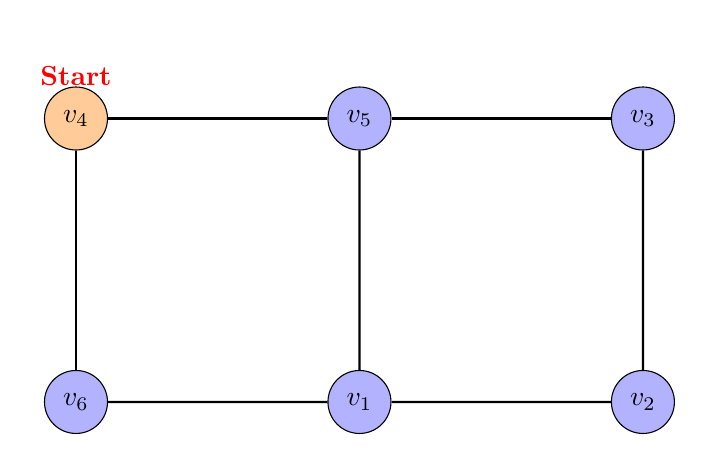
\begin{tikzpicture}[scale=1.8, 
    every node/.style={circle, draw, minimum size=0.8cm}]
    % Vertices
    \node[fill=orange!40] (v4) at (0,0) {$v_4$};
    \node[fill=blue!30] (v5) at (2,0) {$v_5$};
    \node[fill=blue!30] (v3) at (4,0) {$v_3$};
    \node[fill=blue!30] (v6) at (0,-2) {$v_6$};
    \node[fill=blue!30] (v1) at (2,-2) {$v_1$};
    \node[fill=blue!30] (v2) at (4,-2) {$v_2$};
    
    % Edges
    \draw[thick] (v4) -- (v5);
    \draw[thick] (v5) -- (v3);
    \draw[thick] (v4) -- (v6);
    \draw[thick] (v6) -- (v1);
    \draw[thick] (v1) -- (v2);
    \draw[thick] (v2) -- (v3);
    \draw[thick] (v1) -- (v5);
    
    % Start marker
    \node[text=red, font=\bfseries, draw=none, fill=none, minimum size=0cm] at (0,0.3) {Start};
\end{tikzpicture}
\par}
{\centering
\small Figure 31: Graph for applying Fleury's Algorithm. This figure displays the initial connected graph with six vertices labeled $v_1$ through $v_6$ arranged in a rectangular pattern. Vertex $v_4$ is highlighted in orange as the starting point, indicated by the red ``Start'' label. The graph has seven edges connecting the vertices in a way that allows for an Eulerian trail.
\par}
\end{figure}

\begin{figure}[p]
{\centering
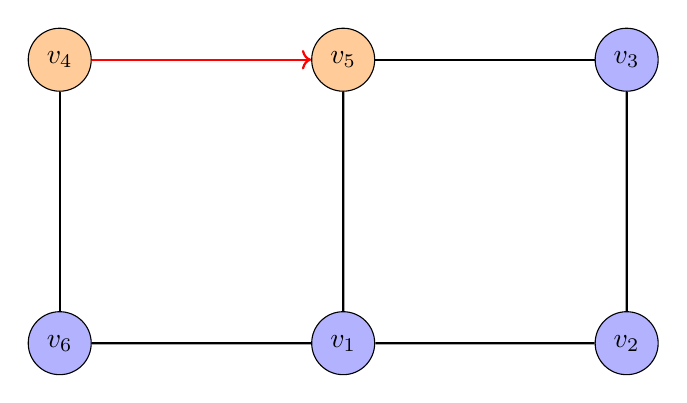
\begin{tikzpicture}[scale=1.8, 
    every node/.style={circle, draw, minimum size=0.8cm}]
    % Vertices - Step 1
    \node[fill=orange!40] (v4) at (0,0) {$v_4$};
    \node[fill=orange!40] (v5) at (2,0) {$v_5$};
    \node[fill=blue!30] (v3) at (4,0) {$v_3$};
    \node[fill=blue!30] (v6) at (0,-2) {$v_6$};
    \node[fill=blue!30] (v1) at (2,-2) {$v_1$};
    \node[fill=blue!30] (v2) at (4,-2) {$v_2$};
    
    % Edges
    \draw[thick, red, ->] (v4) -- (v5);
    \draw[thick] (v5) -- (v3);
    \draw[thick] (v4) -- (v6);
    \draw[thick] (v6) -- (v1);
    \draw[thick] (v1) -- (v2);
    \draw[thick] (v2) -- (v3);
    \draw[thick] (v1) -- (v5);
\end{tikzpicture}
\par}
{\centering
\small Figure 32: Step 1: Choose edge $\{v_4,v_5\}$. This figure shows the first step of Fleury's Algorithm. Vertices $v_4$ and $v_5$ are both highlighted in orange, with a red directed arrow indicating the traversal from $v_4$ to $v_5$. This represents the first edge chosen in the Eulerian trail.
\par}
\end{figure}

\begin{figure}[p]
{\centering
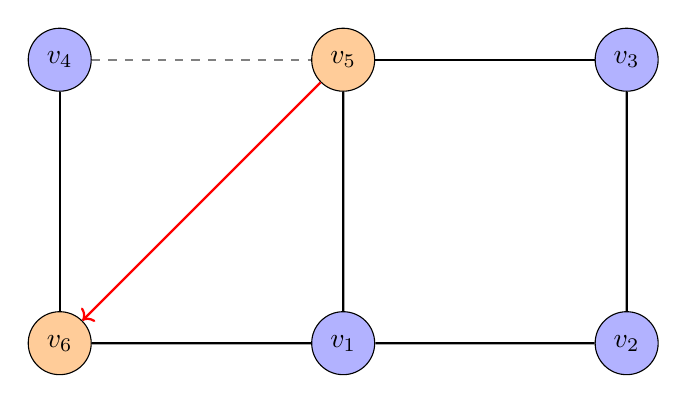
\begin{tikzpicture}[scale=1.8, 
    every node/.style={circle, draw, minimum size=0.8cm}]
    % Vertices - Step 2
    \node[fill=blue!30] (v4) at (0,0) {$v_4$};
    \node[fill=orange!40] (v5) at (2,0) {$v_5$};
    \node[fill=blue!30] (v3) at (4,0) {$v_3$};
    \node[fill=orange!40] (v6) at (0,-2) {$v_6$};
    \node[fill=blue!30] (v1) at (2,-2) {$v_1$};
    \node[fill=blue!30] (v2) at (4,-2) {$v_2$};
    
    % Edges
    \draw[thick, dashed, gray] (v4) -- (v5);
    \draw[thick] (v5) -- (v3);
    \draw[thick] (v4) -- (v6);
    \draw[thick] (v6) -- (v1);
    \draw[thick] (v1) -- (v2);
    \draw[thick] (v2) -- (v3);
    \draw[thick, red, ->] (v5) -- (v6);
    \draw[thick] (v1) -- (v5);
\end{tikzpicture}
\par}
{\centering
\small Figure 33: Step 2: Choose edge $\{v_5,v_6\}$. Vertices $v_5$ and $v_6$ are highlighted in orange. The previously traversed edge (from $v_4$ to $v_5$) is shown as a dashed gray line. A red directed arrow connects $v_5$ to $v_6$, showing the second edge chosen in the algorithm, following the rule of selecting edges that don't disconnect the graph.
\par}
\end{figure}

\begin{figure}[p]
{\centering
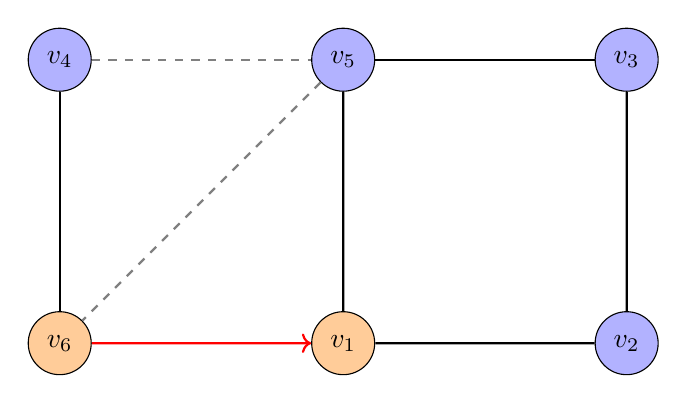
\begin{tikzpicture}[scale=1.8, 
    every node/.style={circle, draw, minimum size=0.8cm}]
    % Vertices - Step 3
    \node[fill=blue!30] (v4) at (0,0) {$v_4$};
    \node[fill=blue!30] (v5) at (2,0) {$v_5$};
    \node[fill=blue!30] (v3) at (4,0) {$v_3$};
    \node[fill=orange!40] (v6) at (0,-2) {$v_6$};
    \node[fill=orange!40] (v1) at (2,-2) {$v_1$};
    \node[fill=blue!30] (v2) at (4,-2) {$v_2$};
    
    % Edges
    \draw[thick, dashed, gray] (v4) -- (v5);
    \draw[thick] (v5) -- (v3);
    \draw[thick] (v4) -- (v6);
    \draw[thick, red, ->] (v6) -- (v1);
    \draw[thick] (v1) -- (v2);
    \draw[thick] (v2) -- (v3);
    \draw[thick, dashed, gray] (v5) -- (v6);
    \draw[thick] (v1) -- (v5);
\end{tikzpicture}
\par}
{\centering
\small Figure 34: Step 3: Choose edge $\{v_6,v_1\}$. Vertices $v_6$ and $v_1$ are highlighted in orange. Previously traversed edges ($v_4$-$v_5$ and $v_5$-$v_6$) are shown as dashed gray lines. A red directed arrow connects $v_6$ to $v_1$, representing the current edge being traversed in the Eulerian trail.
\par}
\end{figure}

\begin{figure}[p]
{\centering
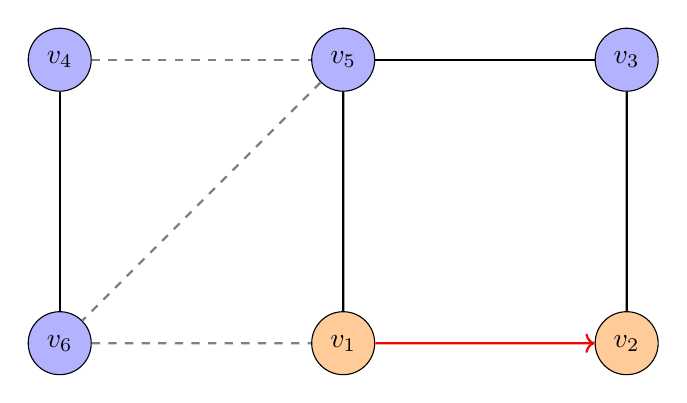
\begin{tikzpicture}[scale=1.8, 
    every node/.style={circle, draw, minimum size=0.8cm}]
    % Vertices - Step 4
    \node[fill=blue!30] (v4) at (0,0) {$v_4$};
    \node[fill=blue!30] (v5) at (2,0) {$v_5$};
    \node[fill=blue!30] (v3) at (4,0) {$v_3$};
    \node[fill=blue!30] (v6) at (0,-2) {$v_6$};
    \node[fill=orange!40] (v1) at (2,-2) {$v_1$};
    \node[fill=orange!40] (v2) at (4,-2) {$v_2$};
    
    % Edges
    \draw[thick, dashed, gray] (v4) -- (v5);
    \draw[thick] (v5) -- (v3);
    \draw[thick] (v4) -- (v6);
    \draw[thick, dashed, gray] (v6) -- (v1);
    \draw[thick, red, ->] (v1) -- (v2);
    \draw[thick] (v2) -- (v3);
    \draw[thick, dashed, gray] (v5) -- (v6);
    \draw[thick] (v1) -- (v5);
\end{tikzpicture}
\par}
{\centering
\small Figure 35: Step 4: Choose edge $\{v_1,v_2\}$. Vertices $v_1$ and $v_2$ are highlighted in orange. Three edges have now been traversed and appear as dashed gray lines. The current traversal from $v_1$ to $v_2$ is shown with a red directed arrow, continuing to follow the principle of choosing edges that maintain connectivity when possible.
\par}
\end{figure}

\begin{figure}[p]
{\centering
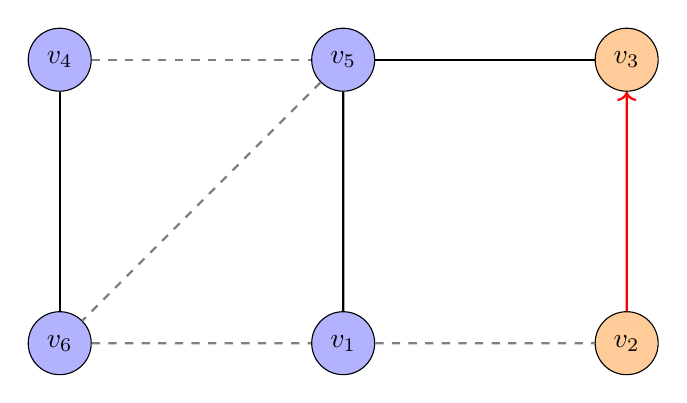
\begin{tikzpicture}[scale=1.8, 
    every node/.style={circle, draw, minimum size=0.8cm}]
    % Vertices - Step 5
    \node[fill=blue!30] (v4) at (0,0) {$v_4$};
    \node[fill=blue!30] (v5) at (2,0) {$v_5$};
    \node[fill=orange!40] (v3) at (4,0) {$v_3$};
    \node[fill=blue!30] (v6) at (0,-2) {$v_6$};
    \node[fill=blue!30] (v1) at (2,-2) {$v_1$};
    \node[fill=orange!40] (v2) at (4,-2) {$v_2$};
    
    % Edges
    \draw[thick, dashed, gray] (v4) -- (v5);
    \draw[thick] (v5) -- (v3);
    \draw[thick] (v4) -- (v6);
    \draw[thick, dashed, gray] (v6) -- (v1);
    \draw[thick, dashed, gray] (v1) -- (v2);
    \draw[thick, red, ->] (v2) -- (v3);
    \draw[thick, dashed, gray] (v5) -- (v6);
    \draw[thick] (v1) -- (v5);
\end{tikzpicture}
\par}
{\centering
\small Figure 36: Step 5: Choose edge $\{v_2,v_3\}$. Vertices $v_2$ and $v_3$ are highlighted in orange. Four previously traversed edges are shown as dashed gray lines. The current edge being traversed from $v_2$ to $v_3$ is indicated by a red directed arrow.
\par}
\end{figure}

\begin{figure}[p]
{\centering
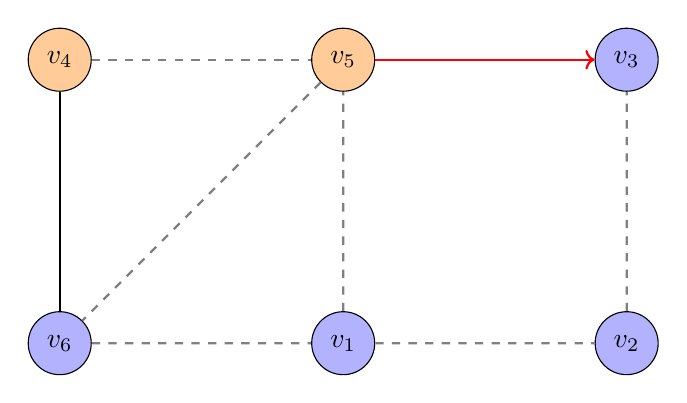
\begin{tikzpicture}[scale=1.8, 
    every node/.style={circle, draw, minimum size=0.8cm}]
    % Vertices - Step 6
    \node[fill=orange!40] (v4) at (0,0) {$v_4$};
    \node[fill=orange!40] (v5) at (2,0) {$v_5$};
    \node[fill=blue!30] (v3) at (4,0) {$v_3$};
    \node[fill=blue!30] (v6) at (0,-2) {$v_6$};
    \node[fill=blue!30] (v1) at (2,-2) {$v_1$};
    \node[fill=blue!30] (v2) at (4,-2) {$v_2$};
    
    % Edges
    \draw[thick, dashed, gray] (v4) -- (v5);
    \draw[thick, red, ->] (v5) -- (v3);
    \draw[thick] (v4) -- (v6);
    \draw[thick, dashed, gray] (v6) -- (v1);
    \draw[thick, dashed, gray] (v1) -- (v2);
    \draw[thick, dashed, gray] (v2) -- (v3);
    \draw[thick, dashed, gray] (v5) -- (v6);
    \draw[thick, dashed, gray] (v1) -- (v5);
\end{tikzpicture}
\par}
{\centering
\small Figure 37: Step 6: Choose edge $\{v_5,v_3\}$. Vertices $v_4$ and $v_5$ are highlighted in orange. Most edges have been traversed (shown as dashed gray lines). The current traversal is from $v_5$ to $v_3$, indicated by a red directed arrow. Note that the algorithm now traverses the remaining edges to complete the Eulerian trail.
\par}
\end{figure}

\begin{figure}[p]
{\centering
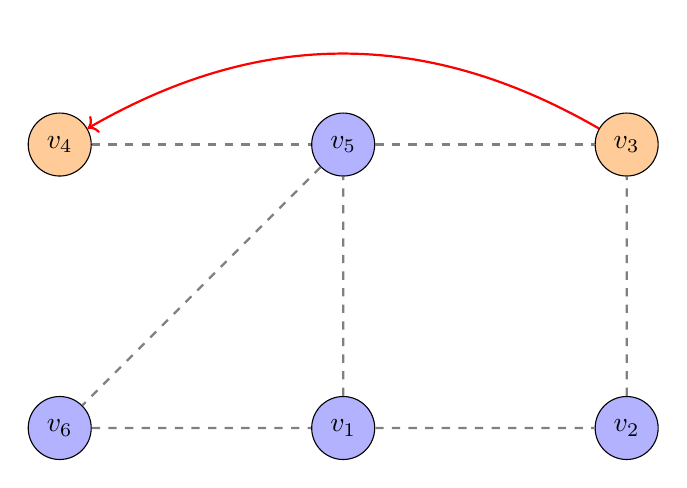
\begin{tikzpicture}[scale=1.8, 
    every node/.style={circle, draw, minimum size=0.8cm}]
    % Vertices - Step 7
    \node[fill=orange!40] (v4) at (0,0) {$v_4$};
    \node[fill=blue!30] (v5) at (2,0) {$v_5$};
    \node[fill=orange!40] (v3) at (4,0) {$v_3$};
    \node[fill=blue!30] (v6) at (0,-2) {$v_6$};
    \node[fill=blue!30] (v1) at (2,-2) {$v_1$};
    \node[fill=blue!30] (v2) at (4,-2) {$v_2$};
    
    % Edges
    \draw[thick, dashed, gray] (v4) -- (v5);
    \draw[thick, dashed, gray] (v5) -- (v3);
    \draw[thick, red, ->] (v3) to[bend right=30] (v4);
    \draw[thick, dashed, gray] (v6) -- (v1);
    \draw[thick, dashed, gray] (v1) -- (v2);
    \draw[thick, dashed, gray] (v2) -- (v3);
    \draw[thick, dashed, gray] (v5) -- (v6);
    \draw[thick, dashed, gray] (v1) -- (v5);
    
\end{tikzpicture}
\par}
{\centering
\small Figure 38: Step 7: Choose final edge $\{v_3,v_4\}$ to complete the tour. Vertices $v_4$ and $v_3$ are highlighted in orange with a red directed arrow from $v_3$ to $v_4$. This represents the completion of the Eulerian trail as the algorithm returns to the starting vertex after having traversed all edges in the graph exactly once.
\par}
\end{figure}

\begin{figure}[p]
{\centering
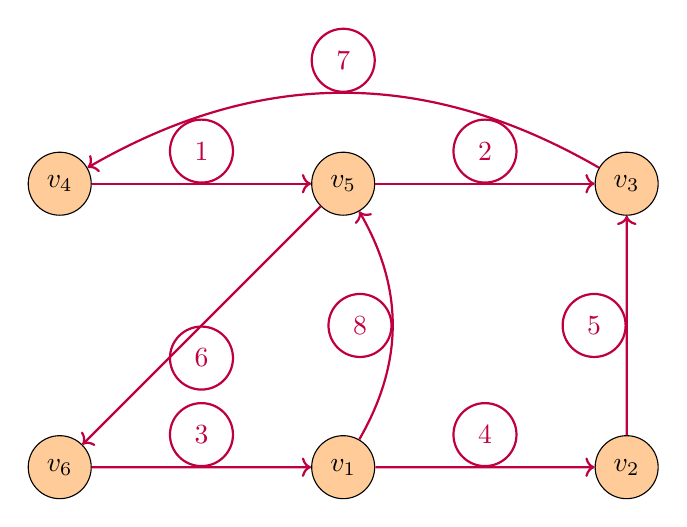
\begin{tikzpicture}[scale=1.8, 
    every node/.style={circle, draw, minimum size=0.8cm}]
    
    % Full tour
    \node[fill=orange!40] (v4) at (0,0) {$v_4$};
    \node[fill=orange!40] (v5) at (2,0) {$v_5$};
    \node[fill=orange!40] (v3) at (4,0) {$v_3$};
    \node[fill=orange!40] (v6) at (0,-2) {$v_6$};
    \node[fill=orange!40] (v1) at (2,-2) {$v_1$};
    \node[fill=orange!40] (v2) at (4,-2) {$v_2$};
    
    % Completed tour edges
    \draw[->, thick, purple] (v4) to node[above] {1} (v5);
    \draw[->, thick, purple] (v5) to node[below] {6} (v6);
    \draw[->, thick, purple] (v6) to node[above] {3} (v1);
    \draw[->, thick, purple] (v1) to node[above] {4} (v2);
    \draw[->, thick, purple] (v2) to node[left] {5} (v3);
    \draw[->, thick, purple] (v3) to[bend right=30] node[above] {7} (v4);
    \draw[->, thick, purple] (v5) to node[above] {2} (v3);
    \draw[->, thick, purple] (v1) to[bend right=30] node[left] {8} (v5);
\end{tikzpicture}
\par}
{\centering
\small Figure 39: Complete Eulerian tour using Fleury's Algorithm: $v_4 \rightarrow v_5 \rightarrow v_3 \rightarrow v_4 \rightarrow v_6 \rightarrow v_1 \rightarrow v_2 \rightarrow v_3$. All vertices are highlighted in orange, and all edges are shown as purple directed arrows with numbers indicating the order of traversal (1-8). This figure displays the entire Eulerian path found by the algorithm, showing how every edge in the graph is traversed exactly once.
\par}
\end{figure}

\begin{figure}[p]
{\centering
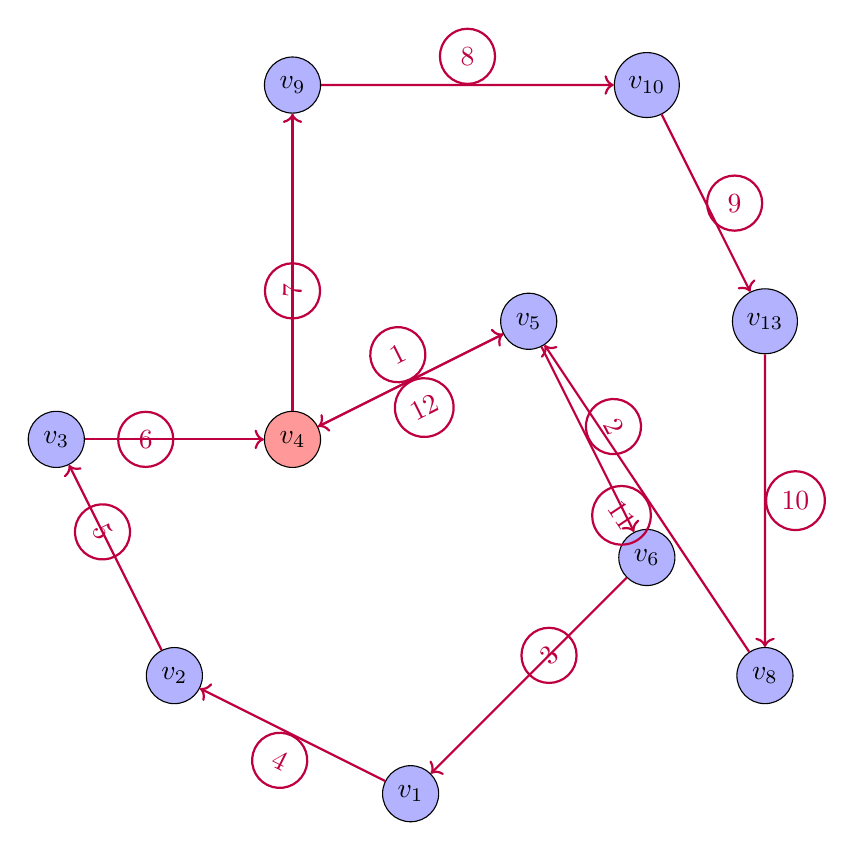
\begin{tikzpicture}[scale=1.5,
    every node/.style={circle, draw, minimum size=0.7cm}]
    % Vertices for the example
    \node[fill=red!40] (v4) at (0,0) {$v_4$};
    \node[fill=blue!30] (v5) at (2,1) {$v_5$};
    \node[fill=blue!30] (v6) at (3,-1) {$v_6$};
    \node[fill=blue!30] (v1) at (1,-3) {$v_1$};
    \node[fill=blue!30] (v2) at (-1,-2) {$v_2$};
    \node[fill=blue!30] (v3) at (-2,0) {$v_3$};
    \node[fill=blue!30] (v9) at (0,3) {$v_9$};
    \node[fill=blue!30] (v10) at (3,3) {$v_{10}$};
    \node[fill=blue!30] (v13) at (4,1) {$v_{13}$};
    \node[fill=blue!30] (v8) at (4,-2) {$v_8$};
    
    % Edges for the example
    \draw[->, thick, purple] (v4) to node[above, sloped] {1} (v5);
    \draw[->, thick, purple] (v5) to node[above, sloped] {2} (v6);
    \draw[->, thick, purple] (v6) to node[right, sloped] {3} (v1);
    \draw[->, thick, purple] (v1) to node[below, sloped] {4} (v2);
    \draw[->, thick, purple] (v2) to node[left, sloped] {5} (v3);
    \draw[->, thick, purple] (v3) to node[left, sloped] {6} (v4);
    \draw[->, thick, purple] (v4) to node[left, sloped] {7} (v9);
    \draw[->, thick, purple] (v9) to node[above] {8} (v10);
    \draw[->, thick, purple] (v10) to node[right] {9} (v13);
    \draw[->, thick, purple] (v13) to node[right] {10} (v8);
    \draw[->, thick, purple] (v8) to node[below, sloped] {11} (v5);
    \draw[->, thick, purple] (v5) to node[below, sloped] {12} (v4);
\end{tikzpicture}
\par}
{\centering
\small Figure 40: Example Eulerian tour: $v_4 \rightarrow v_5 \rightarrow v_6 \rightarrow v_1 \rightarrow v_2 \rightarrow v_3 \rightarrow v_4 \rightarrow v_9 \rightarrow v_{10} \rightarrow v_{13} \rightarrow v_8 \rightarrow v_5 \rightarrow v_4$. This figure shows a more complex example of an Eulerian tour on a larger graph with 10 vertices. The starting vertex $v_4$ is highlighted in red, and the complete tour is shown with purple directed arrows numbered 1-12. This demonstrates how Fleury's Algorithm scales to larger graphs while still finding a valid Eulerian path that traverses each edge exactly once before returning to the starting vertex.
\par}

\vspace{1em}
\begin{minipage}{\linewidth}
\begin{algorithm}[H]
\caption{Fleury's Algorithm for finding an Eulerian path or circuit}
\begin{algorithmic}[1]
\Procedure{Fleury}{$G(V,E)$, $start$}
    \State Let $currentVertex \gets start$
    \State Initialize empty list $path$
    \While{$E$ is not empty}
        \If{degree of $currentVertex$ is 1}
            \State Let $nextEdge$ be the only edge incident to $currentVertex$
        \Else
            \State Let $nextEdge$ be any edge incident to $currentVertex$ such that removing $nextEdge$ doesn't disconnect the graph
        \EndIf
        \State Let $nextVertex$ be the vertex at the other end of $nextEdge$
        \State Add $currentVertex$ to $path$
        \State Remove $nextEdge$ from $E$
        \State $currentVertex \gets nextVertex$
    \EndWhile
    \State Add $currentVertex$ to $path$ \Comment{Add the final vertex}
    \State \Return $path$
\EndProcedure
\end{algorithmic}
\end{algorithm}
\end{minipage}
\end{figure}

\pagebreak

\subsection{Eulerian Digraphs and DeBruijn Sequences}
\subsubsection{Eulerian Digraphs}

\begin{definition}[Eulerian Directed Graphs]
A directed graph (digraph) is Eulerian if there exists a closed walk that traverses each edge exactly once. The following properties characterize Eulerian digraphs:
\begin{enumerate}
    \item A digraph is Eulerian if and only if it is connected and the in-degree equals the out-degree for every vertex.
    \item A digraph has an Eulerian path (but not necessarily a cycle) if and only if:
    \begin{itemize}
        \item At most one vertex has $(\text{out-degree}) - (\text{in-degree}) = 1$
        \item At most one vertex has $(\text{in-degree}) - (\text{out-degree}) = 1$
        \item For all other vertices, in-degree equals out-degree
    \end{itemize}
\end{enumerate}
For a directed graph $G = (V, E)$, define:
\begin{align}
    d^+(v) &= \text{out-degree of vertex } v\\
    d^-(v) &= \text{in-degree of vertex } v
\end{align}
Then $G$ is Eulerian if and only if:
\begin{enumerate}
    \item $G$ is connected (or more precisely, the underlying undirected graph of $G$ is connected)
    \item $\forall v \in V, d^+(v) = d^-(v)$
\end{enumerate}
\end{definition}

\subsubsection{De Bruijn Sequences}


\begin{definition}[De Bruijn Sequence]
A De Bruijn sequence $B(k, n)$ is a cyclic sequence of length $k^n$ over an alphabet $A$ of size $k$ such that each possible string of length $n$ appears exactly once as a contiguous substring.
\end{definition}

\begin{properties}[De Bruijn Sequences]
\end{properties}
\vspace{0.5em} % Adds vertical space after the title

\begin{enumerate}
    \item The length of a De Bruijn sequence $B(k, n)$ is $k^n$.
    
    \item Every string of length $n$ over the alphabet appears exactly once as a substring.
    
    \item A De Bruijn sequence $B(k, n)$ can be viewed as a Hamiltonian path in the De Bruijn graph $G(k, n-1)$.
    
    \item The number of distinct De Bruijn sequences $B(k, n)$ is given by:
    \begin{equation}
        \frac{(k!)^{k^{n-1}}}{k^n}
    \end{equation}
    
    \item More specifically, the number of binary De Bruijn sequences $B(2, n)$ is:
    \begin{equation}
        2^{2^{n-1}-n}
    \end{equation}
\end{enumerate}

\begin{properties}[Connection to Eulerian Digraphs]
De Bruijn sequences have a fundamental connection to Eulerian digraphs:
\begin{enumerate}
    \item A De Bruijn graph $G(k, n-1)$ is a directed graph with $k^{n-1}$ vertices, each labeled with a string of length $n-1$.
    \item There is an edge from vertex $u$ to vertex $v$ if the last $n-2$ symbols of $u$ match the first $n-2$ symbols of $v$.
    \item For every vertex in $G(k, n-1)$, the in-degree equals the out-degree (both equal to $k$).
    \item Therefore, $G(k, n-1)$ is an Eulerian digraph.
    \item A De Bruijn sequence $B(k, n)$ corresponds to an Eulerian circuit in $G(k, n-1)$.
\end{enumerate}
\end{properties}

\begin{properties}[Mathematical Structure]
The adjacency matrix $A$ of the De Bruijn graph $G(k, n)$ has the following properties:
\begin{enumerate}
    \item $A$ is a $k^n \times k^n$ matrix.
    \item $A_{i,j} = 1$ if the last $n-1$ symbols of vertex $i$ match the first $n-1$ symbols of vertex $j$.
    \item $A_{i,j} = 0$ otherwise.
    \item The number of Eulerian circuits (and thus De Bruijn sequences) can be computed using the BEST theorem:
    \begin{equation}
        \text{Number of Eulerian circuits} = t_w \prod_{v \in V} (d^+(v) - 1)!
    \end{equation}
    where $t_w$ is the number of oriented spanning trees rooted at vertex $w$.
\end{enumerate}
\end{properties}

\begin{properties}[Combinatorial Aspects] The combinatorial aspects of De Bruijn Sequence B(k,n) has the following properties
\begin{enumerate}
    \item A De Bruijn sequence can be constructed from a Eulerian circuit in the De Bruijn graph $G(k, n-1)$.
    \item Every De Bruijn sequence $B(k, n)$ contains $k^n$ distinct substrings of length $n$.
    \item The De Bruijn sequence has a feedback function $f$ that generates the next bit:
    \begin{equation}
        a_{i+n} = f(a_i, a_{i+1}, \ldots, a_{i+n-1})
    \end{equation}
\end{enumerate}
\end{properties}
\begin{theorem}[Generating Function]
For a binary De Bruijn sequence, the generating function can be expressed as:
\begin{equation}
    G(x) = \sum_{i=0}^{2^n-1} a_i x^i \mod (x^{2^n} - 1)
\end{equation}
where $a_i$ represents the $i$-th element in the sequence.
\end{theorem}

\begin{theorem}[LFSR Representation]
A binary De Bruijn sequence can be generated using a Linear Feedback Shift Register with the characteristic polynomial:
\begin{equation}
    p(x) = x^n + c_{n-1}x^{n-1} + \cdots + c_1x + c_0
\end{equation}
The recurrence relation is:
\begin{equation}
    a_{i+n} = c_0a_i \oplus c_1a_{i+1} \oplus \cdots \oplus c_{n-1}a_{i+n-1}
\end{equation}
where $\oplus$ represents the XOR operation.
\end{theorem}

\begin{theorem}[Counting Formula]
The number of distinct De Bruijn sequences $B(k, n)$ is:
\begin{equation}
    N(k, n) = \frac{k!^{k^{n-1}}}{k^n}
\end{equation}

For the binary case $B(2, n)$, the number of distinct sequences is:
\begin{equation}
    N(2, n) = 2^{2^{n-1}-n}
\end{equation}
\end{theorem}

\begin{example}[Small Values]
The number of distinct De Bruijn sequences for small parameters:
\begin{align}
    N(2, 2) &= 1 \\
    N(2, 3) &= 2 \\
    N(2, 4) &= 16 \\
    N(2, 5) &= 2048 \\
    N(3, 2) &= 2 \\
    N(3, 3) &= 48 \\
    N(4, 2) &= 24
\end{align}
\end{example}
\begin{theorem}[FKM Algorithm]
The FKM (Fredricksen, Kessler, Maiorana) algorithm constructs a binary De Bruijn sequence $B(2, n)$ by generating all necklaces of length $n$, ordering them lexicographically, replacing each with its aperiodic prefixes, and concatenating the last bits of these prefixes in order.
\end{theorem}

\begin{algorithm}
\caption{FKM Algorithm for $B(2, n)$}
\begin{algorithmic}[1]
\Require Integer $n \geq 2$
\Ensure Binary De Bruijn sequence $B(2, n)$
\State $S \gets \text{empty sequence}$
\Function{GenerateNecklaces}{$n$}
    \State $N \gets \emptyset$; $\text{seen} \gets \emptyset$
    \For{all binary strings $b$ of length $n$ in lexicographic order}
        \If{$b \notin \text{seen}$}
            \State $\text{necklace} \gets \text{smallest rotation of } b$
            \State $N \gets N \cup \{\text{necklace}\}$; $\text{seen} \gets \text{seen} \cup \{\text{all rotations of } b\}$
        \EndIf
    \EndFor
    \State \Return $N$
\EndFunction
\Function{GetAperiodicPrefixes}{necklace}
    \State $prefixes \gets \emptyset$; $p \gets \text{period of necklace}$
    \For{$i \gets 1$ to $p$}
        \State $prefixes \gets prefixes \cup \{\text{first } i \text{ bits of necklace}\}$
    \EndFor
    \State \Return $prefixes$
\EndFunction
\State $necklaces \gets \text{Sort}(\text{GenerateNecklaces}(n))$
\For{each $necklace$ in $necklaces$}
    \For{each $prefix$ in $\text{GetAperiodicPrefixes}(necklace)$}
        \State $S \gets S \cdot \text{last bit of } prefix$
    \EndFor
\EndFor
\State \Return $S$
\end{algorithmic}
\end{algorithm}

\begin{remark}
The FKM algorithm can also be implemented using Lyndon words:
\end{remark}

\begin{algorithm}
\caption{Lyndon-based FKM Algorithm}
\begin{algorithmic}[1]
\Require Integer $n \geq 2$
\Ensure Binary De Bruijn sequence $B(2, n)$
\Function{IsLyndonWord}{$w$}
    \For{$i \gets 1$ to $|w|-1$}
        \If{$w =$ rotation of $w$ by $i$ or $w >$ rotation of $w$ by $i$}
            \State \Return false
        \EndIf
    \EndFor
    \State \Return true
\EndFunction
\Function{Period}{$w$}
    \For{$i \gets 1$ to $|w|$}
        \If{$w =$ rotation of $w$ by $i$} \Return $i$ \EndIf
    \EndFor
    \State \Return $|w|$
\EndFunction
\State $S \gets \text{empty sequence}$
\For{each binary string $w$ of length $n$ in lexicographic order}
    \If{IsLyndonWord($w$)}
        \State $period \gets \text{Period}(w)$
        \For{$i \gets 1$ to $period$}
            \State $S \gets S \cdot \text{last bit of first } i \text{ bits of } w$
        \EndFor
    \EndIf
\EndFor
\State \Return $S$
\end{algorithmic}
\end{algorithm}

\begin{theorem}[Prefer-1 Algorithm]
The Prefer-1 algorithm generates a binary De Bruijn sequence $B(2, n)$ by starting with $n$ zeros and repeatedly appending either a 1 (preferred) or a 0, choosing whichever creates a new $n$-tuple that hasn't appeared before in the sequence.
\end{theorem}

\begin{algorithm}
\caption{Prefer-1 Algorithm for $B(2, n)$}
\begin{algorithmic}[1]
\Require Integer $n \geq 2$
\Ensure Binary De Bruijn sequence $B(2, n)$
\State $R \gets $ n-bit register initialized to all zeros
\State $S \gets $ sequence of $n$ zeros \Comment{Output the initial $n$ zeros}
\State $seen \gets \{R\}$ \Comment{Set of seen $n$-tuples, initially contains all zeros}

\While{$|seen| < 2^n$}
    \State $R_{next1} \gets $ last $n-1$ bits of $R$ followed by 1
    \If{$R_{next1} \notin seen$}
        \State $R \gets R_{next1}$ \Comment{Shift in a 1}
        \State $S \gets S \cdot 1$ \Comment{Append 1 to output}
    \Else
        \State $R \gets $ last $n-1$ bits of $R$ followed by 0 \Comment{Shift in a 0}
        \State $S \gets S \cdot 0$ \Comment{Append 0 to output}
    \EndIf
    \State $seen \gets seen \cup \{R\}$
\EndWhile
\State \Return $S$
\end{algorithmic}
\end{algorithm}

\begin{theorem}[Correctness]
The Prefer-1 algorithm correctly generates a binary De Bruijn sequence of order $n$ with length $2^n$.
\end{theorem}

\begin{remark}
The Prefer-1 algorithm can be viewed as a greedy approach that traverses a De Bruijn graph by always choosing the edge labeled 1 when possible. It represents a special case of the more general Prefer-$d$ algorithm for arbitrary alphabet sizes.
\end{remark}

\begin{theorem}[Prefer-Opposite Algorithm]
The Prefer-Opposite algorithm generates a binary De Bruijn sequence $B(2, n)$ by starting with $n$ zeros and repeatedly appending the opposite of the last bit (when possible) or the same as the last bit, choosing whichever creates a new $n$-tuple that hasn't appeared before in the sequence.
\end{theorem}

\begin{algorithm}
\caption{Prefer-Opposite Algorithm for $B(2, n)$}
\begin{algorithmic}[1]
\Require Integer $n \geq 2$
\Ensure Binary De Bruijn sequence $B(2, n)$
\State $R \gets $ n-bit register initialized to all zeros
\State $S \gets $ sequence of $n$ zeros \Comment{Output the initial $n$ zeros}
\State $last \gets 0$ \Comment{Last bit output}
\State $seen \gets \{R\}$ \Comment{Set of seen $n$-tuples, initially contains all zeros}

\While{$|seen| < 2^n$}
    \State $opposite \gets 1-last$ \Comment{Opposite of the last bit}
    \State $R_{next} \gets $ last $n-1$ bits of $R$ followed by $opposite$
    \If{$R_{next} \notin seen$}
        \State $last \gets opposite$ \Comment{Prefer the opposite}
    \Else
        \State $R_{next} \gets $ last $n-1$ bits of $R$ followed by $last$
    \EndIf
    \State $R \gets R_{next}$ \Comment{Update register}
    \State $S \gets S \cdot last$ \Comment{Append bit to output}
    \State $seen \gets seen \cup \{R\}$
\EndWhile
\State \Return $S$
\end{algorithmic}
\end{algorithm}

\begin{theorem}[Correctness]
The Prefer-Opposite algorithm correctly generates a binary De Bruijn sequence of order $n$ with length $2^n$.
\end{theorem}

\begin{remark}
The Prefer-Opposite algorithm creates sequences with different balance properties than the Prefer-1 algorithm, often resulting in a more even distribution of 0s and 1s. This approach can be generalized to larger alphabets by defining a suitable notion of "opposite."
\end{remark}
\begin{theorem}[Huang's Cycle-Joining Algorithm]
Huang's algorithm constructs a De Bruijn sequence $B(k, n)$ by first generating all disjoint cycles of a feedback shift register, then identifying a spanning tree of the cycle graph, and systematically joining cycles according to the spanning tree to form a single cycle containing all states.
\end{theorem}

\begin{algorithm}
\caption{Huang's Cycle-Joining Algorithm for $B(k, n)$}
\begin{algorithmic}[1]
\Require Integer $n \geq 2$, alphabet size $k \geq 2$
\Ensure De Bruijn sequence $B(k, n)$
\Function{GenerateFSRCycles}{$n, k$}
    \State Generate all disjoint cycles formed by the feedback shift register
    \State \Return set of all cycles $C = \{C_1, C_2, \ldots, C_m\}$
\EndFunction

\Function{BuildCycleGraph}{$C$}
    \State $G \gets$ empty graph with vertices representing cycles
    \For{each cycle $C_i$ in $C$}
        \State Add a vertex $v_i$ to $G$ representing cycle $C_i$
    \EndFor
    \For{each pair of cycles $C_i, C_j$ with a potential joining state}
        \State Add an edge $(v_i, v_j)$ to $G$ labeled with the joining state
    \EndFor
    \State \Return $G$
\EndFunction

\Function{JoinCycles}{$C_i, C_j, s$}
    \State $s$ is a state appearing in both cycles at different predecessors
    \State Redirect transitions to merge $C_i$ and $C_j$ into a single cycle
    \State \Return the merged cycle
\EndFunction

\State $cycles \gets \text{GenerateFSRCycles}(n, k)$
\State $G \gets \text{BuildCycleGraph}(cycles)$

\State $connectedCycles \gets \emptyset$ \Comment{Set of cycles already joined}
\State $joinEdges \gets \emptyset$ \Comment{Set of edges used to join cycles}
\State $result \gets$ first cycle in $cycles$
\State $connectedCycles \gets connectedCycles \cup \{result\}$

\While{$|connectedCycles| < |cycles|$}
    \State $bestEdge \gets \text{null}$
    \For{each edge $(v_i, v_j)$ in $G$ where $v_i$ represents a cycle in $connectedCycles$ and $v_j$ doesn't}
        \If{$bestEdge$ is $\text{null}$ or edge $(v_i, v_j)$ is preferred for joining}
            \State $bestEdge \gets (v_i, v_j)$
        \EndIf
    \EndFor
    
    \State Add cycle represented by $v_j$ to $connectedCycles$
    \State $joinEdges \gets joinEdges \cup \{bestEdge\}$
    \State $s \gets$ joining state associated with $bestEdge$
    \State $result \gets \text{JoinCycles}(result, \text{cycle for } v_j, s)$
\EndWhile

\State \Return sequence representation of $result$
\end{algorithmic}
\end{algorithm}

\begin{theorem}[Correctness]
Huang's Cycle-Joining algorithm correctly generates a De Bruijn sequence of order $n$ over an alphabet of size $k$ with length $k^n$.
\end{theorem}

\begin{remark}
Huang's algorithm provides a general approach that works for any alphabet size and offers flexibility in how cycles are joined, enabling the construction of De Bruijn sequences with specific properties by choosing different spanning trees of the cycle graph.
\end{remark}


\begin{remark}[Non-uniqueness]
De Bruijn sequences are not unique for $n > 2$. The number of distinct De Bruijn sequences $B(2,n)$ is given by $2^{2^{n-1}-n}$, which grows rapidly with $n$. For example, there are 2 distinct $B(2,3)$ sequences and 16 distinct $B(2,4)$ sequences.
\end{remark}

\subsection{De Bruijn Graphs}
\begin{definition}[De Bruijn Graph]
A De Bruijn graph $G(k,n)$ is a directed graph representing all possible sequences of a given length over a given alphabet:

\begin{enumerate}
    \item The graph has $k^{n-1}$ vertices, where $k$ is the alphabet size.
    \item Each vertex represents a sequence of length $n-1$ over the alphabet.
    \item There is a directed edge from vertex $u$ to vertex $v$ if the last $n-2$ symbols of $u$ match the first $n-2$ symbols of $v$.
    \item Each edge is labeled with the symbol that extends the sequence represented by $u$ to obtain the sequence for the destination vertex $v$.
    \item The graph has exactly $k^n$ edges.
    \item For every vertex, the in-degree equals the out-degree (both equal to $k$).
    \item A De Bruijn sequence $B(k,n)$ corresponds to an Eulerian cycle in this graph.
\end{enumerate}
\end{definition}

\begin{figure}[ht]
  \centering
  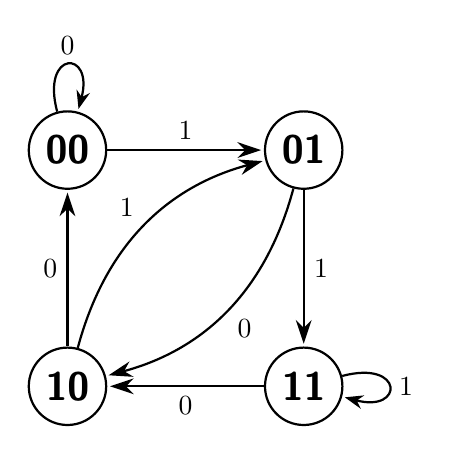
\begin{tikzpicture}[
      > = Stealth,
      shorten > = 1pt,
      auto,
      node distance = 3cm,
      thick,
      main node/.style = {circle, draw, font=\sffamily\Large\bfseries}
  ]
  % Define the vertices (nodes)
  \node[main node] (00) at (0,3) {00};
  \node[main node] (01) at (3,3) {01};
  \node[main node] (10) at (0,0) {10};
  \node[main node] (11) at (3,0) {11};

  % Define the edges with labels
  % From 00
  \path[->] (00) edge[loop above] node {0} (00);
  \path[->] (00) edge node {1} (01);

  % From 01
  \path[->] (01) edge[bend left] node {0} (10);
  \path[->] (01) edge node {1} (11);

  % From 10
  \path[->] (10) edge node {0} (00);
  \path[->] (10) edge[bend left] node {1} (01);

  % From 11
  \path[->] (11) edge node {0} (10);
  \path[->] (11) edge[loop right] node {1} (11);
  \end{tikzpicture}

  {\centering
\small Figure 41:De Bruijn Graph $B(2,3)$. This directed graph has 4 vertices representing all 2-bit sequences, and 8 edges labeled by the appended bit. An Eulerian circuit on this graph yields a de Bruijn sequence of order~3 over a binary alphabet. \par}
\end{figure}

\begin{figure}[ht]
{\centering
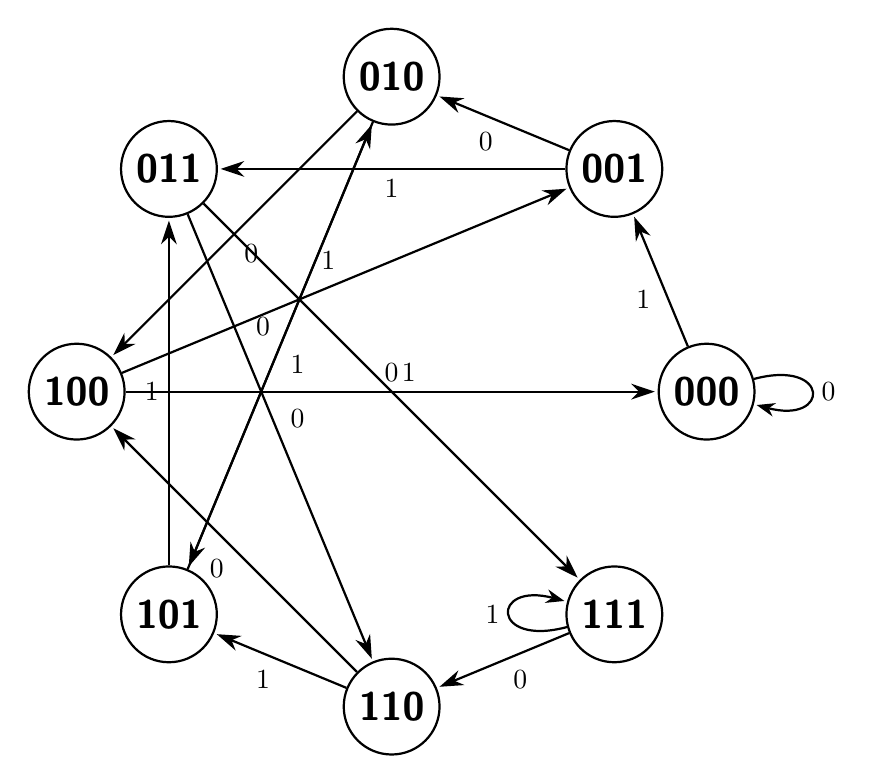
\begin{tikzpicture}[
    > = Stealth,
    shorten > = 1pt,
    auto,
    thick,
    main node/.style = {circle, draw, font=\sffamily\Large\bfseries}
]
% Define vertices in an octagonal arrangement
\def\radius{4}
\node[main node] (000) at ({\radius*cos(0)},{\radius*sin(0)}) {000};
\node[main node] (001) at ({\radius*cos(45)},{\radius*sin(45)}) {001};
\node[main node] (010) at ({\radius*cos(90)},{\radius*sin(90)}) {010};
\node[main node] (011) at ({\radius*cos(135)},{\radius*sin(135)}) {011};
\node[main node] (100) at ({\radius*cos(180)},{\radius*sin(180)}) {100};
\node[main node] (101) at ({\radius*cos(225)},{\radius*sin(225)}) {101};
\node[main node] (110) at ({\radius*cos(270)},{\radius*sin(270)}) {110};
\node[main node] (111) at ({\radius*cos(315)},{\radius*sin(315)}) {111};

% Define the edges with labels
% From 000
\path[->] (000) edge[loop right] node {0} (000);
\path[->] (000) edge node {1} (001);

% From 001
\path[->] (001) edge node {0} (010);
\path[->] (001) edge node {1} (011);

% From 010
\path[->] (010) edge node {0} (100);
\path[->] (010) edge node {1} (101);

% From 011
\path[->] (011) edge node {0} (110);
\path[->] (011) edge node {1} (111);

% From 100
\path[->] (100) edge node {0} (000);
\path[->] (100) edge node {1} (001);

% From 101
\path[->] (101) edge node {0} (010);
\path[->] (101) edge node {1} (011);

% From 110
\path[->] (110) edge node {0} (100);
\path[->] (110) edge node {1} (101);

% From 111
\path[->] (111) edge node {0} (110);
\path[->] (111) edge[loop left] node {1} (111);

\end{tikzpicture}
\par}
{\centering
\small Figure 42: De Bruijn Graph $B(2,4)$. This directed graph has 8 vertices representing all possible 3-bit binary sequences (000 through 111). Each edge is labeled with the bit (0 or 1) that is appended when transitioning between states. The graph has 16 edges in total, and a De Bruijn sequence $B(2,4)$ corresponds to an Eulerian circuit traversing all edges exactly once.
\par}
\end{figure}
\begin{lemma}[Connection to Eulerian Circuits]
A De Bruijn sequence $B(k,n)$ corresponds exactly to an Eulerian circuit in the De Bruijn graph $B(k,n-1)$.
\end{lemma}
\begin{proof}[Proof sketch]
Each edge in the De Bruijn graph $B(k,n-1)$ represents the transition from one $(n-1)$-length sequence to another by appending a symbol and removing the first symbol. Following an Eulerian circuit through all edges generates each possible $n$-length sequence exactly once, which is precisely the definition of a De Bruijn sequence.
\end{proof}
\begin{lemma}[Fundamental Property of De Bruijn Graphs]
For any alphabet size $k$ and order $n$, the De Bruijn graph $B(k,n)$ has exactly $k^n$ vertices and $k^{n+1}$ edges.
\end{lemma}
\begin{proof}
Each vertex in $B(k,n)$ represents a sequence of $n$ symbols from an alphabet of size $k$, giving exactly $k^n$ possible vertices. From each vertex, there are $k$ possible transitions (one for each symbol in the alphabet), resulting in exactly $k \cdot k^n = k^{n+1}$ edges.
\end{proof}
\begin{lemma}[Connection to Eulerian Circuits]
A De Bruijn sequence $B(k,n)$ corresponds exactly to an Eulerian circuit in the De Bruijn graph $B(k,n-1)$.
\end{lemma}
\begin{proof}[Proof sketch]
Each edge in the De Bruijn graph $B(k,n-1)$ represents the transition from one $(n-1)$-length sequence to another by appending a symbol and removing the first symbol. Following an Eulerian circuit through all edges generates each possible $n$-length sequence exactly once, which is precisely the definition of a De Bruijn sequence.
\end{proof}
\begin{remark}[Relationship to Universal Cycles]
De Bruijn sequences are a special case of universal cycles, which are cyclic sequences where each object from a set appears exactly once as a consecutive substring. When the objects are all possible $n$-tuples from a $k$-symbol alphabet, the universal cycle is precisely a De Bruijn sequence of order $n$.
\end{remark}
\begin{theorem}[Line Graph Relationship]
The De Bruijn graph $B(k,n+1)$ is isomorphic to the line graph of $B(k,n)$.
\end{theorem}

\begin{proof}
In the line graph of $B(k,n)$, each vertex corresponds to an edge in $B(k,n)$. An edge in $B(k,n)$ represents a transition from an $n$-length sequence to another by appending a symbol and removing the first symbol, which results in an $(n+1)$-length sequence. This exactly corresponds to a vertex in $B(k,n+1)$. Two vertices in the line graph are adjacent if their corresponding edges in $B(k,n)$ form a directed path of length 2, which precisely matches the adjacency condition in $B(k,n+1)$.
\end{proof}
\begin{theorem}[Shift Register Implementation]
Every binary De Bruijn sequence of order $n$ can be generated by a linear feedback shift register of length $n$ with an appropriate feedback function.
\end{theorem}

\begin{proof}[Proof outline]
Consider an $n$-bit shift register with bits $(b_1, b_2, \ldots, b_n)$. For each state of the register, we compute the next bit $b_{n+1}$ using a feedback function $f(b_1, b_2, \ldots, b_n)$. This bit is then shifted into the register, and $b_1$ is discarded.

For a De Bruijn sequence, we need a feedback function $f$ such that the shift register cycles through all $2^n$ possible states before repeating. This can be achieved by defining $f$ such that:

1. For the state $(0, 0, \ldots, 0)$, $f$ outputs 1 (to avoid the cycle containing only zeros)
2. For all other states, $f$ is chosen strategically to ensure a maximal cycle

One such function for binary De Bruijn sequences is:
\begin{center}
$f(b_1, b_2, \ldots, b_n) = b_1 \oplus b_2 \oplus \cdots \oplus b_{n-1} \oplus (b_n \lor 1)$
\end{center}
where $\oplus$ is XOR and $\lor$ is OR. This produces a modified maximum-length sequence that includes all $2^n$ possible states.
\end{proof}
\pagebreak
\pagebreak
\clearpage
\subsection{Chapter 2 Exercises}
\subsubsection{Easy Problems: Eulerian Graphs}
\begin{enumerate}
    \item Determine whether the following graph is Eulerian, semi-Eulerian, or neither:
    A graph with vertices $\{A, B, C, D, E\}$ and edges $\{(A,B), (B,C), (C,D), (D,E), (E,A), (A,C), (C,E)\}$
    
    \item Prove that a connected graph has an Eulerian path if and only if it has exactly 0 or 2 vertices with odd degree.
    
    \item Construct a simple graph with 6 vertices that has an Eulerian circuit. How many edges must such a graph have at minimum?
    
    \item Given a connected graph where all vertices have even degree, prove that it has an Eulerian circuit.

    
\end{enumerate}

\subsubsection{Medium Problems: Eulerian Graphs}
\begin{enumerate}[resume]
    \item A village has 7 bridges connecting different areas. Is it possible to walk through the village crossing each bridge exactly once? If so, find such a path. If not, explain why.
    
    \item Show that if $G$ is a connected graph where every vertex has even degree, then removing any edge results in a graph that has an Eulerian path but not an Eulerian circuit.
    
    \item Given a connected graph $G$ with $2k$ vertices of odd degree ($k \geq 1$), what is the minimum number of paths needed to cover all edges of $G$ exactly once?
    
    \item Prove that if $G$ is a connected graph with exactly two vertices of odd degree, say $u$ and $v$, then there exists an Eulerian path from $u$ to $v$.
\end{enumerate}

\subsubsection{Hard Problems: Eulerian Graphs}
\begin{enumerate}[resume]
    \item Prove that a connected graph $G$ has an Eulerian circuit if and only if its edge set can be partitioned into simple cycles.
    
    \item Consider a complete graph $K_n$. For which values of $n$ does $K_n$ have an Eulerian circuit? Provide a proof for your answer.
    
    \item Let $G$ be a connected graph with an even number of edges. Prove that the edges of $G$ can be partitioned into paths of length 2 if and only if $G$ has no vertices of odd degree.
    
    \item For a connected graph $G$, let $o(G)$ denote the number of vertices with odd degree. If $G_1, G_2, \ldots, G_k$ are the connected components of $G$, prove that $\sum_{i=1}^{k} o(G_i)$ is even.
\end{enumerate}

\subsubsection{Easy Problems: De Bruijn Sequences}
\begin{enumerate}[resume]
    \item Construct a binary De Bruijn sequence of order 3 (i.e., a circular sequence where every possible 3-length binary string appears exactly once as a substring).
    
    \item How many distinct binary De Bruijn sequences of order 4 exist? Explain your reasoning.
    
    \item For a ternary alphabet $\{0,1,2\}$, what is the length of a De Bruijn sequence of order 2? List all possible substrings that must appear exactly once.
    
    
\end{enumerate}

\subsubsection{Medium Problems: De Bruijn Sequences}
\begin{enumerate}[resume]
    \item Prove that for any alphabet of size $k$, a De Bruijn sequence of order $n$ has length $k^n$.
    
    \item Construct a De Bruijn sequence of order 2 for an alphabet of size 3. Then describe an algorithm to generate such sequences for any alphabet size.
    
    \item Show how to construct a De Bruijn sequence of order $n+1$ from a De Bruijn sequence of order $n$.
    
    \item Given a binary De Bruijn sequence of order 4, describe how many different such sequences exist and explain an algorithm to generate them.
\end{enumerate}

\subsubsection{Hard Problems: De Bruijn Sequences}
\begin{enumerate}[resume]
    \item Prove that any De Bruijn sequence of order $n$ for an alphabet of size $k$ can be represented as an Eulerian circuit in a directed graph with $k^{n-1}$ vertices.
    
    \item Given a De Bruijn sequence of order $n$ over alphabet $\{0,1\}$, describe an algorithm to find the position of any $n$-length binary string within the sequence without examining the entire sequence.
    
    \item Prove that for any binary De Bruijn sequence of order $n$, there exists a corresponding binary necklace of length $2^n - 1$.
\end{enumerate}

\subsubsection{Easy Problems: De Bruijn Graphs}
\begin{enumerate}[resume]
    \item Draw the De Bruijn Graph of order 1 for the binary alphabet $\{0,1\}$. How many vertices and edges does it have?
    
    \item For a ternary alphabet $\{0,1,2\}$, construct the De Bruijn Graph of order 1. How many vertices and edges does it have?
    \item Draw the De Bruijn Graph of order 2 for the binary alphabet $\{0,1\}$. Then trace a path through this diagram that generates a De Bruijn sequence of order 3.
    
    \item Draw a binary De Bruijn Graph of order 1 (with vertices $0$ and $1$). Then draw the corresponding De Bruijn Graph of order 2 using the line graph construction.
    
    \item Draw a De Bruijn Graph for a ternary alphabet $\{0,1,2\}$ of order 1. Find an Eulerian circuit in this diagram and write down the corresponding De Bruijn sequence.
\end{enumerate}

\subsubsection{Medium Problems: De Bruijn Graphs}
\begin{enumerate}[resume]
    \item Prove that the De Bruijn Graph $B(k,n)$ has $k^n$ vertices and $k^{n+1}$ edges.
    
    \item Consider a modified De Bruijn graph where certain transitions are forbidden. Specifically, in a binary De Bruijn graph of order 3, transitions to states containing "$111$" are prohibited. Is it still possible to find an Eulerian path in this modified diagram? If so, construct one. If not, explain why.
\end{enumerate}

\subsubsection{Hard Problems: De Bruijn Graphs}
\begin{enumerate}[resume]
    \item Let $B(k,n)$ be the De Bruijn graph of order $n$ over an alphabet of size $k$. Prove that the line graph of $B(k,n)$ is isomorphic to $B(k,n+1)$.
    
    \item For a De Bruijn Graph $B(2,n)$, determine the chromatic number of the underlying undirected graph and prove your answer.
\end{enumerate}

\clearpage

\section{Hamiltonian Graphs}
\subsection{Hamiltonian Walks, Paths, Cycles}

\begin{definition}[Hamiltonian Cycle]
A Hamiltonian cycle in a graph $G$ is a cycle that visits each vertex of $G$ exactly once (except for the starting vertex, which is also the ending vertex). Equivalently, a Hamiltonian cycle is a spanning cycle of the graph, meaning $V(C) = V(G)$. A graph is called Hamiltonian if it contains a Hamiltonian cycle.
\end{definition}

\begin{definition}[Hamiltonian Path]
A Hamiltonian path in a graph $G$ is a path that visits each vertex of $G$ exactly once. Equivalently, a Hamiltonian path is a spanning path in the graph, meaning $V(P) = V(G)$. A graph is called traceable if it contains a Hamiltonian path.
\end{definition}

\begin{figure}[H]
    \centering
    \begin{tikzpicture}[
        vertex/.style={circle, draw=black, thick, fill=blue!15, minimum size=0.8cm, font=\bfseries},
        normaledge/.style={draw, thick, black!30},
        pathedge/.style={draw, very thick, red!80!black, -latex}
    ]
        % Vertices
        \node[vertex] (A) at (0,3) {$A$};
        \node[vertex] (B) at (2,4) {$B$};
        \node[vertex] (C) at (4,3) {$C$};
        \node[vertex] (D) at (3,1) {$D$};
        \node[vertex] (E) at (1,1) {$E$};
        
        % All edges (grayed out)
        \draw[normaledge] (A) -- (B);
        \draw[normaledge] (B) -- (C);
        \draw[normaledge] (C) -- (D);
        \draw[normaledge] (D) -- (E);
        \draw[normaledge] (E) -- (A);
        \draw[normaledge] (A) -- (C);
        \draw[normaledge] (B) -- (D);
        
        % Hamiltonian path (highlighted)
        \draw[pathedge] (A) -- (B);
        \draw[pathedge] (B) -- (C);
        \draw[pathedge] (C) -- (D);
        \draw[pathedge] (D) -- (E);
        
        % Label
        \node[align=center, font=\sffamily\bfseries] at (2,0) {Hamiltonian Path: $A \to B \to C \to D \to E$};
    \end{tikzpicture}
    
    \vspace{0.2cm}
    \begin{center}
    \small Figure 43: Example of a Hamiltonian path. The red path visits every vertex of the graph exactly once, making it a Hamiltonian path. Unlike Eulerian paths which must traverse every edge exactly once, a Hamiltonian path must visit every vertex exactly once.
    \end{center}
\end{figure}

\begin{figure}[H]
    \centering
    \begin{tikzpicture}[
        vertex/.style={circle, draw=black, thick, fill=blue!15, minimum size=0.8cm, font=\bfseries},
        normaledge/.style={draw, thick, black!30},
        cycleedge/.style={draw, very thick, red!80!black, -latex}
    ]
        % Vertices
        \node[vertex] (A) at (0,3) {$A$};
        \node[vertex] (B) at (2,4) {$B$};
        \node[vertex] (C) at (4,3) {$C$};
        \node[vertex] (D) at (3,1) {$D$};
        \node[vertex] (E) at (1,1) {$E$};
        
        % All edges (grayed out)
        \draw[normaledge] (A) -- (B);
        \draw[normaledge] (B) -- (C);
        \draw[normaledge] (C) -- (D);
        \draw[normaledge] (D) -- (E);
        \draw[normaledge] (E) -- (A);
        \draw[normaledge] (A) -- (C);
        \draw[normaledge] (B) -- (E);
        
        % Hamiltonian cycle (highlighted)
        \draw[cycleedge] (A) -- (B);
        \draw[cycleedge] (B) -- (C);
        \draw[cycleedge] (C) -- (D);
        \draw[cycleedge] (D) -- (E);
        \draw[cycleedge] (E) -- (A);
        
        % Label
        \node[align=center, font=\sffamily\bfseries] at (2,0) {Hamiltonian Cycle: $A \to B \to C \to D \to E \to A$};
    \end{tikzpicture}
    
    \vspace{0.2cm}
    \begin{center}
    \small Figure 44: Example of a Hamiltonian cycle. The red cycle visits every vertex of the graph exactly once before returning to the starting vertex, forming a closed loop.
    \end{center}
\end{figure}
\begin{lemma}[Difference Between Hamiltonian and Eulerian]
There exists no known simple necessary and sufficient condition for a graph to be Hamiltonian, unlike Eulerian graphs which can be characterized by the parity of vertex degrees.
\end{lemma}

\begin{figure}[H]
    \centering
    \begin{tikzpicture}[
        vertex/.style={circle, draw=black, thick, fill=blue!15, minimum size=0.8cm, font=\bfseries},
        smallvertex/.style={circle, draw=black, thick, fill=blue!15, minimum size=0.7cm, font=\small},
        normaledge/.style={draw, thick, black!70},
        cycleedge/.style={draw, very thick, red!80!black, -latex}
    ]
        % Non-Hamiltonian graph (Petersen graph)
        \begin{scope}[shift={(-5,0)}, scale=0.9]
            % Outer vertices
            \foreach \i in {1,...,5} {
                \node[smallvertex] (A\i) at ({90+72*(\i-1)}:2.2) {$v_{\i}$};
            }
            
            % Inner vertices
            \foreach \i in {1,...,5} {
                \node[smallvertex] (B\i) at ({90+72*(\i-1)}:1.1) {$u_{\i}$};
            }
            
            % Outer edges
            \foreach \i in {1,...,5} {
                \pgfmathtruncatemacro{\j}{mod(\i,5)+1}
                \draw[normaledge] (A\i) -- (A\j);
            }
            
            % Spoke edges
            \foreach \i in {1,...,5} {
                \draw[normaledge] (A\i) -- (B\i);
            }
            
            % Inner star edges
            \foreach \i in {1,...,5} {
                \pgfmathtruncatemacro{\j}{mod(\i+1,5)+1}
                \draw[normaledge] (B\i) -- (B\j);
            }
            
            % Label
            \node[text width=4cm, align=center, font=\bfseries] at (0,-3) {Non-Hamiltonian Graph\\(Petersen Graph)};
        \end{scope}
        
        % Hamiltonian graph (Complete graph K5)
        \begin{scope}[shift={(5,0)}]
            % Vertices of a complete graph K5 with regular spacing
            \foreach \i/\ilabel in {1/A, 2/B, 3/C, 4/D, 5/E} {
                \node[vertex] (K\i) at ({90+72*(\i-1)}:1.7) {$\ilabel$};
            }
            
            % All edges of K5
            \foreach \i in {1,...,5} {
                \foreach \j in {1,...,5} {
                    \ifnum\i=\j\else
                        \ifnum\i<\j
                            \draw[normaledge] (K\i) -- (K\j);
                        \fi
                    \fi
                }
            }
            
            % One possible Hamiltonian cycle with directional arrows
            \draw[cycleedge] (K1) -- (K2);
            \draw[cycleedge] (K2) -- (K3);
            \draw[cycleedge] (K3) -- (K4);
            \draw[cycleedge] (K4) -- (K5);
            \draw[cycleedge] (K5) -- (K1);
            
            % Label
            \node[text width=4cm, align=center, font=\bfseries] at (0,-3) {Hamiltonian Graph\\(Complete Graph $K_5$)};
        \end{scope}
    \end{tikzpicture}
    
    \begin{center}
    \small Figure 45: Comparison of a non-Hamiltonian graph (Petersen graph) and a Hamiltonian graph (complete graph $K_5$). The complete graph contains a Hamiltonian cycle (shown with red arrows) that visits every vertex exactly once before returning to the starting vertex.
    \end{center}
\end{figure}

\begin{theorem}
The Petersen graph is not Hamiltonian.
\end{theorem}

\begin{proof}
We present a proof by contradiction. Suppose that the Petersen graph contains a Hamiltonian cycle $C$.

Let us recall that the Petersen graph has 10 vertices and 15 edges, where each vertex has exactly 3 neighbors. The graph can be constructed as follows:
\begin{itemize}
    \item Create an outer 5-cycle with vertices labeled $\{v_1, v_2, v_3, v_4, v_5\}$
    \item Create an inner 5-pointed star with vertices labeled $\{u_1, u_2, u_3, u_4, u_5\}$
    \item Connect each outer vertex $v_i$ to the corresponding inner vertex $u_i$
\end{itemize}

Now, if a Hamiltonian cycle $C$ exists, it must use exactly 10 edges of the graph to visit all 10 vertices exactly once. Since the Petersen graph has 15 edges in total, the cycle $C$ omits exactly 5 edges.

Let us classify the edges of the Petersen graph into three types:
\begin{enumerate}
    \item Type A: The 5 edges of the outer 5-cycle $\{v_1, v_2, v_3, v_4, v_5\}$
    \item Type B: The 5 "spoke" edges connecting $v_i$ to $u_i$ for $i \in \{1,2,3,4,5\}$
    \item Type C: The 5 edges of the inner star connecting $u_i$ to $u_{i \pm 2}$ (with indices taken modulo 5)
\end{enumerate}

For a Hamiltonian cycle to exist, it must use exactly 2 edges incident to each vertex (entering and exiting). Since each vertex has degree 3, exactly one edge at each vertex must be omitted from the cycle. This means that the 5 omitted edges form a perfect matching (or 1-factor) of the Petersen graph.

However, we can verify that no perfect matching can consist entirely of edges of a single type:
\begin{itemize}
    \item Type A edges form a 5-cycle, not a matching
    \item Type B edges form a perfect matching, but if all Type B edges were omitted, the outer and inner vertices would be disconnected, making a Hamiltonian cycle impossible
    \item Type C edges form a 5-cycle among inner vertices, not a matching
\end{itemize}

Therefore, the 5 omitted edges must include edges of different types. But this creates a problem: if we omit some edges of each type, we can verify (by exhaustive case analysis or by using the symmetry of the graph) that it's impossible to form a Hamiltonian cycle with the remaining edges.

For example, if we omit 2 Type A edges, 2 Type B edges, and 1 Type C edge, then some vertex will be either isolated or have both its cycle edges from the same component (inner or outer), making it impossible to form a cycle that visits all vertices.

This contradiction proves that the Petersen graph cannot contain a Hamiltonian cycle.
\end{proof}

% Complete Graph definition
\begin{remark}[Complete Graphs]
Recall that a complete graph $K_n$, introduced in Chapter 1, is a simple graph where every pair of vertices is connected by an edge. This property makes complete graphs particularly important for studying Hamiltonian cycles.
\end{remark}

\begin{figure}[H]
    \centering
    \begin{tikzpicture}[
        vertex/.style={circle, draw=black, thick, fill=blue!15, minimum size=0.8cm, font=\bfseries},
        edge/.style={draw, thick}
    ]
        % First diagram: K4
        \begin{scope}[shift={(-4,0)}]
            % Vertices with better layout
            \node[vertex] (A) at (0,2) {$1$};
            \node[vertex] (B) at (2,2) {$2$};
            \node[vertex] (C) at (2,0) {$3$};
            \node[vertex] (D) at (0,0) {$4$};
            
            % Edges - all pairs are connected
            \draw[edge] (A) -- (B);
            \draw[edge] (A) -- (C);
            \draw[edge] (A) -- (D);
            \draw[edge] (B) -- (C);
            \draw[edge] (B) -- (D);
            \draw[edge] (C) -- (D);
            
            % Title and properties
            \node[align=center, font=\sffamily\bfseries] at (1,-1.5) {$K_4$: Complete graph\\on 4 vertices};
            \node[align=center, text=blue!80!black, font=\sffamily] at (1,-2.5) {Each vertex has degree 3 $(n-1)$\\Total of 6 edges $\binom{4}{2}$};
        \end{scope}
        
        % Second diagram: K5
        \begin{scope}[shift={(4,0)}]
            % Vertices with even spacing
            \foreach \i in {1,...,5} {
                \node[vertex] (K\i) at ({90+72*(\i-1)}:2) {$\i$};
            }
            
            % Edges - all pairs are connected
            \foreach \i in {1,...,5} {
                \foreach \j in {\i,...,5} {
                    \ifnum\i=\j\else
                        \draw[edge] (K\i) -- (K\j);
                    \fi
                }
            }
            
            % Title and properties
            \node[align=center, font=\sffamily\bfseries] at (0,-3) {$K_5$: Complete graph\\on 5 vertices};
            \node[align=center, text=blue!80!black, font=\sffamily] at (0,-4) {Each vertex has degree 4 $(n-1)$\\Total of 10 edges $\binom{5}{2}$};
        \end{scope}
    \end{tikzpicture}
    
    \begin{center}
    \small Figure 46: Examples of complete graphs $K_4$ and $K_5$. In a complete graph, every pair of distinct vertices is connected by exactly one edge. Each vertex has degree $n-1$, and the total number of edges is $\binom{n}{2} = \frac{n(n-1)}{2}$.
    \end{center}
\end{figure}

\begin{corollary}
Every complete graph $K_n$ with $n \geq 3$ is Hamiltonian.
\end{corollary}
\begin{remark}[Applications of Hamiltonian Cycles in Complete Graphs]
Complete graphs have numerous practical applications involving Hamiltonian cycles. In particular, the Traveling Salesperson Problem (TSP) can be modeled using complete graphs, where vertices represent cities and edges represent paths between them, with weights indicating distances. Finding a minimum-weight Hamiltonian cycle in this complete graph corresponds to finding the optimal route for the salesperson.
\end{remark}


\begin{theorem}[NP-Completeness of Hamiltonian Cycle Problem]
The problem of determining whether a given graph contains a Hamiltonian cycle is NP-complete. However, for complete graphs, the existence of a Hamiltonian cycle is guaranteed for $n \geq 3$, though finding the minimum-weight Hamiltonian cycle remains NP-hard.
\end{theorem}

\begin{example}[Number of Hamiltonian Cycles]
The number of distinct Hamiltonian cycles in a complete graph $K_n$ is $\frac{(n-1)!}{2}$. For example:
\begin{itemize}
    \item $K_3$ has exactly 1 Hamiltonian cycle (up to equivalence)
    \item $K_4$ has exactly 3 Hamiltonian cycles
    \item $K_5$ has exactly 12 Hamiltonian cycles
    \item $K_{10}$ has approximately 181,440 distinct Hamiltonian cycles
\end{itemize}
This rapid growth illustrates why brute-force approaches to the TSP quickly become impractical as the number of vertices increases.
\end{example}
\subsection{Dirac's Theorem}

\begin{theorem}[Dirac, 1952]
Let $G$ be a simple graph with $n \geq 3$ vertices. If every vertex has degree at least $\frac{n}{2}$ (equivalently, if the minimum degree $\delta(G) \geq \frac{n}{2}$), then $G$ contains a Hamiltonian cycle (i.e., $G$ is Hamiltonian).
\end{theorem}
\begin{proof}
Suppose the theorem is false. So there exists an $n$-vertex graph $G$ with minimum degree at least $\frac{n}{2}$ and no Hamiltonian cycle.
Let $G$ be a maximal counterexample to the theorem, i.e., with as many edges as possible.
Note: $K_n$ is Hamiltonian, so $G \neq K_n$. Thus, if $\{u,v\} \not\in E(G)$, then $G + \{u,v\}$ is Hamiltonian.
So $G + \{u,v\}$ has a Hamiltonian path from $u$ to $v$.
For a vertex $w \in V \setminus \{u,v\}$, let $w^+$ be the vertex after $w$ on the path from $u$ to $v$.
Let $S = \{w^+ : w \in N_G(u)\}$.
We want $N_G(u) \cap N_G(v) \neq \emptyset$.
Note that $N_G(u) \cup N_G(v) \subseteq V \setminus \{u,v\}$, so $|N_G(u) \cup N_G(v)| \leq n-2$.
Since $|N_G(u)| \geq \frac{n}{2}$ and $|N_G(v)| \geq \frac{n}{2}$, we have:
\begin{align*}
|N_G(u) \cap N_G(v)| &= |N_G(u)| + |N_G(v)| - |N_G(u) \cup N_G(v)|\\
&\geq \frac{n}{2} + \frac{n}{2} - (n-2)\\
&= 2
\end{align*}
Therefore, there exists $w \in N_G(u) \cap N_G(v)$.
Now let $C$ be the cycle consisting of the edges $\{u,w\}$, $\{w,v\}$, and the path from $v$ to $u$ in the Hamiltonian path of $G + \{u,v\}$.
This creates a Hamiltonian cycle in $G$, a contradiction.
\end{proof}
\begin{remark}[Algorithmic Verification]
Dirac's condition is particularly valuable because it can be verified in $O(n)$ time by simply checking the minimum degree of the graph, whereas determining if a general graph has a Hamiltonian cycle is NP-complete.
\end{remark}
\begin{algorithm}
\caption{Verify Dirac's Condition}
\begin{algorithmic}[1]
\Require Graph $G = (V, E)$ with $n \geq 3$ vertices
\State $\text{min\_degree} \gets n$
\For{each $v \in V$}
    \State $\text{min\_degree} \gets \min(\text{min\_degree}, |N(v)|)$
\EndFor
\State $\text{dirac\_satisfied} \gets \text{min\_degree} \geq \lceil n/2 \rceil$
\State \Return $\text{dirac\_satisfied}$
\end{algorithmic}
\end{algorithm}

\begin{remark}[Algorithmic Efficiency]
The algorithm's time complexity is $O(n)$ assuming the graph is represented with adjacency lists and degree information is readily available. This is significantly more efficient than directly testing for Hamiltonicity, which is an NP-complete problem.
\end{remark}

\begin{remark}[Sufficiency vs. Necessity]
Dirac's condition is sufficient but not necessary for a graph to be Hamiltonian. Many graphs with minimum degree less than $n/2$ still contain Hamiltonian cycles.
\end{remark}

\begin{theorem}[Disjoint Union Property]
If $G_1$ and $G_2$ are two graphs that satisfy Dirac's condition individually, their disjoint union $G_1 \cup G_2$ does not necessarily satisfy Dirac's condition, highlighting that Hamiltonicity is not preserved under disjoint union.
\end{theorem}

\begin{remark}[Implementation Note]
When implementing this algorithm, special care should be taken with disconnected graphs, as no disconnected graph can have a Hamiltonian cycle regardless of minimum degree.
\end{remark}

\begin{lemma}[Approximating Hamiltonicity]
When $\delta(G) \geq \frac{n}{2} - \epsilon$ for small $\epsilon$, even though Dirac's condition isn't satisfied, the graph may still contain a path or cycle covering most vertices.
\end{lemma}
\newpage
\subsection{Visual Illustration of Dirac's Theorem Proof}

\begin{figure}[h!]
\centering
\begin{tikzpicture}[scale=1.2]
    % First diagram - original graph G
    \begin{scope}[xshift=-5cm]
        % Vertices
        \node[draw, circle, fill=gray!20] (u) at (0,0) {$u$};
        \node[draw, circle, fill=gray!20] (v) at (3,0) {$v$};
        
        % Other vertices
        \node[draw, circle, fill=gray!20] (w1) at (0.5,1.5) {$w_1$};
        \node[draw, circle, fill=gray!20] (w2) at (1.5,2) {$w_2$};
        \node[draw, circle, fill=gray!20] (w3) at (2.5,1.5) {$w_3$};
        \node[draw, circle, fill=gray!20] (w4) at (1.5,-1.5) {$w_4$};
        
        % Edges for u
        \draw (u) -- (w1);
        \draw (u) -- (w2);
        \draw (u) -- (w4);
        
        % Edges for v
        \draw (v) -- (w2);
        \draw (v) -- (w3);
        \draw (v) -- (w4);
        
        % Other edges
        \draw (w1) -- (w2);
        \draw (w2) -- (w3);
        \draw (w3) -- (w4);
        \draw (w4) -- (w1);
        
        % Note that u and v are not connected
        \node at (1.5,-2.5) {$G$ (with $\{u,v\} \not\in E(G)$)};
    \end{scope}
    
    % Second diagram - G + {u,v} with Hamiltonian path highlighted
    \begin{scope}[xshift=2cm]
        % Vertices
        \node[draw, circle, fill=gray!20] (u) at (0,0) {$u$};
        \node[draw, circle, fill=gray!20] (v) at (3,0) {$v$};
        
        % Other vertices
        \node[draw, circle, fill=gray!20] (w1) at (0.5,1.5) {$w_1$};
        \node[draw, circle, fill=gray!20] (w2) at (1.5,2) {$w_2$};
        \node[draw, circle, fill=gray!20] (w3) at (2.5,1.5) {$w_3$};
        \node[draw, circle, fill=gray!20] (w4) at (1.5,-1.5) {$w_4$};
        
        % Edges for u
        \draw (u) -- (w1);
        \draw (u) -- (w2);
        \draw (u) -- (w4);
        
        % Edges for v
        \draw (v) -- (w2);
        \draw (v) -- (w3);
        \draw (v) -- (w4);
        
        % Other edges
        \draw (w1) -- (w2);
        \draw (w2) -- (w3);
        \draw (w3) -- (w4);
        \draw (w4) -- (w1);
        
        % The edge {u,v} is added
        \draw[dashed] (u) -- (v) node[midway, above] {added};
        
        % Highlight a Hamiltonian path from u to v
        \draw[very thick, red, ->] (u) -- (w1);
        \draw[very thick, red, ->] (w1) -- (w2);
        \draw[very thick, red, ->] (w2) -- (w3);
        \draw[very thick, red, ->] (w3) -- (w4);
        \draw[very thick, red, ->] (w4) -- (v);
        
        \node at (1.5,-2.5) {$G + \{u,v\}$ with Hamiltonian path};
    \end{scope}
\end{tikzpicture}

\begin{center}
\small Figure 47: Illustration of the graph closure concept for Hamiltonicity. Left: Original graph $G$ where vertices $u$ and $v$ are not adjacent but have combined degree $\deg(u) + \deg(v) \geq n$. Right: After adding edge $\{u,v\}$ (shown as dashed), a Hamiltonian path (shown in red) exists from $u$ to $v$. The Bondy-Chvátal theorem proves that if such vertices have sufficient combined degree, adding the edge between them preserves the Hamiltonian property.
\end{center}
\end{figure}

\begin{figure}[h!]
\centering
\begin{tikzpicture}[scale=1.2]
    % Vertices
    \node[draw, circle, fill=gray!20] (u) at (0,0) {$u$};
    \node[draw, circle, fill=gray!20] (v) at (6,0) {$v$};
    
    % Other vertices on the path
    \node[draw, circle, fill=gray!20] (w1) at (1,1) {$w_1$};
    \node[draw, circle, fill=gray!20] (w2) at (2,1.5) {$w_2$};
    \node[draw, circle, fill=gray!20] (w3) at (3,1) {$w_3$};
    \node[draw, circle, fill=gray!20] (w4) at (4,1) {$w_4$};
    \node[draw, circle, fill=gray!20] (w5) at (5,1) {$w_5$};
    
    % Hamiltonian path from u to v
    \draw[thick] (u) -- (w1) -- (w2) -- (w3) -- (w4) -- (w5) -- (v);
    
    % Show that w2 is adjacent to both u and v
    \draw[blue, thick] (u) to[bend right] (w2) node[midway, below] {$\in E(G)$};
    \draw[blue, thick] (v) to[bend left] (w2) node[midway, below] {$\in E(G)$};
    
    % Highlight the common neighbor
    \node[draw, circle, fill=yellow!50, thick] at (2,1.5) {$w_2$};
    
    % Show the Hamiltonian cycle
    \draw[->, red, very thick, dashed] (u) to[bend right=30] (w2);
    \draw[->, red, very thick, dashed] (w2) to[bend right=30] (v);
    \draw[->, red, very thick] (v) -- (w5);
    \draw[->, red, very thick] (w5) -- (w4);
    \draw[->, red, very thick] (w4) -- (w3);
    \draw[->, red, very thick] (w3) -- (w1);
    \draw[->, red, very thick] (w1) -- (u);
    
    \node at (3,-1.5) {Finding a Hamiltonian cycle in $G$ using a common neighbor $w_2$};
\end{tikzpicture}

\begin{center}
\small Figure 48: Illustration of the "common neighbor" technique in the proof of Dirac's Theorem. When vertices $u$ and $v$ both have degree at least $n/2$, they must share at least one common neighbor (here $w_2$, highlighted in yellow). This allows us to construct a Hamiltonian cycle (red arrows) by rerouting the original path. The dashed red edges show how we can bypass the original path segment through $w_2$ to create a cycle that visits all vertices exactly once.
\end{center}
\end{figure}
\begin{theorem}[Closure Properties]
Let $G$ be a graph with $n$ vertices and let $c(G)$ be its closure. Then:
\begin{enumerate}
    \item $G$ is Hamiltonian if and only if $c(G)$ is Hamiltonian.
    \item If $G$ satisfies Dirac's condition (minimum degree $\delta(G) \geq n/2$), then $c(G)$ is a complete graph.
    \item The closure operation is uniquely defined, independent of the order in which edges are added.
\end{enumerate}
\end{theorem}
\begin{lemma}[Las Vergnas, 1972]
Let $G$ be a simple graph and let $u, v$ be non-adjacent vertices in $G$. If there exists a Hamiltonian path from $u$ to $v$ in $G$, then $G + \{u,v\}$ has a Hamiltonian cycle.
\end{lemma}
\begin{corollary}
If $G$ has a Hamiltonian path and its endpoints have degree sum at least $n$, then $G$ has a Hamiltonian cycle.
\end{corollary}
\begin{lemma}[Degree Sum of Common Neighbors]
Let $P = (v_1, v_2, \ldots, v_n)$ be a Hamiltonian path in a graph $G$. If $N(v_1) \cap N(v_n) \neq \emptyset$, then $G$ has a Hamiltonian cycle.
\end{lemma}
\subsection{Alternative Form of Dirac's Theorem}
\begin{theorem}[Dirac, 1952]
Let $G$ be a simple graph with $n \geq 3$ vertices. If every vertex has degree at least $\frac{n}{2}$ (equivalently, if the minimum degree $\delta(G) \geq \frac{n}{2}$), then $G$ contains a Hamiltonian cycle (i.e., $G$ is Hamiltonian).
\end{theorem}

\begin{lemma}
The degree condition in Dirac's theorem is tight, meaning that there exist graphs with minimum degree $\delta(G) = \frac{n}{2} - 1$ that are not Hamiltonian.
\end{lemma}
\begin{proof}[Proof Sketch]
If $G$ is not Hamiltonian, consider a longest path $P = (v_1, \ldots, v_k)$. Since $\deg(v_1) \geq \frac{n}{2}$ and $\deg(v_k) \geq \frac{n}{2}$, by the pigeonhole principle, there must exist vertices $v_i, v_{i+1}$ on $P$ such that $v_1v_{i+1}, v_kv_i \in E(G)$. This creates cycle $(v_1, \ldots, v_i, v_k, \ldots, v_{i+1}, v_1)$, contradicting $P$'s maximality.
\end{proof}
\begin{example}[Tightness of Dirac's Condition]
Consider the complete bipartite graph $K_{m,m+1}$ with $m \geq 2$. This graph has $n = 2m+1$ vertices, and each vertex has degree either $m$ or $m+1$. The minimum degree is $\delta(G) = m = \frac{n-1}{2} = \frac{n}{2} - \frac{1}{2}$, which is just below Dirac's threshold. This graph cannot contain a Hamiltonian cycle because any cycle must alternate between the two partite sets, which is impossible when the sets have different sizes.
\end{example}
\begin{remark}[Applications]
Dirac's Theorem provides a simple sufficient condition for Hamiltonicity that can be verified in linear time, making it valuable in network design applications where robustness requires the existence of a cycle visiting all nodes.
\end{remark}
\begin{remark}[Related Results]
Dirac's Theorem was generalized by Ore (1960), who showed that a graph is Hamiltonian if, for every pair of non-adjacent vertices $u$ and $v$, we have $\deg(u) + \deg(v) \geq n$. This is a strictly stronger result, as there exist graphs that satisfy Ore's condition but not Dirac's.
\end{remark}
\subsection{Examples of Dirac's Theorem}
\begin{example}[Minimum degree exactly $\frac{n}{2}$]
Consider a graph on $n = 6$ vertices where each vertex has degree exactly $\frac{n}{2} = 3$.
\end{example}
\begin{figure}[h!]
\begin{center}
\begin{tikzpicture}[scale=1.3]
    % Vertices arranged in a regular hexagon
    \foreach \i in {1,...,6} {
        \node[draw, circle, fill=gray!20] (v\i) at ({60*\i + 30}:1.5) {$v_\i$};
    }
    
    % Edges to ensure each vertex has degree 3
    \draw (v1) -- (v2) -- (v3) -- (v4) -- (v5) -- (v6) -- (v1);
    \draw (v1) -- (v4);
    \draw (v2) -- (v5);
    \draw (v3) -- (v6);
    
    % Highlight the Hamiltonian cycle
    \draw[red, very thick] (v1) -- (v2) -- (v3) -- (v4) -- (v5) -- (v6) -- (v1);
\end{tikzpicture}
\end{center}

\begin{center}
\small Figure 49: A 3-regular graph on 6 vertices that satisfies Dirac's condition. Each vertex has degree 3, which equals $n/2$. The red cycle highlights one of the Hamiltonian cycles in this graph. This example demonstrates that cubic (3-regular) graphs can be Hamiltonian when they meet the minimum degree threshold.
\end{center}
\end{figure}
\begin{lemma}[Cubic Graph Hamiltonicity]
Not all cubic graphs are Hamiltonian. The Petersen graph is a well-known 3-regular graph with 10 vertices that has no Hamiltonian cycle, demonstrating that regularity alone is insufficient for Hamiltonicity.
\end{lemma}
\newpage
\begin{figure}[h!]
\begin{center}
\begin{tikzpicture}[scale=1.2]
    % Left side vertices
    \node[draw, circle, fill=gray!20] (a1) at (0,2) {$a_1$};
    \node[draw, circle, fill=gray!20] (a2) at (0,1) {$a_2$};
    \node[draw, circle, fill=gray!20] (a3) at (0,0) {$a_3$};
    
    % Right side vertices
    \node[draw, circle, fill=gray!20] (b1) at (3,2) {$b_1$};
    \node[draw, circle, fill=gray!20] (b2) at (3,1) {$b_2$};
    \node[draw, circle, fill=gray!20] (b3) at (3,0) {$b_3$};
    
    % Edges connecting all vertices from left to right
    \foreach \i in {1,2,3} {
        \foreach \j in {1,2,3} {
            \draw (a\i) -- (b\j);
        }
    }
    
    % Highlight a Hamiltonian cycle
    \draw[red, very thick] (a1) -- (b1) -- (a2) -- (b2) -- (a3) -- (b3) -- (a1);
\end{tikzpicture}
\end{center}

\begin{center}
\small Figure 50: The complete bipartite graph $K_{3,3}$ with $n = 6$ vertices. Each vertex has degree exactly 3, which equals $\frac{n}{2}$, satisfying Dirac's condition. A Hamiltonian cycle is highlighted in red: $a_1 - b_1 - a_2 - b_2 - a_3 - b_3 - a_1$. This example illustrates that bipartite graphs can be Hamiltonian when they have equal-sized partitions.
\end{center}
\end{figure}

\begin{figure}[h!]
\begin{center}
\begin{tikzpicture}[scale=1.4]
    % Vertices arranged in a regular octagon
    \foreach \i in {1,...,8} {
        \node[draw, circle, fill=gray!20] (v\i) at ({45*\i - 22.5}:2) {$v_\i$};
    }
    
    % Outer cycle
    \draw (v1) -- (v2) -- (v3) -- (v4) -- (v5) -- (v6) -- (v7) -- (v8) -- (v1);
    
    % Additional edges to ensure each vertex has degree 4
    \draw (v1) -- (v5);
    \draw (v2) -- (v6);
    \draw (v3) -- (v7);
    \draw (v4) -- (v8);
    
    % Highlight a Hamiltonian cycle
    \draw[red, very thick] (v1) -- (v2) -- (v3) -- (v4) -- (v5) -- (v6) -- (v7) -- (v8) -- (v1);
\end{tikzpicture}
\end{center}

\begin{center}
\small Figure 51: A graph on $n = 8$ vertices where each vertex has degree exactly 4 ($= \frac{n}{2}$), precisely meeting Dirac's minimum degree condition. The graph contains a Hamiltonian cycle (highlighted in red) along the outer cycle. This example illustrates a family of graphs that can be constructed for any even $n$ where each vertex has degree exactly $\frac{n}{2}$ by connecting vertices to their opposites in a regular $n$-gon.
\end{center}
\end{figure}

\begin{definition}[Circulant Graph]
A circulant graph $\text{Circ}(n; S)$ is a graph with vertex set $\{0, 1, 2, \ldots, n-1\}$ and an edge between vertices $i$ and $j$ if and only if $|i - j| \equiv s \pmod{n}$ for some $s$ in the connection set $S \subseteq \{1, 2, \ldots, \lfloor n/2 \rfloor\}$. In other words, it's a graph where vertices are arranged in a circle, and each vertex is connected to specific vertices at fixed distances around the circle.
\end{definition}

\begin{definition}[Graph Toughness]
The toughness $t(G)$ of a graph $G$ is defined as:
\[t(G) = \min \left\{\frac{|S|}{c(G-S)} : S \subset V(G), c(G-S) > 1 \right\}\]
where $c(G-S)$ is the number of connected components in the graph after removing vertex set $S$. Intuitively, toughness measures how difficult it is to disconnect a graph by removing vertices.
\end{definition}

\begin{theorem}[Circulant Graphs and Hamiltonicity]
The graph shown in Figure 51 is an example of a circulant graph $\text{Circ}(8;\{1,4\})$. A circulant graph with $n$ vertices is Hamiltonian if and only if it is connected.
\end{theorem}

\begin{problem}
Show that in the graph of Figure 51, there are exactly 8 distinct Hamiltonian cycles. Hint: Count the cycles that use only the outer edges versus those that must use the "diagonal" connections.
\end{problem}

\begin{lemma}[Toughness of Regular Graphs]
The graph in Figure 51 has toughness exactly 1. In general, any $k$-regular graph with $k \geq 2$ has toughness at least $\frac{k}{2}$.
\end{lemma}


\begin{figure}[h!]
\begin{center}
\begin{tikzpicture}[scale=1.3]
    % Center vertex
    \node[draw, circle, fill=gray!20] (v1) at (0,0) {$v_1$};
    
    % Surrounding vertices
    \node[draw, circle, fill=gray!20] (v2) at (1.5,0) {$v_2$};
    \node[draw, circle, fill=gray!20] (v3) at (0,1.5) {$v_3$};
    \node[draw, circle, fill=gray!20] (v4) at (-1.5,0) {$v_4$};
    \node[draw, circle, fill=gray!20] (v5) at (0,-1.5) {$v_5$};
    
    % Edges
    \draw (v1) -- (v2);
    \draw (v1) -- (v3);
    \draw (v1) -- (v4);
    \draw (v1) -- (v5);
    \draw (v2) -- (v3);
    \draw (v3) -- (v4);
    \draw (v4) -- (v5);
    
    % Highlight that v5 has degree 1
    \node[draw, circle, fill=red!20, thick] at (0,-1.5) {$v_5$};
    \node at (0,-2.5) {$\deg(v_5) = 1 < \frac{n}{2} = 2.5$};
\end{tikzpicture}
\end{center}

\begin{center}
\small Figure 52: A graph that fails to satisfy Dirac's condition. This graph has $n = 5$ vertices, with vertex $v_5$ (highlighted in red) having degree 1, which is less than $\frac{n}{2} = 2.5$. The graph cannot contain a Hamiltonian cycle because any cycle including $v_5$ must use both its only edge (to $v_1$) as entry and exit, making it impossible to continue the cycle. This demonstrates why the minimum degree requirement in Dirac's theorem is necessary.
\end{center}
\end{figure}

\begin{lemma}[Connectivity Requirement]
If a graph $G$ has a Hamiltonian cycle, then $G$ is 2-connected.
\end{lemma}

\begin{proof}
Suppose $G$ has a Hamiltonian cycle $C$. If we remove any vertex $v$ from $G$, the cycle $C$ becomes a path that connects all remaining vertices. Therefore, $G-v$ is connected, meaning $G$ is 2-connected.
\end{proof}

\begin{theorem}[Pendant Vertices]
Any graph $G$ containing a pendant vertex cannot contain a Hamiltonian cycle.
\end{theorem}

\begin{proof}
Let $v$ be a pendant vertex in $G$ with its only neighbor $u$. Any cycle containing $v$ must use the edge $\{u,v\}$ twice: once to enter $v$ and once to exit. Since a cycle can use each edge at most once, this creates a contradiction.
\end{proof}

\begin{lemma}[Cut Vertices]
The vertex $v_1$ in Figure 52 is a cut vertex; hence no Hamiltonian cycle can exist in this graph.
\end{lemma}

\begin{proof}
Removing $v_1$ disconnects the graph into separate components containing $\{v_3,v_4\}$ and $\{v_2,v_5\}$. By Lemma 1, no Hamiltonian cycle can exist in a graph with a cut vertex.
\end{proof}

\begin{theorem}[Relaxed Degree Condition]
If $\delta(G) \geq \frac{n-1}{2}$, then $G$ is either Hamiltonian or isomorphic to $K_m + \overline{K}_m$ with $n = 2m-1$.
\end{theorem}

\begin{remark}[Wheel-Graph Relation]
The graph in Figure 52 can be viewed as a wheel graph $W_5$ with one edge removed. This removal causes the graph to fall just below Dirac's threshold, eliminating its Hamiltonian property.
\end{remark}

\begin{remark}[Dirac-Critical]
The graph is Dirac-critical: adding edge $\{v_2,v_5\}$ increases the minimum degree to $\lceil n/2 \rceil$ and makes the graph Hamiltonian.
\end{remark}

\begin{problem}
Determine which pairs of edges can be added to Figure 52 to meet Dirac's condition, and list all such possible pairs.
\end{problem}
\begin{lemma}[Dirac's Condition and Pendant Vertices]
Let $G$ be the graph in Figure 52 with a pendant vertex $v_5$ of degree 1. Then:
\begin{enumerate}
    \item $G$ fails Dirac's condition since $\deg(v_5) = 1 < \frac{n}{2} = 2.5$
    \item $G$ cannot contain a Hamiltonian cycle
    \item Adding the edge $\{v_2, v_5\}$ would increase $\deg(v_5)$ to 2, but this still falls short of Dirac's threshold
    \item $G$ requires at least two additional edges to satisfy Dirac's condition
\end{enumerate}
\end{lemma}

\begin{proof}
A Hamiltonian cycle requires each vertex to have degree at least 2, which $v_5$ fails to satisfy. Furthermore, $v_1$ is a cut vertex, dividing the graph into two components upon its removal, which prevents any Hamiltonian cycle from existing.
\end{proof}
\newpage
\subsection{Related Results and Extensions}
\subsubsection{Ore's Theorem}

\begin{theorem}[Ore's Theorem, 1960]
Let $G$ be a simple graph with $n \geq 3$ vertices. If for every pair of non-adjacent vertices $u$ and $v$ in $G$, 
\[\deg(u) + \deg(v) \geq n,\]
then $G$ is Hamiltonian.
\end{theorem}

\begin{figure}[h!]
\begin{center}
\begin{tikzpicture}[scale=1.2]
    % Vertices
    \node[draw, circle, fill=blue!20, minimum size=0.7cm] (A) at (0,1.5) {$u_1$};
    \node[draw, circle, fill=blue!20, minimum size=0.7cm] (B) at (1.5,1.5) {$u_2$};
    \node[draw, circle, fill=blue!20, minimum size=0.7cm] (C) at (2,-0.5) {$u_3$};
    \node[draw, circle, fill=blue!20, minimum size=0.7cm] (D) at (0,-0.5) {$u_4$};
    \node[draw, circle, fill=blue!20, minimum size=0.7cm] (E) at (-1,0.5) {$u_5$};
    
    % Edges
    \draw[thick] (A) -- (B);
    \draw[thick] (B) -- (C);
    \draw[thick] (C) -- (D);
    \draw[thick] (D) -- (E);
    \draw[thick] (E) -- (A);
    \draw[thick] (A) -- (C);
    \draw[thick] (B) -- (D);
    \draw[thick] (B) -- (E);
    
    % Hamiltonian cycle
    \draw[ultra thick, red, ->] (A) to[bend left=10] (B);
    \draw[ultra thick, red] (B) to[bend left=10] (C);
    \draw[ultra thick, red] (C) to[bend left=10] (D);
    \draw[ultra thick, red] (D) to[bend left=10] (E);
    \draw[ultra thick, red] (E) to[bend left=10] (A);
    
    % Missing edge
    \draw[dashed, blue, thick] (A) -- (D);
\end{tikzpicture}
\end{center}

\vspace{0.5cm}
{\centering
\small $\deg(u_1) = 3, \deg(u_2) = 4, \deg(u_3) = 3, \deg(u_4) = 3, \deg(u_5) = 3$
\par}

\vspace{0.3cm}
{\centering
\small For non-adjacent vertices $u_1$ and $u_4$: $\deg(u_1) + \deg(u_4) = 3 + 3 = 6 > 5 = n$
\par}

\begin{center}
\small Figure 52: A graph with $n = 5$ vertices satisfying Ore's condition. The red path shows a Hamiltonian cycle, and the blue dashed line indicates a non-adjacent vertex pair whose degree sum exceeds $n$.
\end{center}
\end{figure}
\begin{figure}[h!]
\begin{center}
\begin{tikzpicture}[scale=1.2]
    % Vertices
    \node[draw, circle, fill=blue!20, minimum size=0.7cm] (A) at (0,1.5) {$v_1$};
    \node[draw, circle, fill=blue!20, minimum size=0.7cm] (B) at (1.5,1.5) {$v_2$};
    \node[draw, circle, fill=blue!20, minimum size=0.7cm] (C) at (2,-0.5) {$v_3$};
    \node[draw, circle, fill=blue!20, minimum size=0.7cm] (D) at (0,-0.5) {$v_4$};
    \node[draw, circle, fill=blue!20, minimum size=0.7cm] (E) at (-1,0.5) {$v_5$};
    
    % Edges
    \draw[thick] (A) -- (B);
    \draw[thick] (B) -- (C);
    \draw[thick] (C) -- (D);
    \draw[thick] (A) -- (E);
    
    % Non-adjacent vertices with insufficient degree sum
    \draw[dashed, red, thick] (B) -- (E);
\end{tikzpicture}
\end{center}

\vspace{0.5cm}
{\centering
\small $\deg(v_1) = 2, \deg(v_2) = 2, \deg(v_3) = 2, \deg(v_4) = 1, \deg(v_5) = 1$
\par}

\vspace{0.3cm}
{\centering
\small For non-adjacent vertices $v_2$ and $v_5$: $\deg(v_2) + \deg(v_5) = 2 + 1 = 3 < 5 = n$
\par}

\vspace{0.3cm}
{\centering
\small No Hamiltonian cycle exists in this graph
\par}

\begin{center}
\small Figure 53: A graph with $n = 5$ vertices that fails both Dirac's and Ore's conditions. The red dashed line shows a non-adjacent vertex pair whose degree sum is less than $n$.
\end{center}
\end{figure}
\begin{lemma}[Ore's Condition and Path Graphs]
Let $P_n$ be a path graph with $n \geq 4$ vertices. Then:
\begin{enumerate}
    \item For any non-adjacent vertices $u$ and $v$ in $P_n$, $\deg(u) + \deg(v) \leq 4 < n$
    \item $P_n$ fails to satisfy Ore's condition
    \item The graph in Figure 53 contains a path $P_4$ as a subgraph $(v_2, v_3, v_4, v_5)$
    \item Adding any single edge to Figure 53 is insufficient to satisfy Ore's condition
\end{enumerate}
\end{lemma}

\begin{proof}
In any path graph $P_n$ with $n \geq 4$, the maximum degree of any vertex is 2. Consider any pair of non-adjacent vertices $u$ and $v$. Their degree sum is at most $2 + 2 = 4$, which is less than $n$. Thus, $P_n$ always fails Ore's condition and cannot be Hamiltonian. The graph in Figure 53 contains the path $(v_2, v_3, v_4, v_5)$ and exhibits similar properties, with vertices $v_4$ and $v_5$ having degree only 1, making it even further from satisfying Ore's condition.
\end{proof}
\subsubsection{Chvátal's Theorem}

\begin{theorem}[Chvátal, 1972]
Let $G$ be a simple graph with $n$ vertices and degree sequence $d_1 \leq d_2 \leq \ldots \leq d_n$. If for all $i < \frac{n}{2}$, 
\[d_i \leq i \implies d_{n-i} \geq n-i,\]
then $G$ is Hamiltonian.
\end{theorem}




\begin{figure}[h!]
\begin{center}
\begin{minipage}{0.48\textwidth}
\centering
\begin{tikzpicture}[scale=1]
    % Vertices
    \node[draw, circle, fill=green!20, minimum size=0.6cm] (A) at (90:1.5) {$a_1$};
    \node[draw, circle, fill=green!20, minimum size=0.6cm] (B) at (30:1.5) {$a_2$};
    \node[draw, circle, fill=green!20, minimum size=0.6cm] (C) at (330:1.5) {$a_3$};
    \node[draw, circle, fill=green!20, minimum size=0.6cm] (D) at (270:1.5) {$a_4$};
    \node[draw, circle, fill=green!20, minimum size=0.6cm] (E) at (210:1.5) {$a_5$};
    \node[draw, circle, fill=green!20, minimum size=0.6cm] (F) at (150:1.5) {$a_6$};
    
    % Edges for outer cycle
    \draw[thick] (A) -- (B);
    \draw[thick] (B) -- (C);
    \draw[thick] (C) -- (D);
    \draw[thick] (D) -- (E);
    \draw[thick] (E) -- (F);
    \draw[thick] (F) -- (A);
    
    % Some additional edges
    \draw[thick] (A) -- (C);
    \draw[thick] (A) -- (D);
    \draw[thick] (B) -- (E);
    \draw[thick] (C) -- (F);
    
    % Hamiltonian cycle
    \draw[ultra thick, red, ->] (A) to[bend left=5] (B);
    \draw[ultra thick, red] (B) to[bend left=5] (C);
    \draw[ultra thick, red] (C) to[bend left=5] (D);
    \draw[ultra thick, red] (D) to[bend left=5] (E);
    \draw[ultra thick, red] (E) to[bend left=5] (F);
    \draw[ultra thick, red] (F) to[bend left=5] (A);
\end{tikzpicture}

\begin{center}
\textbf{Example:} Satisfies Chvátal's condition\\
\small $\deg(a_1) = 4, \deg(a_2) = 3, \deg(a_3) = 4,$\\
\small $\deg(a_4) = 3, \deg(a_5) = 3, \deg(a_6) = 3$\\
Degree sequence: $3,3,3,3,4,4$

\begin{tabular}{lcc}
\toprule
$i$ & $d_i \leq i?$ & If yes, $d_{n-i} \geq n-i?$ \\
\midrule
1 & $3 > 1$ & Not needed \\
2 & $3 > 2$ & Not needed \\
\bottomrule
\end{tabular}
\end{center}
\end{minipage}
\hfill
% Second visualization: A graph that doesn't satisfy the theorem
\begin{minipage}{0.48\textwidth}
\centering
\begin{tikzpicture}[scale=1]
    % Vertices
    \node[draw, circle, fill=green!20, minimum size=0.6cm] (A) at (90:1.5) {$b_1$};
    \node[draw, circle, fill=green!20, minimum size=0.6cm] (B) at (30:1.5) {$b_2$};
    \node[draw, circle, fill=green!20, minimum size=0.6cm] (C) at (330:1.5) {$b_3$};
    \node[draw, circle, fill=green!20, minimum size=0.6cm] (D) at (270:1.5) {$b_4$};
    \node[draw, circle, fill=green!20, minimum size=0.6cm] (E) at (210:1.5) {$b_5$};
    \node[draw, circle, fill=green!20, minimum size=0.6cm] (F) at (150:1.5) {$b_6$};
    
    % Edges
    \draw[thick] (A) -- (B);
    \draw[thick] (B) -- (C);
    \draw[thick] (C) -- (D);
    \draw[thick] (D) -- (E);
\end{tikzpicture}

\begin{center}
\textbf{Counter-example:} Fails Chvátal's condition\\
\small $\deg(b_1) = 1, \deg(b_2) = 2, \deg(b_3) = 2,$\\
\small $\deg(b_4) = 2, \deg(b_5) = 1, \deg(b_6) = 0$\\
Degree sequence: $0,1,1,2,2,2$

\begin{tabular}{lcc}
\toprule
$i$ & $d_i \leq i?$ & If yes, $d_{n-i} \geq n-i?$ \\
\midrule
1 & $0 < 1$ & $d_5 = 2 < 5$ (Fails) \\
2 & $1 < 2$ & $d_4 = 2 < 4$ (Fails) \\
\bottomrule
\end{tabular}
\end{center}
\end{minipage}
\small Figure 54: {Two examples illustrating Chvátal's condition: the left graph satisfies the condition and contains a Hamiltonian cycle (shown in red), while the right graph fails the condition and has no Hamiltonian cycle.}
\label{fig:53}
\end{center}
\end{figure}



\begin{lemma}[Bondy-Chvátal Closure]
Let $G$ be a graph with $n$ vertices. The \emph{Chvátal closure} of $G$, denoted $cl(G)$, is obtained by repeatedly adding edges between non-adjacent vertices $u$ and $v$ whenever $\deg(u) + \deg(v) \geq n$. This process is continued until no more edges can be added.
\end{lemma}

\begin{corollary}[Bondy-Chvátal Theorem]
A graph $G$ with $n$ vertices is Hamiltonian if and only if its closure $cl(G)$ is Hamiltonian.
\end{corollary}

\begin{proof}
The key insight is that adding an edge between vertices $u$ and $v$ where $\deg(u) + \deg(v) \geq n$ preserves the Hamiltonian property. That is, $G$ has a Hamiltonian cycle if and only if $G + uv$ has a Hamiltonian cycle. By repeatedly applying this operation until no more edges can be added, we obtain $cl(G)$, which is Hamiltonian if and only if $G$ is Hamiltonian.
\end{proof}

\begin{corollary}[Dirac's Theorem]
Let $G$ be a simple graph with $n \geq 3$ vertices. If $\delta(G) \geq \frac{n}{2}$, where $\delta(G)$ denotes the minimum degree of $G$, then $G$ is Hamiltonian.
\end{corollary}

\begin{proof}
Suppose $\delta(G) \geq \frac{n}{2}$. Then for every vertex $v \in G$, we have $\deg(v) \geq \frac{n}{2}$. Consider the degree sequence $d_1 \leq d_2 \leq \ldots \leq d_n$. Since the minimum degree $d_1 \geq \frac{n}{2} > i$ for all $i < \frac{n}{2}$, the condition in Chvátal's theorem is satisfied trivially (the premise is false). Therefore, $G$ is Hamiltonian.
\end{proof}

\begin{lemma}[Cycle Extension]
Let $C$ be a cycle in a graph $G$. If there exists a vertex $v \not\in C$ that is adjacent to at least two vertices of $C$, then there exists a cycle $C'$ in $G$ such that $V(C) \cup \{v\} \subseteq V(C')$.
\end{lemma}

\begin{proof}
Let $C = v_1, v_2, \ldots, v_k, v_1$ be a cycle in $G$, and let $v \not\in C$ be a vertex adjacent to at least two vertices of $C$, say $v_i$ and $v_j$ with $i < j$. Then we can form a new cycle $C' = v_1, v_2, \ldots, v_i, v, v_j, v_{j+1}, \ldots, v_k, v_1$, which includes all vertices of $C$ plus $v$.
\end{proof}

\begin{corollary}[Fan's Theorem]
Let $G$ be a 2-connected graph with $n$ vertices. If $\max\{\deg(u), \deg(v)\} \geq \frac{n}{2}$ for every pair of vertices $u$ and $v$ with distance $d(u,v) = 2$, then $G$ is Hamiltonian.
\end{corollary}

\begin{lemma}[Pancyclicity]
If $G$ is a graph with $n$ vertices and contains a Hamiltonian cycle, and if $\deg(u) + \deg(v) \geq n+1$ for every pair of non-adjacent vertices $u$ and $v$, then $G$ is pancyclic (i.e., contains cycles of all lengths from 3 to $n$).
\end{lemma}

\begin{corollary}[Hamiltonian-Connected]
If $G$ is a graph with $n$ vertices and $\delta(G) \geq \frac{n+1}{2}$, then $G$ is Hamiltonian-connected (i.e., for any two vertices $u$ and $v$, there exists a Hamiltonian path from $u$ to $v$).
\end{corollary}

\begin{remark}
These sufficient conditions create a hierarchy:
\[Dirac \Rightarrow Ore \Rightarrow \text{Chv\'{a}tal}\]
That is, Dirac's condition implies Ore's condition, which in turn implies Chvátal's condition.
\end{remark}

\begin{remark}[Sharpness]
All of these conditions are sharp, in the sense that they cannot be improved. For each theorem, there exist non-Hamiltonian graphs that almost satisfy the given condition but fail by the smallest possible margin.
\end{remark}

\begin{remark}[Computational Complexity]
Despite these sufficient conditions, determining whether an arbitrary graph is Hamiltonian remains NP-complete. These theorems provide easily verifiable sufficient conditions but not necessary conditions for Hamiltonicity.
\end{remark}

\begin{remark}[Closure Algorithm]
The Bondy-Chvátal closure can be computed in $O(n^3)$ time, where $n$ is the number of vertices, by repeatedly checking all pairs of non-adjacent vertices and adding edges when the degree sum condition is met.
\end{remark}

\begin{theorem}[Necessary Conditions]
Let $G$ be a graph. If $G$ contains a Hamiltonian cycle, then the following must be true:
\begin{enumerate}
    \item $G$ is connected.
    \item $G$ is 2-connected (has no cut vertices).
    \item $G$ is 1-tough. That is, for any set $S$ of vertices, removing $S$ from $G$ results in at most $|S|$ connected components.
    \item If $G$ is bipartite with partite sets of sizes $a$ and $b$, then $a = b$.
    \item No vertex in $G$ has degree less than 2.
\end{enumerate}
\end{theorem}

\begin{remark}
While these conditions are necessary, they are not sufficient. There exist graphs satisfying all these conditions that still do not contain a Hamiltonian cycle.
\end{remark}


\begin{corollary}
A vertex of degree 1 cannot be part of any Hamiltonian cycle.
\end{corollary}

\begin{definition}
The \textbf{connectivity} of a graph $G$, denoted $\kappa(G)$, is the minimum number of vertices whose removal disconnects the graph. If $G$ is a complete graph $K_n$, then $\kappa(G) = n-1$.
\end{definition}

\begin{definition}
The \textbf{independence number} of a graph $G$, denoted $\alpha(G)$, is the size of the largest independent set in $G$, i.e., the maximum number of vertices such that no two are adjacent.
\end{definition}

\begin{theorem}[Chvátal-Erdős Theorem]
Let $G$ be a graph with $n \geq 3$ vertices. If the connectivity $\kappa(G)$ and independence number $\alpha(G)$ satisfy $\kappa(G) \geq \alpha(G)$, then $G$ contains a Hamiltonian cycle.
\end{theorem}

\begin{proof}[Sketch]
The proof is based on showing that when $\kappa(G) \geq \alpha(G)$, the graph must satisfy Chvátal's condition on its degree sequence. The key insight is that high connectivity relative to the independence number forces a distribution of degrees that ensures Hamiltonicity.
\end{proof}

\begin{corollary}
If $\kappa(G) > \alpha(G)$, then $G$ is pancyclic (contains cycles of all lengths from 3 to $n$).
\end{corollary}

\begin{remark}
Intuitively, the Chvátal-Erdős theorem states that if a graph is "highly connected" relative to how many vertices can be independent, then it must contain a Hamiltonian cycle. High connectivity prevents the graph from being disconnected too easily, while a low independence number ensures sufficient edge density.
\end{remark}

\begin{remark}
This theorem is particularly useful because it can identify Hamiltonian graphs that might not satisfy other conditions like those of Dirac or Ore. For example, the complete bipartite graph $K_{n,n}$ has minimum degree $n$ but might not satisfy Dirac's condition when $n < \frac{n}{2}$. However, it has $\kappa(K_{n,n}) = n$ and $\alpha(K_{n,n}) = n$, so it satisfies the Chvátal-Erdős condition.
\end{remark}

\begin{remark}
The lack of simple necessary and sufficient conditions for Hamiltonicity is connected to the computational complexity of the problem. The Hamiltonian cycle problem is NP-complete, which suggests that no easily verifiable characterization exists unless P = NP.
\end{remark}

\begin{theorem}[Hierarchy of Sufficient Conditions]
The following implications hold for sufficient conditions of Hamiltonicity:
\[Dirac \Rightarrow Ore \Rightarrow \text{Chv\'{a}tal} \Leftarrow \text{Chv\'{a}tal-Erd\H{o}s}\]
\end{theorem}

\begin{remark}
While there are many sufficient conditions for Hamiltonicity, finding a complete characterization remains an open problem in graph theory.
\end{remark}

\subsection{Traveling Salesman Problem}

\begin{theorem}[Traveling Salesman Problem (TSP)]
The \textbf{Traveling Salesman Problem (TSP)} asks for a minimum cost Hamiltonian cycle in a
weighted graph. This problem is computationally hard; the fastest algorithm on an $n$-vertex graph runs in
exponential time.
\end{theorem}

\begin{figure}[h]
\centering
\begin{tikzpicture}[scale=1.2]
    % Complete graph example
    \node[draw, circle, fill=blue!20] (A) at (0,2) {$v_1$};
    \node[draw, circle, fill=blue!20] (B) at (2,2) {$v_2$};
    \node[draw, circle, fill=blue!20] (C) at (3,0) {$v_3$};
    \node[draw, circle, fill=blue!20] (D) at (1,-1) {$v_4$};
    \node[draw, circle, fill=blue!20] (E) at (-1,0) {$v_5$};
    
    % Edge weights
    \draw[thick] (A) -- node[above] {7} (B);
    \draw[thick] (B) -- node[above right] {4} (C);
    \draw[thick] (C) -- node[right] {3} (D);
    \draw[thick] (D) -- node[below] {5} (E);
    \draw[thick] (E) -- node[left] {6} (A);
    \draw[thick] (A) -- node[above left] {9} (C);
    \draw[thick] (A) -- node[left] {5} (D);
    \draw[thick] (B) -- node[right] {8} (D);
    \draw[thick] (B) -- node[above left] {10} (E);
    \draw[thick] (C) -- node[below] {11} (E);
    
    % Optimal tour
    \draw[ultra thick, red, ->] (A) to[bend left=10] (B);
    \draw[ultra thick, red] (B) to[bend left=10] (C);
    \draw[ultra thick, red] (C) to[bend left=10] (D);
    \draw[ultra thick, red] (D) to[bend left=10] (E);
    \draw[ultra thick, red] (E) to[bend left=10] (A);
\end{tikzpicture}
\begin{center}
\small Figure 55: Complete graph with edge weights. The red arrows indicate an optimal TSP tour with cost $7 + 4 + 3 + 5 + 6 = 25$.
\end{center}
\label{fig:55}
\end{figure}

\begin{figure}[h]
\centering
\begin{tikzpicture}[scale=1.1]
    % Grid for Euclidean distances
    \draw[gray!30, step=1] (0,0) grid (10,8);
    \draw[->] (-0.5,0) -- (10.5,0) node[right] {$x$};
    \draw[->] (0,-0.5) -- (0,8.5) node[above] {$y$};
    
    % Cities with coordinates
    \node[draw, circle, fill=blue!20] (A) at (1,7) {A};
    \node[draw, circle, fill=blue!20] (B) at (2,5) {B};
    \node[draw, circle, fill=blue!20] (C) at (5,6) {C};
    \node[draw, circle, fill=blue!20] (D) at (7,4) {D};
    \node[draw, circle, fill=blue!20] (E) at (8,1) {E};
    \node[draw, circle, fill=blue!20] (F) at (3,2) {F};
    
    % Coordinates as labels
    \node[font=\footnotesize] at (1,6.5) {(1,7)};
    \node[font=\footnotesize] at (2,4.5) {(2,5)};
    \node[font=\footnotesize] at (5,5.5) {(5,6)};
    \node[font=\footnotesize] at (7,3.5) {(7,4)};
    \node[font=\footnotesize] at (8,0.5) {(8,1)};
    \node[font=\footnotesize] at (3,1.5) {(3,2)};
    
    % Optimal tour
    \draw[ultra thick, red, ->] (A) -- (B);
    \draw[ultra thick, red] (B) -- (F);
    \draw[ultra thick, red] (F) -- (E);
    \draw[ultra thick, red] (E) -- (D);
    \draw[ultra thick, red] (D) -- (C);
    \draw[ultra thick, red] (C) -- (A);
\end{tikzpicture}
\begin{center}
\small Figure 56: Euclidean TSP instance where cities are points in the plane and distances are Euclidean. The red path shows an optimal tour.
\end{center}
\end{figure}

\begin{align}
\text{Minimize} \quad & \sum_{i=1}^{n} \sum_{j=1}^{n} c_{ij} x_{ij} \\
\text{Subject to} \quad & \sum_{j=1}^{n} x_{ij} = 1 \quad \forall i \in \{1,2,\ldots,n\} \\
& \sum_{i=1}^{n} x_{ij} = 1 \quad \forall j \in \{1,2,\ldots,n\} \\
& \sum_{i,j \in S} x_{ij} \leq |S| - 1 \quad \forall S \subset \{1,2,\ldots,n\}, 2 \leq |S| < n \\
& x_{ij} \in \{0,1\} \quad \forall i,j \in \{1,2,\ldots,n\}
\end{align}

where $x_{ij} = 1$ if the path includes the edge from vertex $i$ to vertex $j$, and 0 otherwise.


\begin{corollary}
The Traveling Salesman Problem is a direct extension of the Hamiltonian cycle problem, which is NP-complete.
\end{corollary}

\begin{proof}
The Hamiltonian cycle problem can be reduced to TSP by setting all edge weights to 1 for existing edges and $\infty$ for non-existing edges. Finding the minimum weight Hamiltonian cycle would then be equivalent to determining if a Hamiltonian cycle exists.
\end{proof}


\subsubsection{Approximation Algorithms}
\begin{theorem}[2-Approximation using MST]
For metric TSP (where edge weights satisfy the triangle inequality), a 2-approximation can be obtained by:
\begin{enumerate}
    \item Finding a minimum spanning tree T of the graph
    \item Performing a preorder traversal of T to get a tour
\end{enumerate}
This tour has cost at most twice the optimal tour.
\end{theorem}

\begin{corollary}
The Traveling Salesman Problem is a direct extension of the Hamiltonian cycle problem, which is NP-complete. Thus, TSP is also NP-hard.
\end{corollary}

\begin{figure}[h]
\centering
\begin{tikzpicture}[scale=1.0, node distance=2.5cm]
    % MST-based approximation with better spacing
    \begin{scope}[shift={(-4.5,0)}]
        % Vertices
        \node[draw, circle, fill=green!20] (V0) at (0:1.5) {0};
        \node[draw, circle, fill=green!20] (V1) at (60:1.5) {1};
        \node[draw, circle, fill=green!20] (V2) at (120:1.5) {2};
        \node[draw, circle, fill=green!20] (V3) at (180:1.5) {3};
        \node[draw, circle, fill=green!20] (V4) at (240:1.5) {4};
        \node[draw, circle, fill=green!20] (V5) at (300:1.5) {5};
        
        % MST edges
        \draw[blue, thick] (V0) -- (V1);
        \draw[blue, thick] (V1) -- (V2);
        \draw[blue, thick] (V2) -- (V3);
        \draw[blue, thick] (V3) -- (V4);
        \draw[blue, thick] (V4) -- (V5);
        \draw[blue, thick] (V5) -- (V0);
        
        \node[text width=3cm, align=center] at (0,-2.5) {Minimum Spanning Tree};
    \end{scope}
    
    % Final tour with better spacing
    \begin{scope}[shift={(1.5,0)}]
        % Vertices
        \node[draw, circle, fill=green!20] (T0) at (0:1.5) {0};
        \node[draw, circle, fill=green!20] (T1) at (60:1.5) {1};
        \node[draw, circle, fill=green!20] (T2) at (120:1.5) {2};
        \node[draw, circle, fill=green!20] (T3) at (180:1.5) {3};
        \node[draw, circle, fill=green!20] (T4) at (240:1.5) {4};
        \node[draw, circle, fill=green!20] (T5) at (300:1.5) {5};
        
        % TSP tour
        \draw[red, thick] (T0) -- (T1);
        \draw[red, thick] (T1) -- (T2);
        \draw[red, thick] (T2) -- (T3);
        \draw[red, thick] (T3) -- (T4);
        \draw[red, thick] (T4) -- (T5);
        \draw[red, thick] (T5) -- (T0);
        
        \node[text width=3cm, align=center] at (0,-2.5) {Approximated TSP Tour};
    \end{scope}
    
    % Relationship with better spacing and formatting
    \begin{scope}[shift={(6.5,0)}]
        \node[align=left, text width=4.5cm] at (0,0) {
            \textbf{Relationship}\\
            \rule{4cm}{0.5pt}\\
            $c(MST) \leq c(OPT)$\\
            $c(APPROX) \leq 2 \cdot c(MST)$\\
            $\Rightarrow c(APPROX) \leq 2 \cdot c(OPT)$
        };
    \end{scope}
\end{tikzpicture}
\begin{center}
\begin{center}
\small Figure 57: 2-approximation algorithm for TSP using Minimum Spanning Tree. \textbf{Left:} The MST shown is actually a cycle in this example, connecting all vertices with minimum total edge weight. In a general graph, the MST would be a tree (no cycles) with $n-1$ edges. \textbf{Right:} The approximated TSP tour follows a preorder traversal of the MST, which in this example yields the same path since the MST already forms a cycle. The approximation guarantee works because (1) the MST cost is a lower bound on the optimal TSP tour cost since removing any edge from a tour produces a spanning tree, and (2) doubling the MST and shortcutting (via triangle inequality) produces a tour of cost at most twice optimal.
\end{center}\end{center}
\label{fig:tsp-approx}
\end{figure}

\begin{lemma}[MST Lower Bound]
For any graph $G$ with metric distances, the cost of a minimum spanning tree $MST(G)$ is a lower bound on the cost of an optimal TSP tour $OPT(G)$.
\end{lemma}

\begin{proof}
Let $T^*$ be an optimal TSP tour of $G$. Removing any single edge from $T^*$ produces a spanning path, which is a spanning tree. Since $MST(G)$ is the minimum-cost spanning tree, we have $c(MST(G)) \leq c(T^* - e) < c(T^*) = c(OPT(G))$.
\end{proof}

\begin{theorem}[Christofides' Algorithm]
For metric TSP, Christofides' algorithm achieves a $\frac{3}{2}$-approximation by:
\begin{enumerate}
    \item Computing an MST of the graph
    \item Finding a minimum-weight perfect matching of odd-degree vertices in the MST
    \item Combining the MST and matching to form an Eulerian graph
    \item Converting the Eulerian tour to a Hamiltonian cycle using shortcuts
\end{enumerate}
\end{theorem}

\begin{corollary}[Approximation Hierarchy]
For metric TSP, the following approximation bounds hold:
\begin{align}
1 \leq \frac{c(OPT)}{c(MST)} \leq \frac{c(Christofides)}{c(MST)} \leq \frac{3}{2} < 2 \leq \frac{c(MST\text{-}preorder)}{c(MST)}
\end{align}
\end{corollary}

\begin{remark}
The best-known approximation ratio for metric TSP has remained at $\frac{3}{2}$ (Christofides' algorithm, 1976) for over 45 years, despite significant research efforts.
\end{remark}

\begin{remark}
For the Euclidean TSP (where cities are points in the plane and distances are Euclidean), a polynomial-time approximation scheme (PTAS) exists, allowing approximation to within $(1+\epsilon)$ of optimal for any $\epsilon > 0$.
\end{remark}

\begin{lemma}[Triangle Inequality]
The triangle inequality is essential for the 2-approximation guarantee. Without it, TSP cannot be approximated within any constant factor unless P = NP.
\end{lemma}

\begin{remark}[Special Case]
The diagram shows a special case where the MST is itself a cycle, making the preorder traversal identical to the MST. In general graphs, the MST will have fewer edges than the tour, requiring the preorder traversal to create a valid Hamiltonian cycle.
\end{remark}

\begin{theorem}[Tight Example]
The factor-2 approximation of the MST-based algorithm is tight: there exist graphs where the approximation produces a tour whose cost is arbitrarily close to twice the optimal.
\end{theorem}

\begin{remark}[Implementation Insight]
In practice, the MST-based approximation often performs much better than its worst-case factor-2 guarantee, typically producing tours within 15-20\% of optimal on random Euclidean instances.
\end{remark}


While the TSP is NP-hard, several approximation algorithms provide practical solutions with guaranteed bounds on the quality of the result. We begin with an exact algorithm before exploring approximation techniques.

\begin{definition}[Held-Karp Algorithm]
The Held-Karp algorithm is an exact dynamic programming approach to solving the Traveling Salesman Problem. For a graph $G = (V, E)$ with edge weights $w$, it computes the minimum-cost tour by:
\begin{enumerate}
    \item Defining $C(S, i)$ as the cost of the shortest path starting at vertex 1, visiting all vertices in $S$ exactly once, and ending at vertex $i \in S$
    \item Computing values using the recurrence relation:
    \begin{equation}
        C(S, i) = 
        \begin{cases}
            w(1,i) & \text{if } S = \{i\} \\
            \min_{j \in S, j \neq i} \{C(S \setminus \{i\}, j) + w(j,i)\} & \text{otherwise}
        \end{cases}
    \end{equation}
    \item Finding the optimal tour cost as $\min_{i \in V \setminus \{1\}} \{C(V \setminus \{1\}, i) + w(i,1)\}$
\end{enumerate}
The algorithm has time complexity $O(n^2 \cdot 2^n)$ and space complexity $O(n \cdot 2^n)$, making it tractable only for instances with approximately 20-25 cities.
\end{definition}

\begin{algorithm}[H]
\caption{Held-Karp Algorithm}
\begin{algorithmic}[1]
\Require Complete graph $G = (V, E)$ with edge weights $w$
\Ensure Optimal TSP tour and its cost
\Function{HeldKarp}{$G = (V, E), w$}
    \State Initialize $C[\{i\}][i] \leftarrow w(1, i)$ for all $i \in \{2,\ldots,n\}$
    
    \For{$s \leftarrow 2$ to $n-1$}
        \For{all subsets $S \subset \{2,\ldots,n\}$ with $|S| = s$}
            \For{each $i \in S$}
                \State $C[S][i] \leftarrow \min_{j \in S, j \neq i} \{C[S \setminus \{i\}][j] + w(j, i)\}$
            \EndFor
        \EndFor
    \EndFor
    
    \State $opt\_cost \leftarrow \min_{i=2}^{n} \{C[\{2,\ldots,n\}][i] + w(i, 1)\}$
    \State $tour \leftarrow$ Reconstruct tour using parent pointers
    
    \State \Return $(tour, opt\_cost)$
\EndFunction
\end{algorithmic}
\end{algorithm}

\begin{definition}[Approximation Algorithms for TSP]
For instances where exact solutions are impractical, the following approximation algorithms offer efficient alternatives:

\begin{enumerate}
    \item \textbf{Christofides Algorithm}: Provides a $\frac{3}{2}$-approximation for metric TSP by augmenting a minimum spanning tree with a minimum-weight perfect matching on odd-degree vertices.
    
    \item \textbf{Double-Tree Algorithm}: Achieves a 2-approximation for metric TSP by doubling each edge in a minimum spanning tree to create an Eulerian circuit, then shortcutting to form a tour.
    
    \item \textbf{Nearest Neighbor}: A greedy heuristic without general approximation guarantees that iteratively selects the closest unvisited vertex.
    
    \item \textbf{k-opt}: A local search method that improves tours by replacing $k$ edges with $k$ different edges, with no general approximation ratio but good practical performance.
\end{enumerate}
\end{definition}

\subsection{Problems on Hamiltonian Graphs}

\subsubsection{Easy Problems}
\begin{enumerate}
\item Explain the difference between a Hamiltonian path and a Hamiltonian cycle using a simple example.

\item Prove that every complete graph $K_n$ with $n \geq 3$ is Hamiltonian.

\item Explain why a bipartite graph with unequal partition sizes cannot contain a Hamiltonian cycle.

\item Consider a graph with 8 vertices where each vertex has degree 3. Does Dirac's theorem guarantee that this graph is Hamiltonian? Explain your reasoning.

\item Prove that a graph with a pendant vertex (degree 1) cannot have a Hamiltonian cycle.

\item Design an algorithm to verify if a graph satisfies Dirac's condition in $O(n)$ time.

\item If a graph has minimum degree $k=4$, what is the minimum length of a cycle guaranteed to exist in the graph?

\item How many distinct Hamiltonian cycles does $K_5$ contain?
\end{enumerate}

\subsubsection{Medium Problems}
\begin{enumerate}\setcounter{enumi}{8}
\item Consider a graph with 9 vertices. For every pair of non-adjacent vertices, the sum of their degrees is at least 8. Apply Ore's theorem to determine if this graph is Hamiltonian.

\item Given a graph with degree sequence $(2, 2, 3, 3, 3, 5)$, determine whether it satisfies Chvátal's condition for Hamiltonicity.

\item Prove that the Petersen graph is not Hamiltonian using the concept of matchings.

\item Given a graph $G$, explain the process of computing its closure $\text{cl}(G)$ and how this relates to Hamiltonicity.

\item For a graph with 10 vertices, which is stronger: Dirac's condition or Ore's condition? Give an example of a graph that satisfies one but not the other.

\item Prove that if a graph has a Hamiltonian path with endpoints $u$ and $v$, and $\{u,v\} \in E(G)$, then $G$ has a Hamiltonian cycle.

\item Explain the relationship between a graph's toughness and its Hamiltonian properties.

\item Let $G$ be a graph with a cycle $C$ of length $k < n$. Give sufficient conditions for when $G$ contains a cycle of length $k+1$ that includes all vertices of $C$.

\item Prove that the circulant graph $\text{Circ}(n;\{1,2\})$ is Hamiltonian for all $n \geq 3$.

\item Describe how to construct a Hamiltonian cycle in the complete bipartite graph $K_{3,3}$.
\end{enumerate}

\subsubsection{Hard Problems}
\begin{enumerate}\setcounter{enumi}{18}
\item Construct a graph that has minimum degree $\left\lfloor\frac{n}{2}\right\rfloor - 1$ and is not Hamiltonian.

\item Prove that if a graph $G$ has connectivity $\kappa(G) \geq \alpha(G)$ (independence number), then $G$ is Hamiltonian.

\item Prove that the factor-2 approximation of the MST-based algorithm for metric TSP is tight by constructing an example.

\item If a graph $G$ on $n$ vertices is Hamiltonian and $\delta(G) \geq \frac{n+1}{2}$, prove that $G$ contains cycles of all lengths from 3 to $n$.

\item Prove that a graph $G$ is Hamiltonian if and only if its closure $\text{cl}(G)$ is Hamiltonian.

\item Give a complexity analysis for the Held-Karp algorithm for the TSP, explaining why the dynamic programming approach requires $O(n^2 \cdot 2^n)$ time.

\item Prove that an $8 \times 8$ chessboard has a closed knight's tour (a Hamiltonian cycle in the knight's graph).

\item Analyze why Christofides' algorithm achieves a $\frac{3}{2}$-approximation for metric TSP rather than a 2-approximation.
\end{enumerate}

\subsubsection{Diagram Problems}
\begin{enumerate}\setcounter{enumi}{26}
\item Draw a non-Hamiltonian graph with 6 vertices where each vertex has degree at least 2.

\item Draw a graph that is Hamiltonian but not Eulerian, and another graph that is Eulerian but not Hamiltonian. Explain why each has one property but not the other.

\item 
\begin{enumerate}
\item Create a weighted graph with 5 vertices.
\item Find the optimal TSP tour.
\item Apply the MST-based 2-approximation algorithm.
\item Compare the results of the optimal solution and the approximation.
\end{enumerate}

\item Draw a diagram illustrating the key step in Dirac's theorem proof where vertices $u$ and $v$ are non-adjacent but share a common neighbor. Show how this leads to a Hamiltonian cycle.
\end{enumerate}

\pagebreak


\section{Long Cycles}

\subsection{Long Cycles and Hamiltonian}


The study of long cycles in graph theory extends our understanding beyond the well-established theory of Hamiltonian cycles, offering both theoretical insights and practical applications:

\begin{itemize}
    \item \textbf{Extension of Hamiltonian theory:} While Dirac's Theorem and the Bondy-Chvátal Closure Theorem provide sufficient conditions for Hamiltonicity, many graphs fail to meet these conditions. Long cycle theory addresses the natural follow-up question: what is the best we can do when a Hamiltonian cycle doesn't exist?
    
    \item \textbf{Connection to the Traveling Salesman Problem:} The TSP seeks optimal Hamiltonian cycles in weighted graphs. However, in contexts where Hamiltonian cycles don't exist, finding the longest possible cycle becomes the natural alternative objective.
    
    \item \textbf{Structural guarantees:} The theorem establishing that graphs with minimum degree $k \geq 2$ must contain a cycle of length at least $k+1$ provides a fundamental relationship between local properties (vertex degrees) and global structures (cycle lengths).
    
    \item \textbf{Optimality and tightness of bounds:} The complete graph $K_{k+1}$ demonstrates that the bound of $k+1$ is tight—we cannot guarantee longer cycles based solely on minimum degree. This reveals both the power and limitations of the minimum degree parameter.
    
    \item \textbf{Bridge to extremal graph theory:} The study of longest cycles connects to broader questions in extremal graph theory: what structural properties guarantee the existence of specific subgraphs or patterns?
\end{itemize}

This exploration creates a spectrum between graphs containing no cycles and those with Hamiltonian cycles, offering a more nuanced understanding of cycle structures in graphs.

\begin{theorem}[Minimum Degree and Cycle Length]
If $G$ is a graph with minimum degree $k \geq 2$, it contains a cycle of length at least $k+1$.
\end{theorem}

\begin{proof}
    Let $P$ be a longest path in the graph, with endpoints $u$ and $v$. We first observe that:
    \begin{align}
        N_G(u) \subseteq V(P) \quad \text{and} \quad N_G(v) \subseteq V(P)
    \end{align}
    
    This must be true, as any neighbor outside $P$ would allow us to extend the path, contradicting its maximality. Since $G$ has minimum degree at least $k$, we know that $|N_G(v)| \geq k$.
    
    Let $N_G(v) = \{v_1, v_2, \ldots, v_\ell\}$ where $\ell \geq k$. We can list these neighbors in the order they appear along the path $P$ from $u$ to $v$:
    \begin{align}
        v_k, v_{k-1}, \ldots, v_2, v_1
    \end{align}
    
    Now, consider the cycle $C'$ formed by:
    \begin{itemize}
        \item The subpath of $P$ from $v_k$ to $v$ (which passes through all vertices $v_{k-1}, \ldots, v_1$)
        \item The edge $\{v_k, v\}$
    \end{itemize}
    
    This cycle $C'$ contains at least the vertices $\{v, v_1, v_2, \ldots, v_k\}$, so $|V(C')| \geq k + 1$, and therefore $C'$ has length at least $k + 1$.
    
    To show this bound is tight, consider the complete graph $K_{k+1}$. It has minimum degree $k$ and its longest cycle has length exactly $k+1$, demonstrating that our bound cannot be improved in general.
\end{proof}

\begin{figure}[h]
\centering
\begin{tikzpicture}[scale=1.2]
    % Draw a 4-cycle with nice formatting
    \node[draw, circle, fill=blue!20] (v1) at (0,0) {$v_1$};
    \node[draw, circle, fill=blue!20] (v2) at (2,0) {$v_2$};
    \node[draw, circle, fill=blue!20] (v3) at (2,2) {$v_3$};
    \node[draw, circle, fill=blue!20] (v4) at (0,2) {$v_4$};
    
    % Draw the edges without labels
    \draw[thick] (v1) -- (v2);
    \draw[thick] (v2) -- (v3);
    \draw[thick] (v3) -- (v4);
    \draw[thick] (v4) -- (v1);
    
    % Highlight the cycle
    \draw[ultra thick, red, ->] (v1) to[bend right=10] (v2);
    \draw[ultra thick, red] (v2) to[bend right=10] (v3);
    \draw[ultra thick, red] (v3) to[bend right=10] (v4);
    \draw[ultra thick, red] (v4) to[bend right=10] (v1);
\end{tikzpicture}

\begin{center}
\small Edges: $(v_1,v_2) = e_1$, $(v_2,v_3) = e_2$, $(v_3,v_4) = e_3$, $(v_4,v_1) = e_4$\\
Path: $v_1 \xrightarrow{e_1} v_2 \xrightarrow{e_2} v_3 \xrightarrow{e_3} v_4 \xrightarrow{e_4} v_1$\\
\vspace{0.2cm}
Figure 58: A cycle $C_4$ where each vertex has degree $k=2$. The cycle length is $4 = k+2$, 
demonstrating that cycles longer than $k+1$ are possible in specific graphs.
\end{center}
\label{fig:58}
\end{figure}

This $C_4$ example shows that while the theorem guarantees a cycle of length at least $k+1$ (which would be 3 in this case), we can sometimes find longer cycles. Here, the minimum degree is $k=2$, but the cycle has length 4. This illustrates that the theorem provides a lower bound that is tight in general, but specific graph structures may contain even longer cycles.

\begin{example}[Applying the Proof to a Concrete Graph]
\begin{figure}[h]
\centering
\begin{tikzpicture}[scale=1.2]
    % Draw a graph with minimum degree 3
    \node[draw, circle, fill=blue!20] (u) at (0,0) {$u$};
    \node[draw, circle, fill=blue!20] (v1) at (2,0) {$v_1$};
    \node[draw, circle, fill=blue!20] (v2) at (4,0) {$v_2$};
    \node[draw, circle, fill=blue!20] (v3) at (6,0) {$v_3$};
    \node[draw, circle, fill=blue!20] (v) at (8,0) {$v$};
    
    % Draw the longest path
    \draw[thick] (u) -- (v1) -- (v2) -- (v3) -- (v);
    
    % Connect v back to vertices on the path
    \draw[blue, thick] (v) to[bend left=40] (v2);
    \draw[blue, thick] (v) to[bend left=60] (v1);
    
    % Label the longest path
    \node[below] at (4,-1.7) {$P$: Longest path from $u$ to $v$};
    
    % Label the neighbors
    \node[blue] at (5,0.8) {$N_G(v) = \{v_1, v_2, v_3\}$};
    
    % Highlight the cycle
    \draw[red, ultra thick, ->] (v) to[bend right=15] (v3);
    \draw[red, ultra thick] (v3) -- (v2) -- (v1);
    \draw[red, ultra thick] (v1) to[bend right=40] (v);
    
    % Cycle label
    \node[red] at (4,-2.5) {Cycle $C'$: $v \to v_3 \to v_2 \to v_1 \to v$ of length 4 = $k+1$ for $k=3$};
\end{tikzpicture}
\\
\small
Figure 59: Applying the long cycle theorem to a graph with minimum degree 3.
\label{fig:long-cycle-example}
\end{figure}

In this example, we illustrate the proof technique on a concrete graph. The vertex $v$ has three neighbors on the longest path $P$: $v_1$, $v_2$, and $v_3$. Following the construction in our proof, we form cycle $C'$ by taking the path from $v_1$ to $v$ along $P$, and then adding the edge $\{v_1, v\}$.

The resulting cycle $C'$ contains vertices $\{v, v_3, v_2, v_1\}$ and thus has length 4, which is exactly $k+1$ where $k=3$ is the minimum degree of the graph. This demonstrates the theorem's guarantee in action, showing that the minimum degree directly determines the length of the longest guaranteed cycle.
\end{example}

\begin{theorem}[Long Cycle Theorem]
If $G$ is a graph with minimum degree at least $k \geq 2$, then $G$ contains a cycle of length at least $k + 1$.
\end{theorem}

\begin{lemma}[Path Extension]
Let $P$ be a path in a graph $G$. If a vertex $v$ has a neighbor $w \notin V(P)$, then there exists a path $P'$ that is longer than $P$.
\end{lemma}

\begin{proof}
We can construct $P'$ by adding the edge $\{v,w\}$ to $P$. Since $w \notin V(P)$, this creates a strictly longer path.
\end{proof}

\begin{lemma}[Endpoint Neighborhood Containment]
If $P$ is a longest path in a graph $G$ with endpoints $u$ and $v$, then $N_G(u) \subseteq V(P)$ and $N_G(v) \subseteq V(P)$.
\end{lemma}

\begin{corollary}[Degree-Length Relationship]
If $G$ has minimum degree $k$ and $P$ is a longest path with endpoint $v$, then $P$ contains at least $k$ vertices adjacent to $v$.
\end{corollary}

\begin{remark}
The Long Cycle Theorem is tight in the sense that for any $k \geq 2$, there exists a graph with minimum degree $k$ whose longest cycle has length exactly $k+1$. The complete bipartite graph $K_{1,k+1}$ (star graph) demonstrates this, as shown in Figure 59.
\end{remark}

\begin{remark}
While the theorem guarantees a cycle of length at least $k+1$, specific graph structures may contain longer cycles. For instance, our example with minimum degree $k=3$ contains a cycle of length 4, which equals $k+1$. However, other graphs with minimum degree 3 might contain cycles of length 5 or more.
\end{remark}


\begin{figure}[h]
\centering
\begin{tikzpicture}[scale=1.3]
    % Draw a star with k=5 leaves
    \node[draw, circle, fill=red!20, thick] (center) at (0,0) {$c$};
    
    \node[draw, circle, fill=blue!20, thick] (v1) at (0,2) {$v_1$};
    \node[draw, circle, fill=blue!20, thick] (v2) at (1.9,0.6) {$v_2$};
    \node[draw, circle, fill=blue!20, thick] (v3) at (1.2,-1.7) {$v_3$};
    \node[draw, circle, fill=blue!20, thick] (v4) at (-1.2,-1.7) {$v_4$};
    \node[draw, circle, fill=blue!20, thick] (v5) at (-1.9,0.6) {$v_5$};
    
    % Draw edges with labels
    \foreach \i in {1,...,5} {
        \draw[thick] (center) -- (v\i);
    }
    
    % Highlight a longest cycle with directional arrow
    \draw[red, ultra thick, ->] (v1) to[bend right=15] (center);
    \draw[red, ultra thick] (center) to[bend right=15] (v2);
    \draw[red, ultra thick] (v2) to[bend right=15] (v1);
\end{tikzpicture}

\begin{center}
\small
$K_{1,5}$ (Star Graph)\\
Degree Information: $d(c) = 5$, $d(v_i) = 1$ for all $i$, Minimum degree $k = 1$\\
Cycle: $v_1 \xrightarrow{} c \xrightarrow{} v_2 \xrightarrow{} v_1$ has length 3 = $k+2$
\end{center}

\begin{center}
\small
Figure 60: A star graph $K_{1,5}$ demonstrating the tightness of the Long Cycle Theorem. 
The red cycle $C = (v_1, c, v_2, v_1)$ has length 3, which equals $k+2$ where $k=1$ is 
the minimum degree. This shows the theorem's bound is tight, as no cycle longer than 
$k+2$ exists in this graph.\\
\textbf{Example (Star Graph - Tight Bound Example).}
\end{center}
\end{figure}

This example demonstrates that the Long Cycle Theorem's bound cannot be improved in general. In the star graph $K_{1,5}$:
\begin{itemize}
    \item The center vertex $c$ has degree 5
    \item Each leaf vertex $v_i$ has degree 1, making the minimum degree $k=1$
    \item The longest possible cycle has length 3, consisting of the center and any two leaves
    \item This cycle length equals $k+2=3$, showing we cannot improve the theorem to guarantee cycles longer than $k+1$
\end{itemize}
While some graphs with minimum degree $k$ may contain cycles of length greater than $k+1$, this example proves that $k+1$ is the best possible universal guarantee for all graphs with minimum degree $k$.

\begin{remark}[Star Graphs and the Cycle Bound]
The star graph $K_{1,n}$ provides a valuable extremal case for understanding cycle structure. For any star graph, the minimum degree is always $k=1$ (at the leaves), and the maximum possible cycle length is always 3, regardless of how many leaves are added. This demonstrates that increasing the number of vertices while maintaining the same minimum degree does not necessarily lead to longer cycles.
\end{remark}

\begin{corollary}[Improved Bound for 2-Connected Graphs]
If $G$ is a 2-connected graph with minimum degree $k \geq 2$, then $G$ contains a cycle of length at least $\min\{2k, |V(G)|\}$.
\end{corollary}

\begin{proof}[Sketch]
In a 2-connected graph, for any vertex $v$, there exists a cycle containing $v$. Consider a longest cycle $C$ and assume for contradiction that $|C| < \min\{2k, |V(G)|\}$. Then either $|C| < 2k$ or $|C| < |V(G)|$. In the latter case, there exists a vertex $w \notin V(C)$. By 2-connectivity, there exist two vertex-disjoint paths from $w$ to $C$, which would allow us to create a longer cycle, contradicting the maximality of $C$. For the former case, a more detailed analysis of neighbor distribution along the cycle leads to a similar contradiction.
\end{proof}

\begin{theorem}[Extremal Graphs for the Long Cycle Theorem]
For any $k \geq 1$, the star graph $K_{1,k}$ is an extremal graph for the Long Cycle Theorem in the following sense: it has minimum degree $k$ and maximum cycle length $k+1$, and removing any edge would disconnect the graph and eliminate all cycles.
\end{theorem}

\subsection{Algorithm for Finding Long Cycles}
A simple algorithm to find a cycle of length at least $k+1$ in a graph with minimum degree $k \geq 2$:

\begin{algorithm}
\caption{FindLongCycle: Finding a cycle of length at least $k+1$}
\begin{algorithmic}[1]
\Require Graph $G = (V, E)$ with minimum degree $k \geq 2$
\Ensure A cycle $C$ of length at least $k+1$

\Function{FindLongCycle}{$G = (V, E)$}
    \State \textbf{/* Phase 1: Find longest path */}
    \State $P \gets$ longest path $(v_1,\ldots,v_\ell)$ found via DFS from arbitrary start
    
    \State \textbf{/* Phase 2: Find neighbors of endpoint */}
    \State $N \gets \{v_j \in P \setminus \{v_\ell\} : \{v_j, v_\ell\} \in E\}$
    \Comment{$|N| \geq k$}
    
    \State \textbf{/* Phase 3: Sort neighbors by position */}
    \State Build position map $pos$ where $pos[v_i] = i$ for all $v_i \in P$
    \State Sort $N$ by increasing position value
    \State $v_{earliest} \gets$ first vertex in sorted $N$
    \State $j \gets pos[v_{earliest}]$
    
    \State \textbf{/* Phase 4: Build and return cycle */}
    \State $C \gets (v_j, v_{j+1}, \ldots, v_\ell, v_j)$
    \State \Return $C$ \Comment{$|C| = \ell - j + 2 \geq k+1$}
\EndFunction

\Function{FindLongestPath}{$G, start$}
    \State Initialize $visited \gets \{start\}$, $curr \gets (start)$, $best \gets (start)$
    \State Call \Call{DFSPathHelper}{$G, start, visited, curr, best$}
    \State \Return $best$
\EndFunction

\Function{DFSPathHelper}{$G, v, visited, curr, best$}
    \For{each neighbor $w$ of $v$ in $G$}
        \If{$w \notin visited$}
            \State Add $w$ to $visited$ and append to $curr$
            \State \Call{DFSPathHelper}{$G, w, visited, curr, best$}
            \State Remove $w$ from $visited$ and $curr$ \Comment{Backtrack}
        \EndIf
    \EndFor
    \If{$|curr| > |best|$}
        \State Update $best \gets$ copy of $curr$
    \EndIf
\EndFunction
\end{algorithmic}
\end{algorithm}

\begin{remark}
DFS and BFS will be covered later in this book. Come back to this section after we cover DFS and BFS to gain a deeper understanding of the path-finding technique employed.
\end{remark}

\begin{remark}
While the algorithm is presented using DFS for finding a longest path, it's important to note that finding a truly longest path in a general graph is NP-hard. However, any maximal path (one that cannot be extended further) provides sufficient properties for the algorithm to work correctly.
\end{remark}

\begin{remark}
The correctness of this algorithm relies on the theorem that in a graph with minimum degree $k \geq 2$, there exists a cycle of length at least $k+1$. The proof of this theorem follows from the properties of longest paths and the pigeonhole principle.
\end{remark}

\begin{remark}
For practical implementations, approximation algorithms for longest paths may be substituted. Even a greedy path-building approach will satisfy our needs, as long as the resulting path is maximal (cannot be extended).
\end{remark}

\subsection{Problems on Long Cycles in Graphs}

\subsubsection{Easy Problems}
\begin{enumerate}
\item State the theorem on minimum cycle length in a graph with minimum degree $k \geq 2$. What is the guaranteed minimum cycle length?

\item In a graph with minimum degree 5, what is the minimum cycle length guaranteed by the long cycle theorem?

\item Prove that a graph with maximum degree 2 cannot have a cycle of length greater than the number of vertices.

\item What is the minimum cycle length in a 3-regular graph with 8 vertices? Is this bound tight? Explain.

\item Explain why the minimum cycle length in a graph must be at least 3.

\item Find the length of the longest cycle in the graph $K_{2,4}$ (complete bipartite graph with partite sets of sizes 2 and 4).

\item Prove that any graph with minimum degree $\delta(G) \geq 2$ must contain at least one cycle.
\end{enumerate}

\subsubsection{Medium Problems}
\begin{enumerate}\setcounter{enumi}{7}
\item Let $P$ be a longest path in a graph $G$ with minimum degree $k \geq 2$. Prove that the endpoints of $P$ have all their neighbors on $P$.

\item Explain why the bound in the long cycle theorem is tight by constructing an example of a graph with minimum degree $k$ where the longest cycle has length exactly $k+1$.

\item Prove that in a 2-connected graph with minimum degree $k \geq 2$, there exists a cycle of length at least $\min\{2k, n\}$.

\item A graph $G$ has minimum degree $k=3$. Describe an algorithm to find a cycle of length at least $k+1=4$ in $G$.

\item Let $G$ be a graph with minimum degree $\delta(G) = 3$. If $G$ has exactly 6 vertices, show that $G$ must contain a cycle of length at least 4.

\item Find the relationship between the length of the longest cycle in a graph $G$ and the length of the longest cycle in its complement $\overline{G}$.

\item Prove that in a Hamiltonian graph, the length of the longest cycle is exactly $n$. Then show that the converse is not true by providing a counterexample.
\end{enumerate}

\subsubsection{Hard Problems}
\begin{enumerate}\setcounter{enumi}{14}
\item Let $G$ be a graph with minimum degree $\delta(G) \geq \frac{n}{r+1} + 1$ where $r \geq 2$. Prove that $G$ contains a cycle of length at least $r+2$.

\item Prove or disprove: if $G$ is a $k$-connected graph with minimum degree $\delta(G) \geq k+1$, then $G$ contains a cycle of length at least $2k+2$.

\item Let $G$ be a graph with minimum degree $k \geq 2$. Prove that if $G$ has girth $g$ (the length of its shortest cycle), then $G$ has a cycle of length at least $\min\{2k, g+k-1\}$.

\item Design an algorithm to find the longest cycle in a graph $G$. Analyze its time complexity and explain why finding the longest cycle is generally an NP-hard problem.

\item Let $G$ be a graph with $n$ vertices and let $\lambda(G)$ denote the length of the longest cycle in $G$. Prove that if $\delta(G) > \frac{n}{2}$, then $\lambda(G) \geq 2\delta(G)$ unless $G$ is Hamiltonian.

\item Prove that if $G$ is a 3-connected cubic graph (3-regular), then $G$ contains a cycle of length at least $4\log n$.
\end{enumerate}

\subsubsection{Diagram Problems}
\begin{enumerate}\setcounter{enumi}{20}
\item Draw a graph with 8 vertices and minimum degree 3 that contains a cycle of length exactly 4 but no longer cycles. Mark the cycle in your diagram.

\item Illustrate the proof technique of the long cycle theorem by drawing:
\begin{enumerate}
\item A longest path $P$ in a graph with endpoints $u$ and $v$
\item The neighbors of $v$ on the path $P$
\item The earliest neighbor of $v$ on the path
\item The resulting cycle formed by the theorem
\end{enumerate}
Label all relevant vertices and explain each step.

\item Draw a star graph $K_{1,4}$ and explain why the longest cycle in this graph has length 3. Then add one edge to create a cycle of length 4, and explain why this is now the longest possible cycle.

\item Create a sequence of graphs $G_3, G_4, G_5$ where each $G_k$ has minimum degree $k$ and contains a cycle of length exactly $k+1$. Draw each graph and highlight the longest cycle in each.

\item Draw the Petersen graph and identify the longest cycle in it. Explain why this graph does not have a Hamiltonian cycle despite having minimum degree 3.

\item Draw a graph where the bound from the long cycle theorem is not tight, i.e., a graph with minimum degree $k$ where the minimum cycle length is strictly greater than $k+1$. Explain why this happens in your example.

\item Illustrate the relationship between the minimum degree and cycle length by drawing three different graphs with 6 vertices that have minimum degrees 2, 3, and 4 respectively. For each graph, highlight the longest cycle and discuss how the minimum degree affects the cycle length.
\end{enumerate}

\pagebreak
\section{Trees and Forests}

\subsection{Tree, Forests, and Bridges}

\begin{definition}[Tree]
A tree is a connected graph with no cycles.
\end{definition}

\begin{definition}[Acyclic Graph]
A graph $G$ is called \textit{acyclic} if it contains no cycles.
\end{definition}

\begin{definition}[Forest]
A forest is an acyclic graph, i.e., a graph with no cycles. Equivalently, a forest is a disjoint union of trees.
\end{definition}

\begin{definition}[Root]
In a rooted tree, the \textit{root} is a distinguished vertex that serves as the reference point for the hierarchical structure of the tree. From the root, there is a unique path to every other vertex in the tree. The root is the only vertex in a rooted tree that has no parent.
\end{definition}

\begin{lemma}[Tree Edge Count]
Let $T$ be a tree with $n$ vertices. Then $T$ has exactly $n-1$ edges.
\end{lemma}


\begin{proof}
We proceed by induction on $n$. For $n=1$, a tree with one vertex has 0 edges, and $1-1 = 0$.

Assume that for some $k \geq 1$, any tree with $k$ vertices has $k-1$ edges. Consider a tree $T$ with $k+1$ vertices. Choose any edge $e = \{u, v\}$ in $T$. Removing $e$ disconnects $T$ into two components, each of which is a tree. Let $T_1$ have $n_1$ vertices and $T_2$ have $n_2$ vertices, where $n_1 + n_2 = k+1$. By the induction hypothesis, $T_1$ has $n_1 - 1$ edges and $T_2$ has $n_2 - 1$ edges. Therefore, $T$ has $(n_1 - 1) + (n_2 - 1) + 1 = n_1 + n_2 - 1 = (k+1) - 1 = k$ edges.
\end{proof}

\begin{lemma}[Unique Path in Trees]
In a tree, there exists exactly one path between any two vertices.
\end{lemma}

\begin{proof}
Let $T$ be a tree and let $u$ and $v$ be two distinct vertices in $T$. Since $T$ is connected, there exists at least one path between $u$ and $v$. Suppose for contradiction that there exist two distinct paths $P_1$ and $P_2$ from $u$ to $v$. Then $P_1 \cup P_2$ contains a cycle, which contradicts the definition of a tree. Therefore, there can be only one path between any two vertices in a tree.
\end{proof}

\begin{lemma}[Leaf Existence]
Every tree with at least two vertices has at least two leaves (vertices of degree 1).
\end{lemma}

\begin{proof}
Let $T$ be a tree with $n \geq 2$ vertices. The sum of all vertex degrees in $T$ is $2(n-1)$ since $T$ has $n-1$ edges and each edge contributes 2 to the total degree sum. If every vertex had degree at least 2, then the sum of degrees would be at least $2n$, which is a contradiction. Therefore, $T$ must have at least one vertex of degree 1.

Now consider a longest path $P$ in $T$. Both endpoints of $P$ must have degree 1 in $T$. If not, then an endpoint would have a neighbor outside $P$, and we could extend $P$ to a longer path, contradicting our choice of $P$. Therefore, $T$ has at least two leaves.
\end{proof}

\begin{lemma}[Removal of Leaf]
If $T$ is a tree and $v$ is a leaf in $T$, then $T - v$ is also a tree.
\end{lemma}

\begin{proof}
Let $T$ be a tree and $v$ a leaf in $T$. Since $v$ has degree 1, it is connected to exactly one other vertex. Removing $v$ and its incident edge cannot create a cycle. Moreover, $T - v$ remains connected since $v$ is not on any path between other vertices in $T$. Therefore, $T - v$ is a tree.
\end{proof}

\begin{lemma}[Equivalent Tree Characterizations]
For a graph $G$ with $n$ vertices, the following statements are equivalent:
\begin{enumerate}
    \item $G$ is a tree.
    \item $G$ is connected and has $n-1$ edges.
    \item $G$ is acyclic and has $n-1$ edges.
    \item $G$ is acyclic, and adding any edge creates exactly one cycle.
    \item $G$ is connected, and removing any edge disconnects the graph.
\end{enumerate}
\end{lemma}
\pagebreak

\begin{lemma}[Forest Component Count]
If $F$ is a forest with $n$ vertices, $m$ edges, and $c$ components, then $n - m = c$.
\end{lemma}

\begin{proof}
Let $F$ be a forest with $c$ components. Each component is a tree. If the $i$-th component has $n_i$ vertices, then it has $n_i - 1$ edges. The total number of vertices is $n = \sum_{i=1}^{c} n_i$, and the total number of edges is $m = \sum_{i=1}^{c} (n_i - 1) = \sum_{i=1}^{c} n_i - c = n - c$. Rearranging, we get $n - m = c$.
\end{proof}

\begin{lemma}[Bipartiteness of Trees]
Every tree is bipartite.
\end{lemma}

\begin{proof}
Let $T$ be a tree. Choose any vertex $r$ in $T$ as a "root." Partition the vertices of $T$ into two sets: $A$ consists of vertices whose distance from $r$ is even, and $B$ consists of vertices whose distance from $r$ is odd. Since $T$ has a unique path from $r$ to any other vertex, this partition is well-defined. Now, consider any edge $\{u, v\}$ in $T$. The distances of $u$ and $v$ from $r$ differ by exactly 1, so one is even and one is odd. Hence, one vertex is in $A$ and the other is in $B$. Therefore, $T$ is bipartite with partite sets $A$ and $B$.
\end{proof}

\begin{lemma}[Spanning Trees]
Every connected graph has at least one spanning tree.
\end{lemma}

\begin{proof}
Let $G$ be a connected graph. If $G$ is acyclic, then it is already a tree and thus its own spanning tree. If $G$ contains cycles, we can repeatedly remove edges from cycles until no cycles remain. This process preserves connectivity because removing an edge from a cycle does not disconnect the graph. The resulting subgraph is a tree that spans all vertices of $G$, i.e., a spanning tree of $G$.
\end{proof}

\begin{lemma}[Forest Edge Bound]
A graph with $n$ vertices and fewer than $n-1$ edges is not connected. A graph with $n$ vertices and more than $n-1$ edges contains at least one cycle.
\end{lemma}

\begin{proof}
Let $G$ be a graph with $n$ vertices and $m$ edges. If $m < n-1$, then $G$ cannot be a tree (which would require exactly $n-1$ edges), and therefore cannot be connected.

If $m > n-1$, suppose for contradiction that $G$ is acyclic. Then $G$ is a forest with $c$ components, where $c \geq 1$. By the formula $n - m = c$, we have $c = n - m < n - (n-1) = 1$, which is a contradiction. Therefore, $G$ must contain at least one cycle.
\end{proof}

\begin{example}[Trees with at most five vertices]
\begin{figure}[h]
\centering
\begin{tikzpicture}[scale=0.8]
    % Single vertex tree
    \node[draw, circle, fill=blue!20] (v1) at (0,0) {$v_1$};
    \node[below] at (0,-0.8) {$n=1$};
    
    % Two vertex tree
    \node[draw, circle, fill=blue!20] (v2) at (3,0) {$v_1$};
    \node[draw, circle, fill=blue!20] (v3) at (5,0) {$v_2$};
    \draw[thick] (v2) -- (v3);
    \node[below] at (4,-0.8) {$n=2$};
    
    % Three vertex star
    \node[draw, circle, fill=blue!20] (v4) at (8,0) {$v_1$};
    \node[draw, circle, fill=blue!20] (v5) at (10,1) {$v_2$};
    \node[draw, circle, fill=blue!20] (v6) at (10,-1) {$v_3$};
    \draw[thick] (v4) -- (v5);
    \draw[thick] (v4) -- (v6);
    \node[below] at (9,-1.5) {$n=3$};
    
    % Four vertex path
    \node[draw, circle, fill=blue!20] (v7) at (0,-4) {$v_1$};
    \node[draw, circle, fill=blue!20] (v8) at (2,-4) {$v_2$};
    \node[draw, circle, fill=blue!20] (v9) at (4,-4) {$v_3$};
    \node[draw, circle, fill=blue!20] (v10) at (6,-4) {$v_4$};
    \draw[thick] (v7) -- (v8) -- (v9) -- (v10);
    \node[below] at (3,-4.8) {$n=4$ (Path)};
    
    % Four vertex star
    \node[draw, circle, fill=blue!20] (v11) at (9,-4) {$v_1$};
    \node[draw, circle, fill=blue!20] (v12) at (11,-3) {$v_2$};
    \node[draw, circle, fill=blue!20] (v13) at (11,-4) {$v_3$};
    \node[draw, circle, fill=blue!20] (v14) at (11,-5) {$v_4$};
    \draw[thick] (v11) -- (v12);
    \draw[thick] (v11) -- (v13);
    \draw[thick] (v11) -- (v14);
    \node[below] at (10,-5.5) {$n=4$ (Star)};
\end{tikzpicture}
\\
\small
Figure 61: Examples of all possible tree structures with 1 to 4 vertices. Notice that each tree with $n$ vertices has exactly $n-1$ edges. As the number of vertices increases, the variety of possible tree structures grows rapidly.
\end{figure}

This figure shows the fundamental tree structures with small numbers of vertices. For $n=1$, there is only one possible tree: a single isolated vertex. For $n=2$, there is again only one possible structure: two vertices connected by a single edge. Starting from $n=3$, we see multiple possible configurations emerging: a path with three vertices or a star with one central vertex connected to two leaves. For $n=4$, we show two representative structures: a path of length 3 and a star with one central vertex connected to three leaves.Each of these structures satisfies the definition of a tree: they are connected and acyclic. No matter how complex a tree becomes, it will always have exactly $n-1$ edges, where $n$ is the number of vertices.
\end{example}
\begin{definition} [Bridge]
A bridge in a graph $G$ is an edge $e \in E(G)$ such that $G - e$ has more components than $G$.
If $G$ is connected, then a bridge is an edge whose removal disconnects the graph.
\end{definition}

\begin{corollary}
If $G$ is a tree, then every edge is a bridge.
\end{corollary}

\begin{figure}[h]
\centering
\begin{tikzpicture}[scale=1.1]
    % Original graph (left side)
    \begin{scope}[shift={(-3.5,0)}]
        % Vertices
        \node[draw, circle, fill=blue!20] (v1) at (0,0) {$v_1$};
        \node[draw, circle, fill=blue!20] (v2) at (1.5,0) {$v_2$};
        \node[draw, circle, fill=blue!20] (v3) at (3,0) {$v_3$};
        \node[draw, circle, fill=blue!20] (v4) at (0,-1.5) {$v_4$};
        \node[draw, circle, fill=blue!20] (v5) at (1.5,-1.5) {$v_5$};
        \node[draw, circle, fill=blue!20] (v6) at (3,-1.5) {$v_6$};
        
        % Edges
        \draw[thick] (v1) -- (v2) -- (v3);
        \draw[thick] (v1) -- (v4) -- (v5) -- (v6) -- (v3);
        \draw[thick] (v2) -- (v5);
        
        % Bridge highlighted
        \draw[ultra thick, red] (v2) -- (v3);
        
        \node[below] at (1.5,-2.5) {$G$: Connected graph with a bridge};
        \node[red] at (2.25,0.4) {bridge};
    \end{scope}
    
    % Graph after bridge removal (right side)
    \begin{scope}[shift={(3.5,0)}]
        % Vertices
        \node[draw, circle, fill=blue!20] (w1) at (0,0) {$v_1$};
        \node[draw, circle, fill=blue!20] (w2) at (1.5,0) {$v_2$};
        \node[draw, circle, fill=blue!20] (w3) at (3,0) {$v_3$};
        \node[draw, circle, fill=blue!20] (w4) at (0,-1.5) {$v_4$};
        \node[draw, circle, fill=blue!20] (w5) at (1.5,-1.5) {$v_5$};
        \node[draw, circle, fill=blue!20] (w6) at (3,-1.5) {$v_6$};
        
        % Edges
        \draw[thick] (w1) -- (w2);
        \draw[thick] (w1) -- (w4) -- (w5) -- (w6) -- (w3);
        \draw[thick] (w2) -- (w5);
        
        % Disconnected components highlighted
        \draw[dashed, blue, thick, rounded corners] (-0.5,-2) rectangle (2,0.5);
        \draw[dashed, blue, thick, rounded corners] (2.5,-2) rectangle (3.5,0.5);
        
        \node[below] at (1.5,-2.5) {$G - e$: Graph with two components};
        \node[red, font=\small] at (2.2,1) {edge removed};
    \end{scope}
\end{tikzpicture}
\\
\small
Figure 62: Illustration of a bridge in a graph. The left shows a connected graph $G$ with a bridge highlighted in red between vertices $v_2$ and $v_3$. The right shows the result after removing this bridge: the graph $G - e$ becomes disconnected with two separate components (outlined in blue). In a tree, every edge is a bridge because removing any edge would disconnect the tree.
\label{fig:bridge-example}
\end{figure}

\begin{remark}
A bridge is also sometimes called a cut-edge or isthmus. The presence of bridges in a graph indicates potential vulnerabilities in network connectivity. In applications such as communication networks, bridges represent critical connections whose failure would partition the network.
\end{remark}

\subsection{Characterization of Trees}

\begin{lemma}[Tree Characterization]
For a graph $G$, the following conditions are equivalent:
\begin{enumerate}
    \item $G$ is a tree.
    \item $G$ is connected and acyclic.
    \item $G$ is connected and every edge is a bridge.
    \item $G$ is connected and has exactly $|V(G)| - 1$ edges.
    \item $G$ is acyclic and has exactly $|V(G)| - 1$ edges.
    \item $G$ is acyclic, and adding any edge creates exactly one cycle.
\end{enumerate}
\end{lemma}

\begin{proof} 
We'll prove the equivalence by showing $(1) \Rightarrow (2) \Rightarrow (3) \Rightarrow (4) \Rightarrow (5) \Rightarrow (1)$ and $(5) \Rightarrow (6) \Rightarrow (2)$.

\begin{enumerate}
    \item $(1) \Rightarrow (2)$: This follows directly from the definition of a tree.
    
    \item $(2) \Rightarrow (3)$: If $G$ is connected and acyclic, then for any edge $e = \{u,v\}$, removing $e$ would disconnect $u$ and $v$. If there were still a path from $u$ to $v$ after removing $e$, then this path together with $e$ would form a cycle, contradicting that $G$ is acyclic.
    
    \item $(3) \Rightarrow (4)$: We proceed by induction on $|V(G)|$. 
    \begin{itemize}
        \item For $|V(G)| = 1$, the statement is trivial.
        \item Assume the statement holds for all connected graphs with $n$ vertices where every edge is a bridge.
        \item Consider a connected graph $G$ with $n+1$ vertices where every edge is a bridge.
        \item Choose any leaf $v$ (which must exist by the Leaf Existence Lemma) and let $e$ be its incident edge.
        \item The graph $G-v$ remains connected, has $n$ vertices, and every edge is still a bridge.
        \item By the induction hypothesis, $G-v$ has $n-1$ edges.
        \item Therefore, $G$ has $(n-1) + 1 = n = |V(G)| - 1$ edges.
    \end{itemize}
    
    \item $(4) \Rightarrow (5)$: We need to show that if $G$ is connected with $|V(G)| - 1$ edges, then $G$ is acyclic.
    \begin{itemize}
        \item Suppose $G$ contains a cycle.
        \item Removing any edge $e$ from this cycle would preserve connectivity.
        \item Thus, $G-e$ would be connected with $|V(G)| - 2$ edges.
        \item This contradicts the fact that a connected graph on $|V(G)|$ vertices needs at least $|V(G)| - 1$ edges.
    \end{itemize}
    
    \item $(5) \Rightarrow (1)$: If $G$ is acyclic with $|V(G)| - 1$ edges, then $G$ has exactly the right number of edges to be a tree.
    \begin{itemize}
        \item We need to show that $G$ is connected.
        \item If $G$ were not connected, with $c > 1$ components, then each component would be a tree.
        \item If component $i$ has $n_i$ vertices, it would have $n_i - 1$ edges.
        \item The total number of edges would be $\sum_{i=1}^{c} (n_i - 1) = |V(G)| - c < |V(G)| - 1$, a contradiction.
    \end{itemize}
    
    \item $(5) \Rightarrow (6)$: If $G$ is acyclic with $|V(G)| - 1$ edges, adding any edge $e = \{u,v\}$ would create at most one cycle.
    \begin{itemize}
        \item This cycle would be formed by $e$ and the unique path from $u$ to $v$ in $G$.
        \item We need to show that $G$ is connected so that this path exists.
        \item The proof is the same as for $(5) \Rightarrow (1)$.
    \end{itemize}
    
    \item $(6) \Rightarrow (2)$: If $G$ is acyclic and adding any edge creates exactly one cycle, then for any two vertices $u$ and $v$ not adjacent in $G$:
    \begin{itemize}
        \item Adding the edge $\{u,v\}$ creates a cycle.
        \item This means there must already be a path from $u$ to $v$ in $G$.
        \item Since this holds for any two vertices, $G$ is connected.
    \end{itemize}
\end{enumerate}
\end{proof}

\begin{remark}
\end{remark}

\begin{figure}[h]
\centering
\begin{tikzpicture}[scale=1.2]
    % Left: Connected and acyclic
    \begin{scope}[shift={(-4,0)}]
        \node[draw, circle, fill=blue!20] (a1) at (0,0) {1};
        \node[draw, circle, fill=blue!20] (a2) at (1,1) {2};
        \node[draw, circle, fill=blue!20] (a3) at (2,0) {3};
        \node[draw, circle, fill=blue!20] (a4) at (1,-1) {4};
        \node[draw, circle, fill=blue!20] (a5) at (3,0) {5};
        
        \draw[thick] (a1) -- (a2) -- (a3) -- (a5);
        \draw[thick] (a3) -- (a4) -- (a1);
        
        \node[below, align=center, text width=4cm] at (1.5,-2) {Not a tree:\\Contains a cycle};
    \end{scope}
    
    % Center: Connected + acyclic = tree
    \begin{scope}[shift={(0,0)}]
        \node[draw, circle, fill=green!20] (b1) at (0,0) {1};
        \node[draw, circle, fill=green!20] (b2) at (1,1) {2};
        \node[draw, circle, fill=green!20] (b3) at (2,0) {3};
        \node[draw, circle, fill=green!20] (b4) at (1,-1) {4};
        \node[draw, circle, fill=green!20] (b5) at (3,0) {5};
        
        \draw[thick] (b1) -- (b2) -- (b3) -- (b5);
        \draw[thick] (b3) -- (b4);
        
        \node[below, align=center, text width=4cm] at (1.5,-2) {Tree:\\$n=5$, $e=4$};
    \end{scope}
    
    % Right: Disconnected + acyclic = forest
    \begin{scope}[shift={(4,0)}]
        \node[draw, circle, fill=blue!20] (c1) at (0,0) {1};
        \node[draw, circle, fill=blue!20] (c2) at (1,1) {2};
        \node[draw, circle, fill=blue!20] (c3) at (2,0) {3};
        \node[draw, circle, fill=blue!20] (c4) at (1,-1) {4};
        \node[draw, circle, fill=blue!20] (c5) at (3,0) {5};
        
        \draw[thick] (c1) -- (c2);
        \draw[thick] (c3) -- (c5);
        \draw[thick] (c3) -- (c4);
        
        \node[below, align=center, text width=4cm] at (1.5,-2) {Not a tree:\\Disconnected};
    \end{scope}
\end{tikzpicture}
\\
\small
Figure 63: Illustration of tree characterization. Left: A connected graph with a cycle is not a tree. Center: A connected acyclic graph is a tree with $n-1$ edges. Right: A disconnected acyclic graph is a forest, not a tree. The center graph satisfies all conditions from the lemma: it is connected, acyclic, has $n-1$ edges, and every edge is a bridge.
\label{fig:tree-characterization}
\end{figure}

\begin{definition} (Spanning Tree)
A spanning tree of a graph $G$ is a spanning subgraph of $G$ that is a tree.
\end{definition}

\begin{lemma}[Existence of Spanning Trees]
Every connected graph has a spanning tree.
\end{lemma}

\begin{proof}
Let $G$ be a connected graph. If $G$ has no cycles, then it is already a tree and thus its own spanning tree. If $G$ contains cycles, we can repeatedly remove edges from cycles until no cycles remain. This process preserves connectivity because removing an edge from a cycle does not disconnect the graph. The resulting subgraph is a tree that spans all vertices of $G$, i.e., a spanning tree of $G$.
\end{proof}

\begin{algorithm}
\caption{Spanning Tree Construction}
\begin{algorithmic}[1]
\Require A connected graph $G = (V,E)$
\Ensure A spanning tree $T = (V,E')$ of $G$
\State Initialize $T \gets G$
\While{$T$ contains a cycle $C$}
    \State Choose any edge $e \in C$
    \State Remove $e$ from $T$
\EndWhile
\State \Return $T$
\end{algorithmic}
\end{algorithm}

\begin{figure}[h]
\centering
\begin{tikzpicture}[scale=1.0]
    % Initial graph
    \begin{scope}[shift={(-5,0)}]
        \node[draw, circle, fill=blue!20] (a1) at (0,0) {$a$};
        \node[draw, circle, fill=blue!20] (a2) at (2,0) {$b$};
        \node[draw, circle, fill=blue!20] (a3) at (1,1.5) {$c$};
        \node[draw, circle, fill=blue!20] (a4) at (1,-1.5) {$d$};
        
        \draw[thick] (a1) -- (a2);
        \draw[thick] (a1) -- (a3);
        \draw[thick] (a2) -- (a3);
        \draw[thick] (a1) -- (a4);
        \draw[thick] (a2) -- (a4);
        
        \node[align=center, text width=4cm] at (1,-2.5) {Original Connected Graph\\(with cycles)};
    \end{scope}
    
    % Step 1
    \begin{scope}[shift={(0,0)}]
        \node[draw, circle, fill=blue!20] (b1) at (0,0) {$a$};
        \node[draw, circle, fill=blue!20] (b2) at (2,0) {$b$};
        \node[draw, circle, fill=blue!20] (b3) at (1,1.5) {$c$};
        \node[draw, circle, fill=blue!20] (b4) at (1,-1.5) {$d$};
        
        \draw[thick] (b1) -- (b2);
        \draw[thick] (b1) -- (b3);
        \draw[thick, red, dashed] (b2) -- (b3);
        \draw[thick] (b1) -- (b4);
        \draw[thick] (b2) -- (b4);
        
        \node[align=center, text width=4cm] at (1,-2.5) {Step 1: Remove edge in\\triangle $abc$};
    \end{scope}
    
    % Final spanning tree
    \begin{scope}[shift={(5,0)}]
        \node[draw, circle, fill=green!20] (c1) at (0,0) {$a$};
        \node[draw, circle, fill=green!20] (c2) at (2,0) {$b$};
        \node[draw, circle, fill=green!20] (c3) at (1,1.5) {$c$};
        \node[draw, circle, fill=green!20] (c4) at (1,-1.5) {$d$};
        
        \draw[thick] (c1) -- (c2);
        \draw[thick] (c1) -- (c3);
        \draw[thick] (c1) -- (c4);
        \draw[thick, red, dashed] (c2) -- (c4);
        
        \node[align=center, text width=4cm] at (1,-2.5) {Step 2: Remove edge in\\cycle $abd$\\(Final Spanning Tree)};
    \end{scope}
\end{tikzpicture}
\\
\small
Figure 64: Construction of a spanning tree from a connected graph. Left: Original connected graph with two cycles ($abc$ and $abd$). Center: After removing edge $bc$ from the first cycle. Right: Final spanning tree after removing edge $bd$ from the second cycle. The result is a connected acyclic subgraph that includes all vertices of the original graph.
\label{fig:spanning-tree-construction}
\end{figure}

\begin{example}[Finding a Spanning Tree]
To find a spanning tree in the graph shown in Figure 62:
\begin{enumerate}
    \item We start with the connected graph on the left, which contains cycles.
    \item First, we identify the cycle formed by vertices $a$, $b$, and $c$, and remove the edge $\{b,c\}$.
    \item Next, we identify the remaining cycle formed by vertices $a$, $b$, and $d$, and remove the edge $\{b,d\}$.
    \item After removing these edges, no cycles remain in the graph.
    \item The resulting structure is a spanning tree of the original graph, with $n-1 = 3$ edges for $n = 4$ vertices.
\end{enumerate}
\end{example}

\begin{remark}
The spanning tree of a graph is not necessarily unique. Different choices of which edges to remove from cycles can lead to different spanning trees of the same graph.
\end{remark}

\begin{theorem}[Spanning Tree Edge Properties]
If $T$ is a spanning tree of graph $G$, then:
\begin{enumerate}
    \item For any edge $e \in E(G) \setminus E(T)$, the graph $T + e$ contains exactly one cycle.
    \item For any edge $e \in E(T)$, the graph $T - e$ has exactly two components.
\end{enumerate}
\end{theorem}

\subsection{Breadth-First Search and Depth-Frist Search Algorithms}

\begin{definition}
If $u, v \in V(G)$, then the distance between $u$ and $v$, denoted $d_G(u,v)$, is the length of a shortest $u,v$-path, or infinity if $u$ and $v$ are in different components of $G$.
\end{definition}

\begin{definition}
The diameter of a connected graph $G$ is:
\begin{align*}
\text{diam}(G) = \max\{d_G(u,v) : u,v \in V(G)\}
\end{align*}
\end{definition}

\begin{definition}
The radius of a connected graph $G$ is:
\begin{align*}
\text{rad}(G) = \min_{v \in V(G)} \max_{u \in V(G)} d_G(u,v)
\end{align*}
\end{definition}


\begin{lemma}[Relationship Between Diameter and Radius]
For any connected graph $G$:
\begin{align*}
\text{rad}(G) \leq \text{diam}(G) \leq 2 \cdot \text{rad}(G)
\end{align*}
\end{lemma}

\begin{remark}
Some common diameter and radius values for standard graphs:
\begin{itemize}
    \item Complete Graph $K_n$: $\text{diam}(K_n) = 1$, $\text{rad}(K_n) = 1$
    \item Path $P_n$: $\text{diam}(P_n) = n-1$, $\text{rad}(P_n) = \lceil\frac{n-1}{2}\rceil$
    \item Cycle $C_n$: $\text{diam}(C_n) = \lfloor\frac{n}{2}\rfloor$, $\text{rad}(C_n) = \lceil\frac{n}{2}\rceil$
    \item Star $K_{1,n-1}$: $\text{diam}(K_{1,n-1}) = 2$, $\text{rad}(K_{1,n-1}) = 1$
\end{itemize}
\begin{remark}[Applications]
The diameter and radius have important applications in network analysis:
\begin{itemize}
    \item Network Efficiency: Lower diameter and radius indicate more efficient communication networks
    \item Facility Location: The center of a graph (vertices with eccentricity equal to the radius) represents optimal locations for facilities to minimize maximum distance
    \item Social Networks: Diameter measures the maximum number of intermediaries needed to connect any two people
    \item Transportation Networks: Radius helps identify central hubs that provide efficient access to all locations
\end{itemize}
\end{remark}
\end{remark}

\begin{definition}[Distance]
The distance between vertices $u, v \in V(G)$, denoted $d_G(u,v)$, is the length of a shortest $u,v$-path, or infinity if $u$ and $v$ are in different components of $G$.
\end{definition}

\begin{definition}[Eccentricity]
The eccentricity of a vertex $v$ in a connected graph $G$, denoted $\text{ecc}(v)$, is the maximum distance from $v$ to any other vertex:
\begin{align*}
\text{ecc}(v) = \max_{u \in V(G)} d_G(u,v)
\end{align*}
\end{definition}

\begin{definition}
The diameter of a connected graph $G$ is:
\begin{align*}
\text{diam}(G) = \max\{d_G(u,v) : u,v \in V(G)\} = \max_{v \in V(G)} \text{ecc}(v)
\end{align*}
In other words, the diameter is the maximum eccentricity of any vertex in $G$.
\end{definition}
\begin{definition}
The radius of a connected graph $G$ is:
\begin{align*}
\text{rad}(G) = \min_{v \in V(G)} \text{ecc}(v)
\end{align*}
That is, the radius is the minimum eccentricity of any vertex in $G$.
\end{definition}
\subsubsection{BFS Algorithm and BFS Tree}

Given a graph $G$ and a starting vertex $v_1$, we can construct a breadth-first search (BFS) tree as follows:

\begin{enumerate}
\item Designate $v_1$ as the root of the tree.
\item Initialize a queue $Q$ with $v_1$ and mark $v_1$ as visited.
\item While $Q$ is not empty:
   \begin{enumerate}
   \item Dequeue a vertex $u$ from $Q$.
   \item For each unvisited neighbor $v$ of $u$:
      \begin{enumerate}
      \item Mark $v$ as visited.
      \item Add edge $\{u,v\}$ to the BFS tree $T$.
      \item Enqueue $v$ to $Q$.
      \end{enumerate}
   \end{enumerate}
\end{enumerate}

The resulting tree $T$ is a BFS spanning tree of $G$.

\noindent\textbf{Example.}
Finding a BFS tree in the graph of Figure 65, starting from vertex $a$:
\begin{figure}[h]
\centering
\begin{tikzpicture}[
    vertex/.style={circle, draw, minimum size=0.8cm},
    scale=1.2
]
    % Vertices
    \node[vertex] (a) at (0,0) {$a$};
    \node[vertex] (b) at (1,1) {$b$};
    \node[vertex] (c) at (3,1) {$c$};
    \node[vertex] (d) at (1,-1) {$d$};
    \node[vertex] (e) at (2,0) {$e$};
    \node[vertex] (f) at (3,-1) {$f$};
    \node[vertex] (g) at (2,-2) {$g$};
    
    % Edges
    \draw (a) -- (b);
    \draw (a) -- (d);
    \draw (b) -- (c);
    \draw (b) -- (d);
    \draw (b) -- (e);
    \draw (c) -- (e);
    \draw (c) -- (f);
    \draw (d) -- (e);
    \draw (d) -- (g);
    \draw (e) -- (f);
    \draw (e) -- (g);
    \draw (f) -- (g);
\end{tikzpicture}
\\
\small
Figure 65: Example diagram for BFS Tree. 
\label{fig:graph-example1}
\end{figure}

\begin{enumerate}
\item $a$ is the root, $V(T) = \{a\}$, BFS ordering: $(a)$
\item Add $b$: $V(T) = \{a, b\}$, $E(T) = \{\{a, b\}\}$, BFS ordering: $(a, b)$
\item Add $d$: $V(T) = \{a, b, d\}$, $E(T) = \{\{a, b\}, \{a, d\}\}$, BFS ordering: $(a, b, d)$
\item Add $c$: $V(T) = \{a, b, d, c\}$, $E(T) = \{\{a, b\}, \{a, d\}, \{b, c\}\}$\\
   BFS ordering: $(a, b, d, c)$
\item Add $e$: $V(T) = \{a, b, d, c, e\}$, $E(T) = \{\{a, b\}, \{a, d\}, \{b, c\}, \{b, e\}\}$\\
   BFS ordering: $(a, b, d, c, e)$
\item Add $g$: $V(T) = \{a, b, d, c, e, g\}$\\
   $E(T) = \{\{a, b\}, \{a, d\}, \{b, c\}, \{b, e\}, \{d, g\}\}$\\
   BFS ordering: $(a, b, d, c, e, g)$
\item Add $f$: $V(T) = \{a, b, d, c, e, g, f\}$\\
   $E(T) = \{\{a, b\}, \{a, d\}, \{b, c\}, \{b, e\}, \{d, g\}, \{c, f\}\}$\\
   BFS ordering: $(a, b, d, c, e, g, f)$
\end{enumerate}
\textbf {Final BFS ordering: $(a, b, d, c, e, g, f)$}

Note that some edges from the original graph, such as $\{b, d\}$, $\{c, e\}$, $\{e, f\}$, 
$\{e, g\}$, and $\{f, g\}$, are not part of the BFS tree because their endpoint vertices 
were already discovered through other paths when we encountered these edges.

\begin{figure}[h]
\noindent\textbf{Example.}
Finding a BFS tree in the graph of Figure 66, starting from vertex $2$:

\centering
\begin{tikzpicture}[
    vertex/.style={circle, draw, minimum size=0.8cm},
    scale=1.2
]
    % Vertices
    \node[vertex] (v1) at (0,0) {$1$};
    \node[vertex] (v2) at (2,2) {$2$};
    \node[vertex] (v3) at (4,2) {$3$};
    \node[vertex] (v4) at (1,1) {$4$};
    \node[vertex] (v5) at (1,-1) {$5$};
    \node[vertex] (v6) at (3,3) {$6$};
    \node[vertex] (v7) at (2,0) {$7$};
    \node[vertex] (v8) at (3,1) {$8$};
    \node[vertex] (v9) at (4,0) {$9$};
    
    % Edges
    \draw (v1) -- (v4);
    \draw (v1) -- (v5);
    \draw (v2) -- (v6);
    \draw (v2) -- (v7);
    \draw (v2) -- (v8);
    \draw (v3) -- (v8);
    \draw (v4) -- (v5);
    \draw (v4) -- (v7);
    \draw (v5) -- (v7);
    \draw (v6) -- (v8);
    \draw (v7) -- (v8);
    \draw (v8) -- (v9);
\end{tikzpicture}
\\
Figure 66: Example diagram for BFS Tree. 

\label{fig:graph-example2}
\end{figure}
\pagebreak
\begin{enumerate}
\item $2$ is the root, $V(T) = \{2\}$, BFS ordering: $(2)$

\item Add $6$: $V(T) = \{2, 6\}$, $E(T) = \{\{2, 6\}\}$\\
   BFS ordering: $(2, 6)$
   
\item Add $7$: $V(T) = \{2, 6, 7\}$, $E(T) = \{\{2, 6\}, \{2, 7\}\}$\\
   BFS ordering: $(2, 6, 7)$
   
\item Add $8$: $V(T) = \{2, 6, 7, 8\}$, $E(T) = \{\{2, 6\}, \{2, 7\}, \{2, 8\}\}$\\
   BFS ordering: $(2, 6, 7, 8)$
   
\item Add $4$: $V(T) = \{2, 6, 7, 8, 4\}$, $E(T) = \{\{2, 6\}, \{2, 7\}, \{2, 8\}, \{7, 4\}\}$\\
   BFS ordering: $(2, 6, 7, 8, 4)$
   
\item Add $3$: $V(T) = \{2, 6, 7, 8, 4, 3\}$\\
   $E(T) = \{\{2, 6\}, \{2, 7\}, \{2, 8\}, \{7, 4\}, \{8, 3\}\}$\\
   BFS ordering: $(2, 6, 7, 8, 4, 3)$
   
\item Add $9$: $V(T) = \{2, 6, 7, 8, 4, 3, 9\}$\\
   $E(T) = \{\{2, 6\}, \{2, 7\}, \{2, 8\}, \{7, 4\}, \{8, 3\}, \{8, 9\}\}$\\
   BFS ordering: $(2, 6, 7, 8, 4, 3, 9)$
   
\item Add $1$: $V(T) = \{2, 6, 7, 8, 4, 3, 9, 1\}$\\
   $E(T) = \{\{2, 6\}, \{2, 7\}, \{2, 8\}, \{7, 4\}, \{8, 3\}, \{8, 9\}, \{4, 1\}\}$\\
   BFS ordering: $(2, 6, 7, 8, 4, 3, 9, 1)$
   
\item Add $5$: $V(T) = \{2, 6, 7, 8, 4, 3, 9, 1, 5\}$\\
   $E(T) = \{\{2, 6\}, \{2, 7\}, \{2, 8\}, \{7, 4\}, \{8, 3\}, \{8, 9\}, \{4, 1\}, \{1, 5\}\}$\\
   BFS ordering: $(2, 6, 7, 8, 4, 3, 9, 1, 5)$
\end{enumerate}

\textbf {Final BFS ordering: $(2, 6, 7, 8, 4, 3, 9, 1, 5)$}

Note that edges $\{6, 8\}$, $\{7, 8\}$, $\{4, 5\}$, $\{4, 7\}$, and $\{5, 7\}$ are not 
part of the BFS tree because their endpoints were already discovered when these edges 
were encountered. The BFS tree provides a minimum-distance path from the root 
(vertex $2$) to every other vertex in the graph.

\pagebreak


\begin{lemma}
If $T$ is a BFS tree in a connected graph rooted at $v$, then:
\begin{align*}
d_T(v, w) = d_G(v, w)
\end{align*}
i.e., BFS tree preserves distances from the root.
\end{lemma}

\begin{definition}[BFS Layers]
Let $G$ be a graph and $T$ be a BFS tree of $G$ rooted at vertex $v$. The \textbf{layers} of $T$ are defined as:
\begin{itemize}
\item Layer $L_0(v) = \{v\}$ (the root)
\item Layer $L_i(v) = \{u \in V(G) : d_G(v,u) = i\}$ for $i \geq 1$
\end{itemize}

That is, the $i^{th}$ layer consists of all vertices at distance exactly $i$ from the root $v$.

The following properties hold:
\begin{itemize}
\item[] \begin{enumerate}
    \item All edges of $G$ connect vertices either within the same layer or in adjacent layers.
    \item The \textbf{height} of the BFS tree is the index of the largest non-empty layer.
    \item The \textbf{eccentricity} of vertex $v$ is equal to the height of the BFS tree rooted at $v$.
    \item The \textbf{radius} of $G$ is the minimum eccentricity among all vertices in $G$.
    \end{enumerate}
\end{itemize}
\end{definition}

\noindent\textbf{Graph with vertices $\{a, b, c, d, e, f, g\}$:}

Let's calculate the eccentricity of each vertex by finding the height of the BFS tree rooted at that vertex:

\begin{center}
\begin{tabular}{|c|c|c|c|c|}
\hline
\textbf{Vertex} & \textbf{BFS Layers} & \textbf{Height} & \textbf{Eccentricity} \\
\hline
$a$ & $L_0 = \{a\}$, $L_1 = \{b, d\}$, $L_2 = \{c, e, g\}$, $L_3 = \{f\}$ & 3 & 3 \\
\hline
$b$ & $L_0 = \{b\}$, $L_1 = \{a, c, d, e\}$, $L_2 = \{g, f\}$ & 2 & 2 \\
\hline
$c$ & $L_0 = \{c\}$, $L_1 = \{b, e, f\}$, $L_2 = \{a, d, g\}$ & 2 & 2 \\
\hline
$d$ & $L_0 = \{d\}$, $L_1 = \{a, b, e, g\}$, $L_2 = \{c, f\}$ & 2 & 2 \\
\hline
$e$ & $L_0 = \{e\}$, $L_1 = \{b, c, d, f, g\}$, $L_2 = \{a\}$ & 2 & 2 \\
\hline
$f$ & $L_0 = \{f\}$, $L_1 = \{c, e, g\}$, $L_2 = \{b, d\}$, $L_3 = \{a\}$ & 3 & 3 \\
\hline
$g$ & $L_0 = \{g\}$, $L_1 = \{d, e, f\}$, $L_2 = \{a, b, c\}$ & 2 & 2 \\
\hline
\end{tabular}
\end{center}
\noindent\textbf{Properties of Figure 65:}
\begin{itemize}
\item \textbf{Radius:} $\text{rad}(G) = \min\{\text{ecc}(v) : v \in V(G)\} = 2$
\item \textbf{Diameter:} $\text{diam}(G) = \max\{\text{ecc}(v) : v \in V(G)\} = 3$
\item \textbf{Central Vertices:} $\{b, c, d, e, g\}$ (vertices with eccentricity equal to radius)
\item \textbf{Peripheral Vertices:} $\{a, f\}$ (vertices with eccentricity equal to diameter)
\end{itemize}


\noindent\textbf{Graph with vertices $\{1, 2, 3, 4, 5, 6, 7, 8, 9\}$:}

Let's examine key vertices to determine the graph's properties:

\begin{center}
\begin{tabular}{|c|c|c|c|c|}
\hline
\textbf{Vertex} & \textbf{BFS Layers} & \textbf{Height} & \textbf{Eccentricity} \\
\hline
$2$ & $L_0 = \{2\}$, $L_1 = \{6, 7, 8\}$, $L_2 = \{3, 4, 9\}$, $L_3 = \{1, 5\}$ & 3 & 3 \\
\hline
$7$ & $L_0 = \{7\}$, $L_1 = \{2, 4, 5, 8\}$, $L_2 = \{1, 3, 6, 9\}$ & 2 & 2 \\
\hline
$8$ & $L_0 = \{8\}$, $L_1 = \{2, 3, 6, 7, 9\}$, $L_2 = \{4\}$, $L_3 = \{1, 5\}$ & 3 & 3 \\
\hline
\end{tabular}
\end{center}

\noindent A full analysis would include all vertices, but we've computed enough to determine the key properties.

\noindent\textbf{Properties of Figure 66:}
\begin{itemize}
\item \textbf{Radius:} $\text{rad}(G) = 2$ (achieved by vertex 7)
\item \textbf{Diameter:} $\text{diam}(G) = 3$ (distance from vertex 1 to vertex 5)
\item \textbf{A Central Vertex:} Vertex 7 has minimum eccentricity
\item \textbf{BFS Tree Height from vertex 2:} 3
\end{itemize}
\pagebreak

\begin{remark}
Both graphs share interesting structural properties:
\begin{itemize}
\item Both have radius 2 and diameter 3
\item Both satisfy the theorem that $\text{rad}(G) \leq \text{diam}(G) \leq 2 \cdot \text{rad}(G)$ with equality on the right
\item Figure 65 has multiple central vertices (5 out of 7 vertices), while Figure 66 has fewer central vertices relative to its size
\item The BFS trees of both graphs efficiently reveal their distance properties
\end{itemize}
\end{remark}

\begin{algorithm}
\caption{Breadth-First Search (BFS)}
\begin{algorithmic}[1]
\Require Graph $G = (V, E)$, starting vertex $s$
\Ensure Vertices discovered in BFS order and a BFS tree $T$
\Procedure{BFS}{$G, s$}
    \State Mark all vertices as unvisited
    \State Create an empty queue $Q$
    \State Create an empty tree $T$ with $s$ as its root
    \State Mark $s$ as visited
    \State Enqueue $s$ into $Q$
    \While{$Q$ is not empty}
        \State Dequeue a vertex $u$ from $Q$
        \For{each neighbor $v$ of $u$}
            \If{$v$ is unvisited}
                \State Mark $v$ as visited
                \State Add edge $(u,v)$ to tree $T$
                \State Enqueue $v$ into $Q$
            \EndIf
        \EndFor
    \EndWhile
    \State \Return discovered vertices and tree $T$
\EndProcedure
\end{algorithmic}
\end{algorithm}

\subsubsection{DFS Algorithm and DFS Tree}
Given a graph $G$ and a starting vertex $v_1$, we can construct a depth-first search (DFS) tree as follows:
\begin{enumerate}
\item Designate $v_1$ as the root of the tree.
\item Call the recursive procedure $\textsc{DFS-Visit}(v_1)$:
   \begin{enumerate}
   \item Mark vertex $v_1$ as visited.
   \item For each unvisited neighbor $w$ of $v_1$:
      \begin{enumerate}
      \item Add edge $\{v_1,w\}$ to the DFS tree $T$.
      \item Recursively call $\textsc{DFS-Visit}(w)$.
      \end{enumerate}
   \end{enumerate}
\end{enumerate}
The resulting tree $T$ is a DFS spanning tree of $G$.

\noindent\textbf{DFS Tree Construction for Figure 65, starting from vertex $a$:}
\begin{enumerate}
\item $a$ is the root, $V(T) = \{a\}$, DFS ordering: $(a)$
\item Add $b$: $V(T) = \{a, b\}$, $E(T) = \{\{a, b\}\}$, DFS ordering: $(a, b)$
\item Add $c$: $V(T) = \{a, b, c\}$, $E(T) = \{\{a, b\}, \{b, c\}\}$\\
   DFS ordering: $(a, b, c)$
\item Add $e$: $V(T) = \{a, b, c, e\}$, $E(T) = \{\{a, b\}, \{b, c\}, \{c, e\}\}$\\
   DFS ordering: $(a, b, c, e)$
\item Add $f$: $V(T) = \{a, b, c, e, f\}$\\
   $E(T) = \{\{a, b\}, \{b, c\}, \{c, e\}, \{e, f\}\}$\\
   DFS ordering: $(a, b, c, e, f)$
\item Add $g$: $V(T) = \{a, b, c, e, f, g\}$\\
   $E(T) = \{\{a, b\}, \{b, c\}, \{c, e\}, \{e, f\}, \{f, g\}\}$\\
   DFS ordering: $(a, b, c, e, f, g)$
\item Add $d$: $V(T) = \{a, b, c, e, f, g, d\}$\\
   $E(T) = \{\{a, b\}, \{b, c\}, \{c, e\}, \{e, f\}, \{f, g\}, \{a, d\}\}$\\
   DFS ordering: $(a, b, c, e, f, g, d)$
\end{enumerate}
\textbf {Final DFS ordering: $(a, b, c, e, f, g, d)$}

Note that some edges from the original graph, such as $\{b, d\}$, $\{b, e\}$, $\{c, f\}$, 
$\{d, e\}$, $\{d, g\}$, and $\{e, g\}$, are not part of the DFS tree because their endpoint vertices 
were already discovered through other paths when we encountered these edges.

\noindent\textbf{DFS Tree Construction for Figure 66, starting from vertex $2$:}
\begin{enumerate}
\item $2$ is the root, $V(T) = \{2\}$, DFS ordering: $(2)$
\item Add $6$: $V(T) = \{2, 6\}$, $E(T) = \{\{2, 6\}\}$, DFS ordering: $(2, 6)$
\item Add $8$: $V(T) = \{2, 6, 8\}$, $E(T) = \{\{2, 6\}, \{6, 8\}\}$\\
   DFS ordering: $(2, 6, 8)$
\item Add $3$: $V(T) = \{2, 6, 8, 3\}$, $E(T) = \{\{2, 6\}, \{6, 8\}, \{8, 3\}\}$\\
   DFS ordering: $(2, 6, 8, 3)$
\item Add $9$: $V(T) = \{2, 6, 8, 3, 9\}$\\
   $E(T) = \{\{2, 6\}, \{6, 8\}, \{8, 3\}, \{8, 9\}\}$\\
   DFS ordering: $(2, 6, 8, 3, 9)$
\item Add $7$: $V(T) = \{2, 6, 8, 3, 9, 7\}$\\
   $E(T) = \{\{2, 6\}, \{6, 8\}, \{8, 3\}, \{8, 9\}, \{2, 7\}\}$\\
   DFS ordering: $(2, 6, 8, 3, 9, 7)$
\item Add $4$: $V(T) = \{2, 6, 8, 3, 9, 7, 4\}$\\
   $E(T) = \{\{2, 6\}, \{6, 8\}, \{8, 3\}, \{8, 9\}, \{2, 7\}, \{7, 4\}\}$\\
   DFS ordering: $(2, 6, 8, 3, 9, 7, 4)$
\item Add $1$: $V(T) = \{2, 6, 8, 3, 9, 7, 4, 1\}$\\
   $E(T) = \{\{2, 6\}, \{6, 8\}, \{8, 3\}, \{8, 9\}, \{2, 7\}, \{7, 4\}, \{4, 1\}\}$\\
   DFS ordering: $(2, 6, 8, 3, 9, 7, 4, 1)$
\item Add $5$: $V(T) = \{2, 6, 8, 3, 9, 7, 4, 1, 5\}$\\
   $E(T) = \{\{2, 6\}, \{6, 8\}, \{8, 3\}, \{8, 9\}, \{2, 7\}, \{7, 4\}, \{4, 1\}, \{1, 5\}\}$\\
   DFS ordering: $(2, 6, 8, 3, 9, 7, 4, 1, 5)$
\end{enumerate}
\textbf {Final DFS ordering: $(2, 6, 8, 3, 9, 7, 4, 1, 5)$}

Note that some edges from the original graph, such as $\{2, 8\}$, $\{4, 7\}$, $\{5, 7\}$, 
$\{7, 8\}$, and $\{4, 5\}$, are not part of the DFS tree because their endpoint vertices 
were already discovered through other paths when we encountered these edges.

\begin{remark}[DFS Properties Comparison]
Both graphs exhibit interesting structural properties when analyzed through DFS traversal:
\begin{itemize}
\item DFS trees for both graphs have a maximum depth of 6 for Figure 65 and 8 for Figure 66
\item The DFS trees reveal the connectivity patterns differently than BFS, highlighting branch-like structures
\item In Figure 65, DFS from vertex $a$ explores the $a$-$b$-$c$-$e$-$f$-$g$ branch completely before backtracking to explore $d$
\item In Figure 66, DFS from vertex $2$ explores the $2$-$6$-$8$-$3$-$9$ branch first before exploring the $2$-$7$-$4$-$1$-$5$ branch
\item Both DFS trees contain exactly $n-1$ edges where $n$ is the number of vertices
\item The back edges (edges not in the DFS tree) reveal the cycle structure in both graphs
\item While BFS trees minimize the distance from the root, DFS trees tend to create longer paths from the root to certain vertices
\end{itemize}
\end{remark}

\begin{algorithm}
\caption{Depth-First Search (DFS) - Recursive}
\begin{algorithmic}[1]
\Require Graph $G = (V, E)$, starting vertex $s$
\Ensure Vertices discovered in DFS order and a DFS tree $T$
\Procedure{DFS}{$G, s$}
    \State Mark all vertices as unvisited
    \State Create an empty tree $T$ with $s$ as its root
    \State \Call{DFS-Visit}{$G, s, T$}
    \State \Return discovered vertices and tree $T$
\EndProcedure

\Procedure{DFS-Visit}{$G, u, T$}
    \State Mark $u$ as visited
    \For{each neighbor $v$ of $u$}
        \If{$v$ is unvisited}
            \State Add edge $(u,v)$ to tree $T$
            \State \Call{DFS-Visit}{$G, v, T$}
        \EndIf
    \EndFor
\EndProcedure
\end{algorithmic}
\end{algorithm}

\subsubsection{Comparison of BFS and DFS Traversals}

\begin{table}[h]
\centering
\begin{tabular}{|c|c|c|}
\hline
\textbf{Graph} & \textbf{BFS Traversal} & \textbf{DFS Traversal} \\
\hline
Figure 65 & $(a, b, d, c, e, g, f)$ & $(a, b, c, e, f, g, d)$ \\
\hline
Figure 66 & $(2, 6, 7, 8, 4, 3, 9, 1, 5)$ & $(2, 6, 8, 3, 9, 7, 4, 1, 5)$ \\
\hline
\end{tabular}
\caption{Comparison of BFS and DFS traversal orders starting from vertices $a$ and $2$}
\label{tab:traversal-comparison}
\end{table}

\begin{remark}[Traversal Pattern Differences]
The BFS and DFS traversals reveal fundamentally different exploration strategies:
\begin{itemize}
\item \textbf{Exploration Pattern:} BFS explores vertices in breadth (layer by layer), while DFS explores in depth (branch by branch).

\item \textbf{Figure 65 Patterns:} 
  \begin{itemize}
  \item In BFS, vertices $b$ and $d$ are discovered first (immediate neighbors of $a$), then the next layer ($c$, $e$, $g$), and finally $f$.
  \item In DFS, the algorithm explores the branch $a$-$b$-$c$-$e$-$f$-$g$ completely before backtracking to explore $d$.
  \end{itemize}
  
\item \textbf{Figure 66 Patterns:}
  \begin{itemize}
  \item In BFS, immediate neighbors of $2$ (vertices $6$, $7$, $8$) are explored first, then their neighbors, creating a layered exploration.
  \item In DFS, the branch $2$-$6$-$8$-$3$-$9$ is fully explored before backtracking to explore $7$ and its branch.
  \end{itemize}
\end{itemize}
\end{remark}

\begin{remark}[Structural Insights from Traversals]
The traversal trees reveal important structural differences:
\begin{itemize}
\item \textbf{Tree Shape:} BFS trees tend to be broader and less deep, while DFS trees are typically deeper with fewer branches.

\item \textbf{Path Lengths:} 
  \begin{itemize}
  \item In Figure 65, the BFS tree guarantees shortest paths from $a$ to all vertices, while the DFS tree creates a longer path to $d$ (via $a$ directly versus potentially through other vertices).
  \item In Figure 66, the BFS path from $2$ to $5$ goes through vertices $7$ and $4$ (shorter), while the DFS path follows a longer route.
  \end{itemize}
  
\item \textbf{Edge Selection:}
  \begin{itemize}
  \item BFS includes edges that minimize distance from the root.
  \item DFS includes edges that extend the current exploration path as far as possible.
  \item For example, in Figure 65, BFS includes edge $\{a,d\}$ while DFS includes $\{f,g\}$.
  \end{itemize}
  
\item \textbf{Cycle Detection:} Both traversals identify different sets of back edges (edges not in the spanning tree) that form cycles.
\end{itemize}
\end{remark}

\begin{remark}[Application Implications]
The different traversal orders suggest optimal algorithms for different applications:
\begin{itemize}
\item \textbf{BFS Applications:} Finding shortest paths, computing graph distances and eccentricity, detecting layers/levels in networks.

\item \textbf{DFS Applications:} Detecting cycles, finding connected components, topological sorting, solving maze-like problems.

\item For Figure 65, BFS would be more appropriate for determining central vertices, while DFS would be better for identifying the cycle formed by vertices $a$-$b$-$d$.

\item For Figure 66, BFS would be better for finding the shortest path from vertex $2$ to vertex $5$, while DFS would be more efficient for detecting all cycles in the graph.
\end{itemize}
\end{remark}

\pagebreak
\subsection{Prim's Algorithm}

\end{document}